% !TeX encoding = UTF-8
% !TeX program = pdflatex
% !TeX spellcheck = en_US
% !TEX root = main.tex

\documentclass[binding=0.6cm, Lau, english]{sapthesis}

\usepackage{microtype}
\usepackage[english]{babel}
\usepackage[utf8]{inputenx}
\usepackage[hyperfootnotes=false]{hyperref}
\usepackage[backend=biber,style=ieee,sorting=none]{biblatex}
\usepackage[titletoc]{appendix}
\usepackage{graphicx}
\graphicspath{ {./imgs/} }

\usepackage{caption,subcaption}

\hypersetup{
	pdftitle={Differential Drive and Inertial Navigation Robot},
	pdfauthor={Filippo Graziano},
	colorlinks  = true,
	urlcolor   = blue,
	linkcolor  = black,
	citecolor  = red
}

\addbibresource{07_bibliography.bib}

\renewcommand{\baselinestretch}{1.25} 

\usepackage{setspace}
\onehalfspacing

\makeatletter
\renewcommand\@makefntext[1]{\leftskip=2em\hskip-2em\@makefnmark#1}
\makeatother


\usepackage{listings}
\usepackage[dvipsnames]{xcolor}

\definecolor{deeppink}{rgb}{0.45, 0.00, 0.8}
\lstnewenvironment{ccode}[1][]{
	\lstset{
		language=C,
		numbers=left,
		stepnumber=1,
			tabsize=2,
		breaklines=true,
		basicstyle=\linespread{1.0}\ttfamily,
		keywordstyle=\color{blue}\ttfamily,
		stringstyle=\color{red}\ttfamily,
		commentstyle=\color{OliveGreen}\ttfamily,
		morecomment=[l][\color{deeppink}]{\#},
		columns=fullflexible,
		postbreak=\mbox{\textcolor{red}{$\hookrightarrow$}\space},
		escapeinside={(*@}{@*)},
		showstringspaces=false
	}
	\lstdefinestyle{nonumbers}
	{numbers=none}
}{}


\begin{document}

\title{Differential Drive and Inertial Navigation Robot}

\author{Filippo Graziano}
\IDnumber{1761694}
\course{Computer and Control Engineering}
\courseorganizer{Faculty of Information Engineering, Informatics and Statistics}

\AcademicYear{2018/2019}
\copyyear{2019}

\advisor{Prof. Giorgio Grisetti}
\authoremail{graziano.1761694@studenti.uniroma1.it}

\frontmatter
\maketitle

%\dedication{To ...}

\begin{abstract}

In this thesis we will present the robot we have built in the last months. This robot implements two different localization algorithms:
\begin{itemize}
	\item on one side, it uses two encoders to measure the wheel rotations and estimate position and orientation using differential drive;
	\item on the other side, it uses an IMU\footnote{IMU stands for Inertial Measurement Unit} to estimate the position using inertial navigation.
\end{itemize}
The thesis is structured as follows:
\begin{itemize}
	\item Chapter 1 introduces the problem of localization and its importance for autonomous robots.
	\item Chapter 2 describes the sensors used by the robot and how they work.
	\item Chapter 3 includes a broad description of the robot, explaining the specific hardware used, the communication protocols needed, the firmware and how it interfaces with the sensors, and finally the host (i.e. the PC\footnote{PC stands for Portable Computer} interfacing with the firmware).
	\item Chapter 4 explains the two localization algorithms in detail.
	\item Chapter 5 provides some final considerations and hints possible improvements in the localization algorithms adopted for our robot.
	\item Some implementation details are provided in the Appendices.
\end{itemize}
The code for both the firmware running on the robot and the host is available at \url{https://github.com/FilippoGraziano98/Acquisition_Platform}.
\end{abstract}

\begin{acknowledgments}

First, I would like to thank my parents, my sisters, my girlfriend and my closest friends for providing me with unfailing support and continuous encouragement throughout my years of study. This accomplishment would not have been possible without them.\\

I would also like to acknowledge my fellow students for making tough lessons less tiring and for stimulating me whenever my laziness was almost going to win me.\\

Finally, I express my sincere gratitude to my advisor Prof. Grisetti for his patience, guidance and insightful comments.
\end{acknowledgments}


\tableofcontents

\mainmatter
\chapter{Introduction}\label{intro_sensor_fusion}

Sensor fusion is a very important technique because almost all sensors have some limitations. It consists in combining sensory data derived from disparate sources such that the resulting information has less uncertainty than would be possible when using the single sources individually.\\

In our scenario we will combine different localization sensors, the encoders and the IMU. In this way each sensor will compensate for the weaknesses of the other and we will calculate a more accurate and robust odometry.\\

More in detail we will use Kalman filtering. This is an algorithm which takes measurements containing statistical noise and produces estimates of unknown variables (in our case we will estimate the position and the orientation of our robot) by updating a joint probability distribution over the variables in each timeframe.

Moreover the Kalman filter is the optimal filter for linear systems with Gaussian noise.

\chapter{Sensors}

A sensor is a device whose purpose is to detect events or changes in the environment and send the information to a computer processor. The processor will then use the sensor observations to perform more complex tasks.\\
In our case, we are using position and movement sensors in order to be able to localize the robot and keep track of its movements with respect to its starting position.\\

Nowadays MEMS\footnote{MEMS stands for "MicroElectroMechanical System"} sensors are widespread. MEMS is a technology which allows to miniaturize mechanical and electro-mechanical elements; therefore it enables to create very small sensors which can be integrated in circuits.\\

\section{Rotary Encoders}

A rotary encoder is a position sensor used for determining the angular position of a rotating shaft, it converts the angular position or motion of the shaft to analog or digital output signals.\\
There are two main types of rotary encoders, differing in the output signal: absolute and incremental.
\begin{itemize}
	\item Absolute encoders give in output a signal indicating the current shaft position;
	\item while incremental encoders provide information about the motion of the shaft, which is then processed to calculate the current shaft position.\\
\end{itemize}
In the following we will focus on incremental encoders as such are the ones used in the robot in consideration.\\

%https://www.mems-exchange.org/MEMS/what-is.html
%https://courses.cs.washington.edu/courses/cse466/14au/pdfs/lectures/MEMS%20Sensors.pdf

\begin{figure}[!ht]
	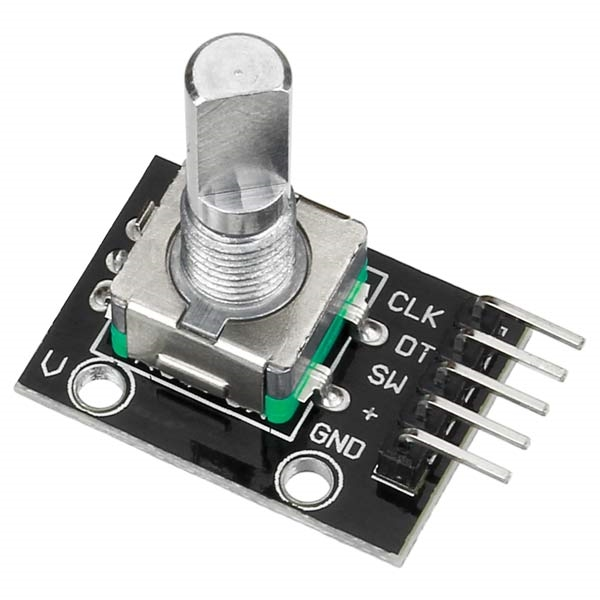
\includegraphics[scale=0.33]{enc_00}
	\captionsetup{justification=centering, margin=1.5cm}
	\centering
	\caption{Incremental Rotary Encoder}
	\centering
\end{figure}

\subsection{Incremental Rotary Encoders}\label{encoders_how_they_work}

As previously mentioned, an incremental encoder measure changes in position, but it does not keep track of absolute position.\\
It is also known as Quadrature Encoder since its A and B output signals are two square waves in quadrature.

%\begin{figure}[!ht]
%	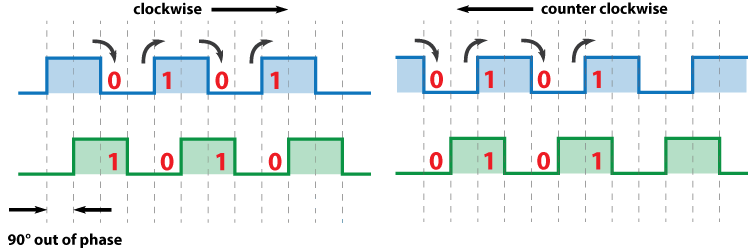
\includegraphics[scale=0.5]{enc_02}
%	\captionsetup{justification=centering, margin=1.5cm}
%	\centering
%	\caption{Incremental Encoder, output signals A and B.}
%	\centering
%\end{figure}

\begin{figure}[!ht]
	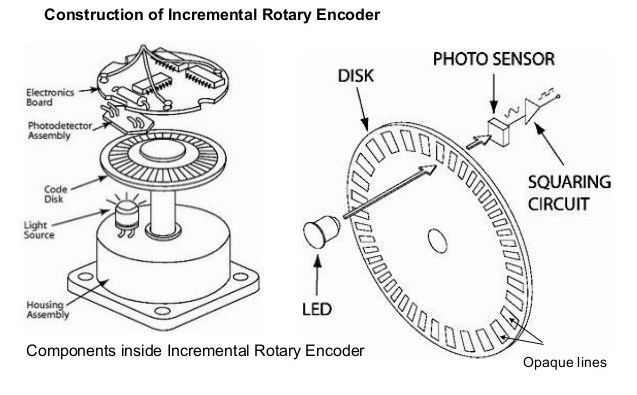
\includegraphics[scale=0.6]{enc_structure_00}
	\captionsetup{justification=centering, margin=1.5cm}
	\centering
	\caption{Encoder internal structure.}
	\centering
\end{figure}

%We can imagine the encoder as composed of a disk with evenly spaced contact zones, connected to a common pin and two other separate contact pins A and B. The disk rotates together with the shaft; while it rotates the pins A and B will start making contact with the common pin and the two square wave output signals will be generated accordingly.\\
The encoder is composed of a disk with evenly spaced opaque lines. On one side of the disk there is a light source, while on the other side there are two photodetectors, which are generating the signals A and B. The disk rotates together with the shaft, while it rotates the opaque lines will pass between the light source and the photodetectors generating the square waves.



\begin{figure}[htb]
 \centering
	\begin{subfigure}{0.2\textwidth}
		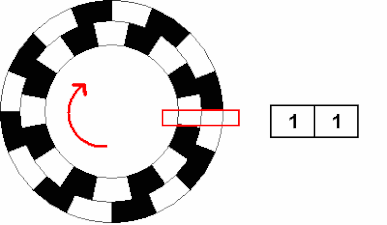
\includegraphics[width=\linewidth]{enc_principle_01}
	\end{subfigure}\hfil
	\begin{subfigure}{0.2\textwidth}
		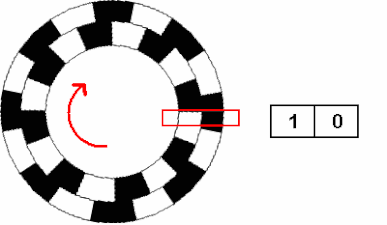
\includegraphics[width=\linewidth]{enc_principle_02}
	\end{subfigure}\hfil
	\begin{subfigure}{0.2\textwidth}
		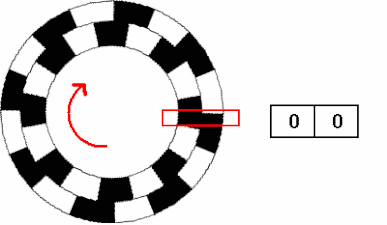
\includegraphics[width=\linewidth]{enc_principle_03}
	\end{subfigure}\hfil
	\begin{subfigure}{0.2\textwidth}
		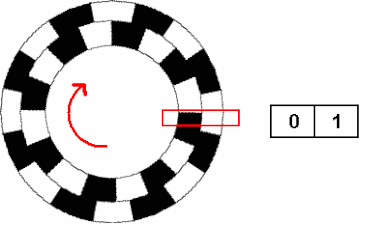
\includegraphics[width=\linewidth]{enc_principle_04}
	\end{subfigure}
	\captionsetup{justification=centering, margin=1.5cm}
	\caption{Generation of the square wave otuput pulses for clockwise rotations.}
\end{figure}

\begin{figure}[htb]
 \centering
	\begin{subfigure}{0.2\textwidth}
		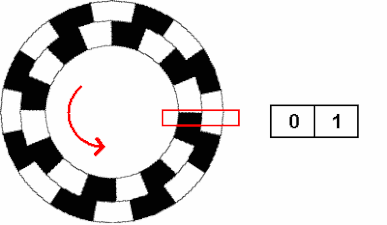
\includegraphics[width=\linewidth]{enc_principle_05}
	\end{subfigure}\hfil
	\begin{subfigure}{0.2\textwidth}
		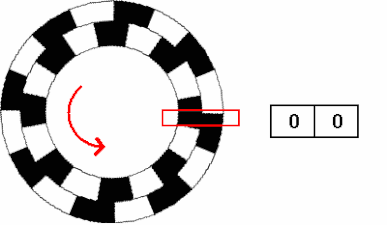
\includegraphics[width=\linewidth]{enc_principle_06}
	\end{subfigure}\hfil
	\begin{subfigure}{0.2\textwidth}
		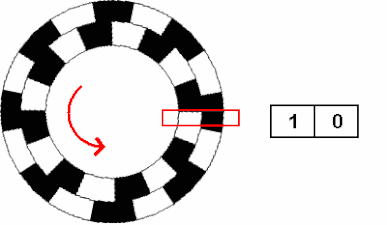
\includegraphics[width=\linewidth]{enc_principle_07}
	\end{subfigure}\hfil
	\begin{subfigure}{0.2\textwidth}
		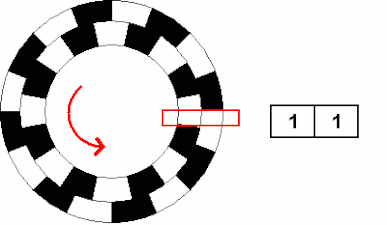
\includegraphics[width=\linewidth]{enc_principle_08}
	\end{subfigure}
	\captionsetup{justification=centering, margin=1.5cm}
	\caption{Generation of the square wave otuput pulses for anti-clockwise rotations.}
\end{figure}

The frequency of the pulses in the A and B output is directly proportional to the shaft rotational velocity; higher frequencies indicate rapid movement, whereas lower frequencies indicate slower speeds. Static, unchanging signals A and B indicate the encoder is motionless.


%https://www.youtube.com/watch?v=v4BbSzJ-hz4
%https://en.wikipedia.org/wiki/Incremental_encoder

\section{Inertial Measurement Unit}

There are mainly two categories of IMUs: stable platform systems and strapdown systems. The main difference between the two is the frame of reference in which the sensor operates.
\begin{itemize}
	\item In stable platform systems the inertial sensors are mounted on a platform isolated from any external motion; therefore the sensor always keep its alignment with the global frame.
	\item Strapdown systems instead are mounted rigidly on the platform, therefore the sensor is always aligned with the body frame (i.e. the navigation system's frame of reference).
\end{itemize}
In the following, we will consider strapdown systems as such is the one used in the robot we are considering.\\
Since the output is relative to the body frame, to keep track of the orientation gyroscope measurements must be integrated, and to keep track of the position accelerometer measurements are projected onto the global axis (using the orientation determined through the gyroscope) and then they are integrated\label{imu_integration}.\supercite{intro_inertial_navigation}
\begin{figure}[!ht]
	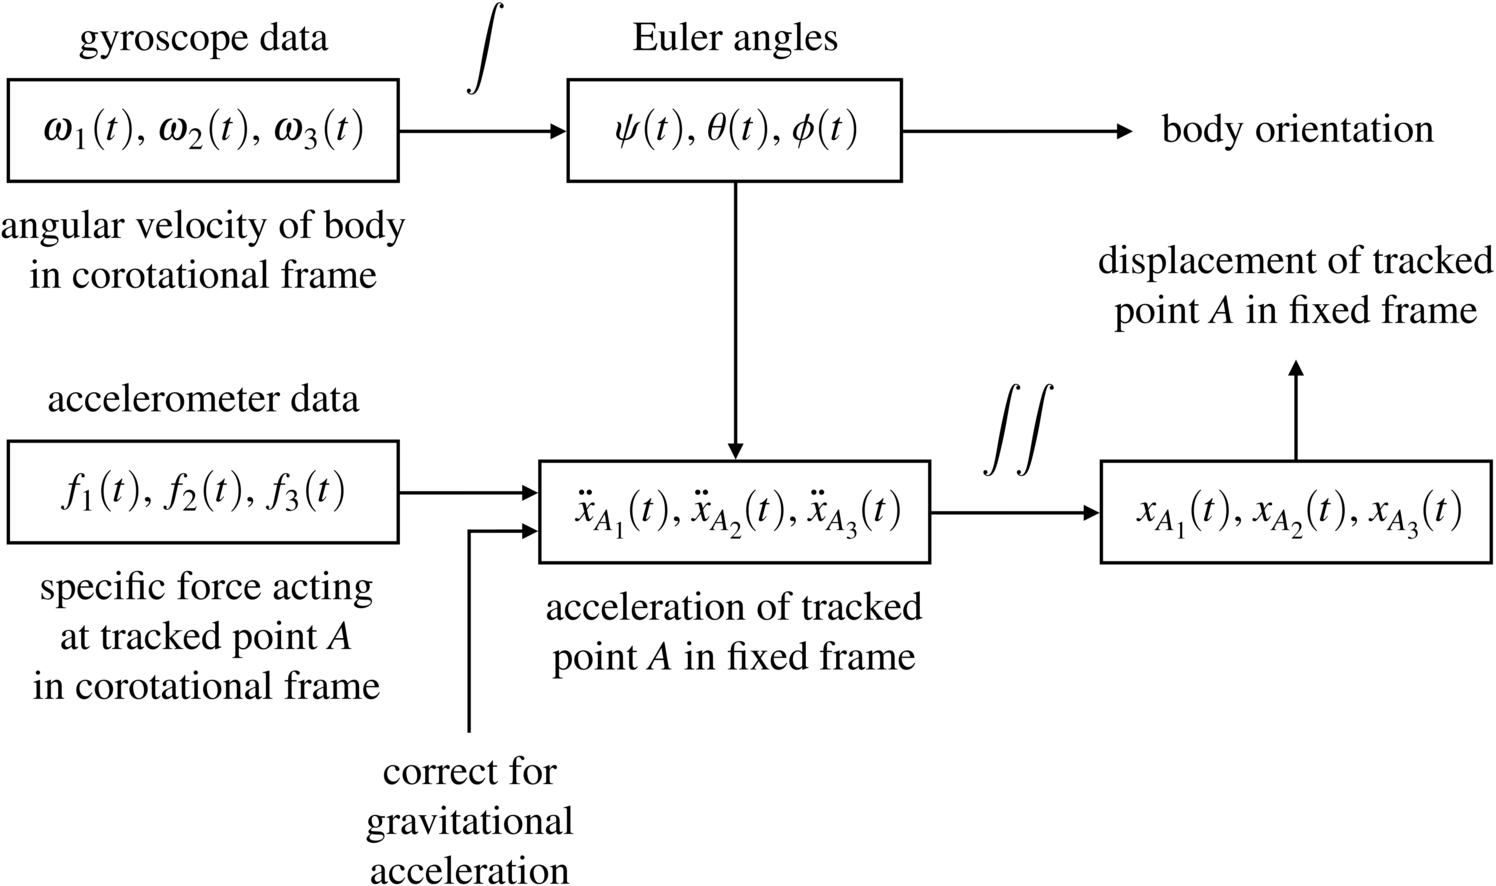
\includegraphics{imu_integration_40}
	\captionsetup{justification=centering, margin=1.5cm}
	\centering
	\caption{Strapdown Inertial Navigation Algorithm.}
	\centering
\end{figure}



\subsection{Gyroscope}

Gyroscopes are devices that measure rotational motion. While conventional gyroscopes measure orientation, most modern gyroscopes are rate-gyros measuring angular velocity.\\
\subsubsection{Mechanical Gyroscope}

A mechanical gyroscope consists of a spinning wheel mounted on two gimbals which allow it to rotate in all three axis. As an effect of the conservation of angular momentum, the spinning wheel will resist orientation changes. Hence when a gyroscope is subject to rotation, the wheel will keep rotating around the same rotational axis, while the angles between adjacent gimbals will change. Therefore to measure the orientation we have to measure angles between adjacent gimbals.\\
\begin{figure}[!ht]
	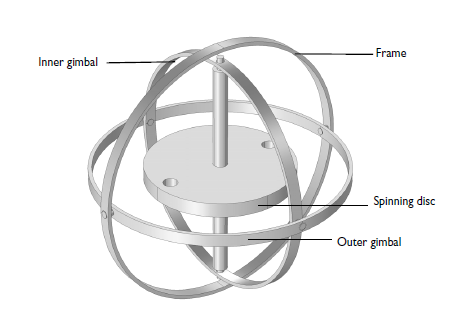
\includegraphics[scale=0.89]{mechanical_gyroscope}
	\captionsetup{justification=centering, margin=1.5cm}
	\centering
	\caption{Mechanical Gyroscope.}
	\centering
\end{figure}

\subsubsection{MEMS Gyroscope}

Unlike mechanical gyroscopes, MEMS gyros use the Coriolis effect to measure angular velocities. When a mass \textit{m} is moving with velocity \textit{v}, within a reference frame rotating at angular velocity \textit{$\omega$}, it experiences an apparent force:
\begin{gather*}
	F_c = -2m(\omega*v)
\end{gather*}

In MEMS gyros, vibrating elements are used to measure the Coriolis effect. In a simple configuration, there is a single mass allowed to vibrate along a drive axis; when the gyro is rotated, a second vibration occurs along the perpendicular sense axis due to the Coriolis effect. The angular velocity can be calculated from this second movement.

%\begin{figure}[!ht]
%	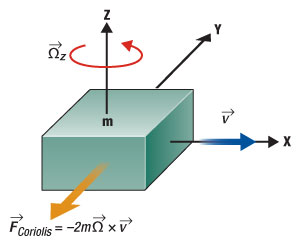
\includegraphics[scale=0.8]{mems_gyro_01}
%	\captionsetup{justification=centering, margin=1.5cm}
%	\centering
%	\caption{The Coriolis Force.}
%	\centering
%\end{figure}

\begin{figure}[htb]
 \centering
	\begin{subfigure}{0.45\textwidth}
		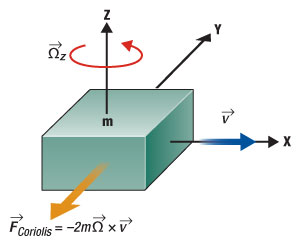
\includegraphics[width=\linewidth]{mems_gyro_01}
		\caption{The Coriolis Force.}
	\end{subfigure}\hfil
	\begin{subfigure}{0.45\textwidth}
		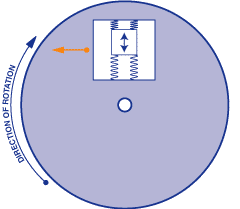
\includegraphics[width=\linewidth]{mems_gyro_02}
		\caption{MEMS Gyroscope.}
	\end{subfigure}
\end{figure}

Compared to conventional mechanical gyros, MEMS gyros are smaller and becoming cheaper, but they are not always as accurate as the former ones.

%\begin{figure}[!ht]
%	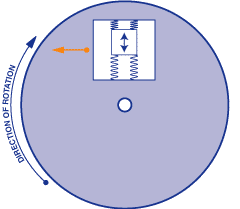
\includegraphics[scale=0.7]{mems_gyro_02}
%	\captionsetup{justification=centering, margin=1.5cm}
%	\centering
%	\caption{MEMS gyroscope.}
%	\centering
%\end{figure}

%references
%https://electroiq.com/2010/11/introduction-to-mems-gyroscopes/
%https://learn.sparkfun.com/tutorials/gyroscope [only image]
%supercite{intro_inertial_navigation}


\subsection{Accelerometer}

Accelerometers are devices that measure accelerations (i.e. the rate of change of the velocity of an object).

\subsubsection{Mechanical Accelerometer}

A mechanical accelerometer consists of a mass suspended by springs. When an acceleration occurs, as an effect of the principle of inertia, the mass will resist to any change in its velocity and the spring stretches with a force proportional to the acceleration (according to Newton's second law \textit{F = ma}). Therefore the distance the spring stretches can be used to measure the acceleration.

\begin{figure}[!ht]
	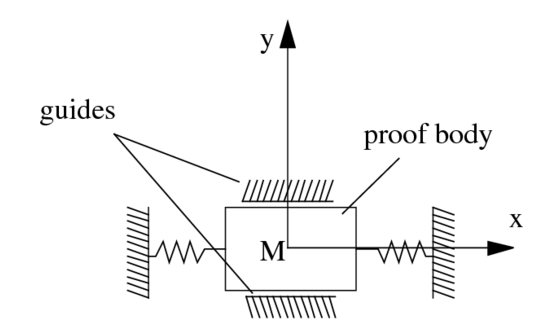
\includegraphics[scale=0.7]{mechanical_accelerometer_02}
	\captionsetup{justification=centering, margin=1.5cm}
	\centering
	\caption{Mechanical Accelerometer.}
	\centering
\end{figure}

\subsubsection{MEMS Accelerometer}

MEMS accelerometers usually contain capacitive plates internally. Some of these are fixed, while others are attached to springs and therefore able to move when subject to acceleration forces. As these plates move in relation to each other, the capacitance between them changes. Therefore measuring the capacitance we can determine the acceleration acting on the sensor.

%\begin{figure}[!ht]
%	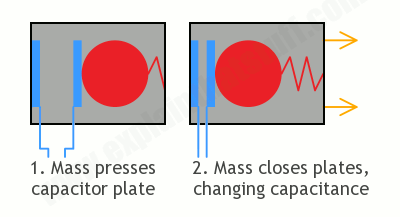
\includegraphics[scale=0.7]{capacitive_accelerometer}
%	\captionsetup{justification=centering, margin=1.5cm}
%	\centering
%	\caption{Capacitive Accelerometer.}
%	\centering
%\end{figure}

%\begin{figure}[!ht]
%	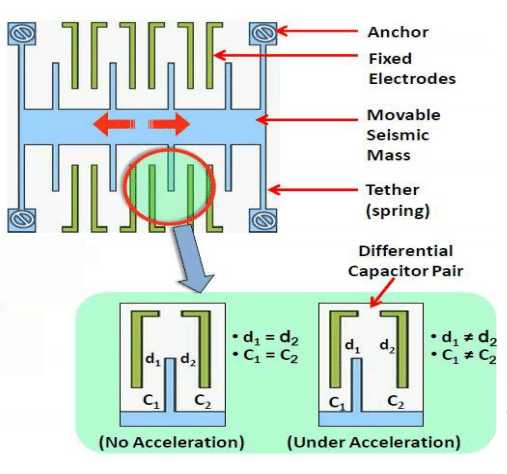
\includegraphics[scale=0.7]{mems_accelerometer_00}
%	\captionsetup{justification=centering, margin=1.5cm}
%	\centering
%	\caption{Capacitive Accelerometer.}
%	\centering
%\end{figure}

\begin{figure}[htb]
 \centering
	\begin{subfigure}{0.48\textwidth}
		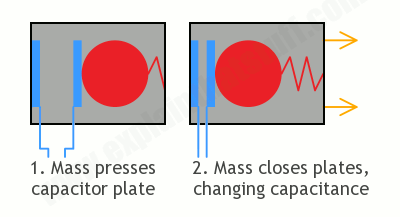
\includegraphics[width=\linewidth]{capacitive_accelerometer}
		\caption{Capacitive Accelerometer.}
	\end{subfigure}\hfil
	\begin{subfigure}{0.48\textwidth}
		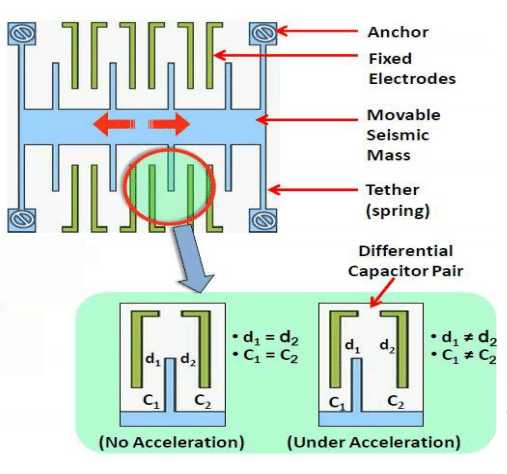
\includegraphics[width=\linewidth]{mems_accelerometer_00}
		\caption{MEMS Accelerometer.}
	\end{subfigure}
\end{figure}

%references
%https://www.explainthatstuff.com/accelerometers.html [mechanical]
%http://mafija.fmf.uni-lj.si/seminar/files/2007_2008/MEMS_accelerometers-koncna.pdf[mems]
%https://www.youtube.com/watch?v=KZVgKu6v808[mems]

\subsection{MEMS Sensors Error Characteristics}\label{mems_errors}

MEMS sensors are subject to many possible different errors; in the following we will explain only the ones we took in consideration calibrating our sensors (we will describe the calibration process we used in Section \ref{imu_calib}).
\begin{itemize}
	\item \textbf{Constant Biases}. The bias of a MEMS sensor is the average value it outputs in a motionless state.
	\item \textbf{Scale Factor Erros}. The scale factor should convert the digital quantity measured by each sensor into real physical quantities (e.g, accelerations and gyro rates). Unfortunately, MEMS based IMUs are affected by non-accurate scaling; therefore the scale factor tends to be slightly different from the one expected, and the 3-axes of the same sensor may have different scale factors.
	\item \textbf{Thermo-Mechanical White Noise}. The output of MEMS sensors is also affected by a zero-mean thermo-mechanical noise.
\end{itemize}

\chapter{Robot Details}

In this chapter we will examine the robot's architecture and details.

\section{Hardware}

The robot in discussion includes two encoders and an IMU in order to have motion's observation and be able, in the firmware's logic, to compute the odometry of the robot.\\
We have used :
\begin{itemize}
	\item a Mega2560 board\supercite{mega2560_datasheet},
	\item two rotary encoders KY-040\supercite{enc_datasheet},
	\item an IMU 10DOF MPU 9250\supercite{imu_prod_spec}.
\end{itemize}


\begin{figure}[htb]
 \centering
	\begin{subfigure}{0.3\textwidth}
		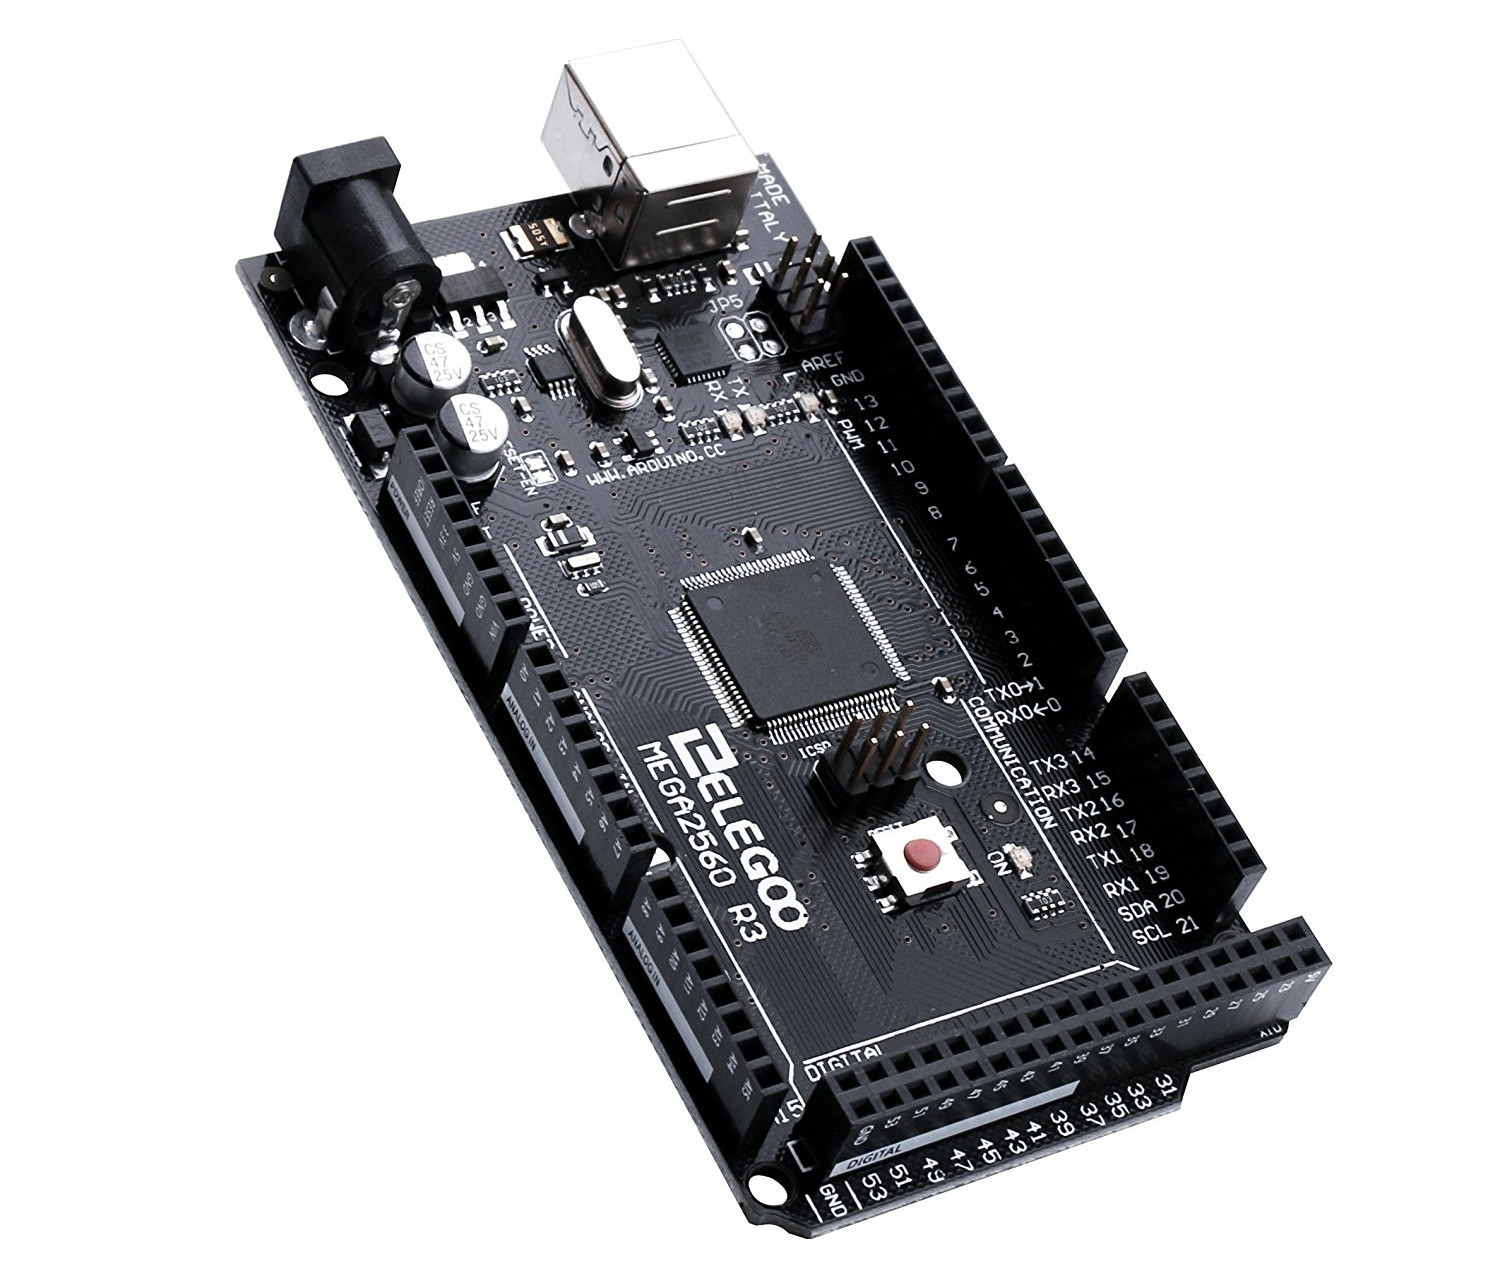
\includegraphics[width=\linewidth]{mega2560_00}
		\captionsetup{justification=centering}
		\caption{A Mega2560 board,}
	\end{subfigure}\hfil
	\begin{subfigure}{0.3\textwidth}
		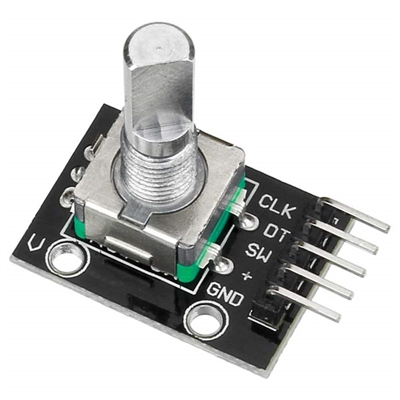
\includegraphics[width=\linewidth]{encs_ky_040}
		\captionsetup{justification=centering}
		\caption{two rotary encoders KY-040,}
	\end{subfigure}\hfil
	\begin{subfigure}{0.3\textwidth}
		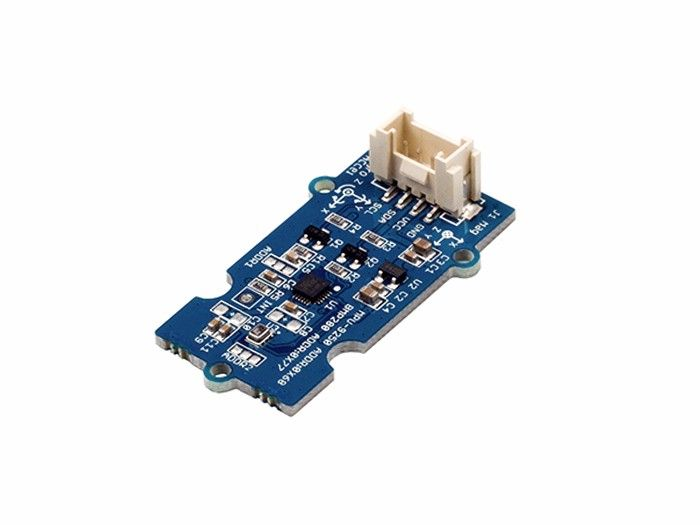
\includegraphics[width=\linewidth]{imu_mpu9250}
		\captionsetup{justification=centering}
		\caption{an IMU 10DOF MPU 9250.}
	\end{subfigure}
	\captionsetup{justification=centering, margin=1.5cm}
	\centering
	\caption{Hardware used for the robot.}
\end{figure}
The encoders are connected to the wheels in order to measure the wheels' rotations, while the IMU is mounted in correspondence of the center of the robot (where as center of the robot we take the mid-point of the wheel axle) at a higher position in order to reduce the electromagnetic-noise given by the CPU computations.\\
\begin{figure}[htb]
 \centering
	\begin{subfigure}{0.43\textwidth}
		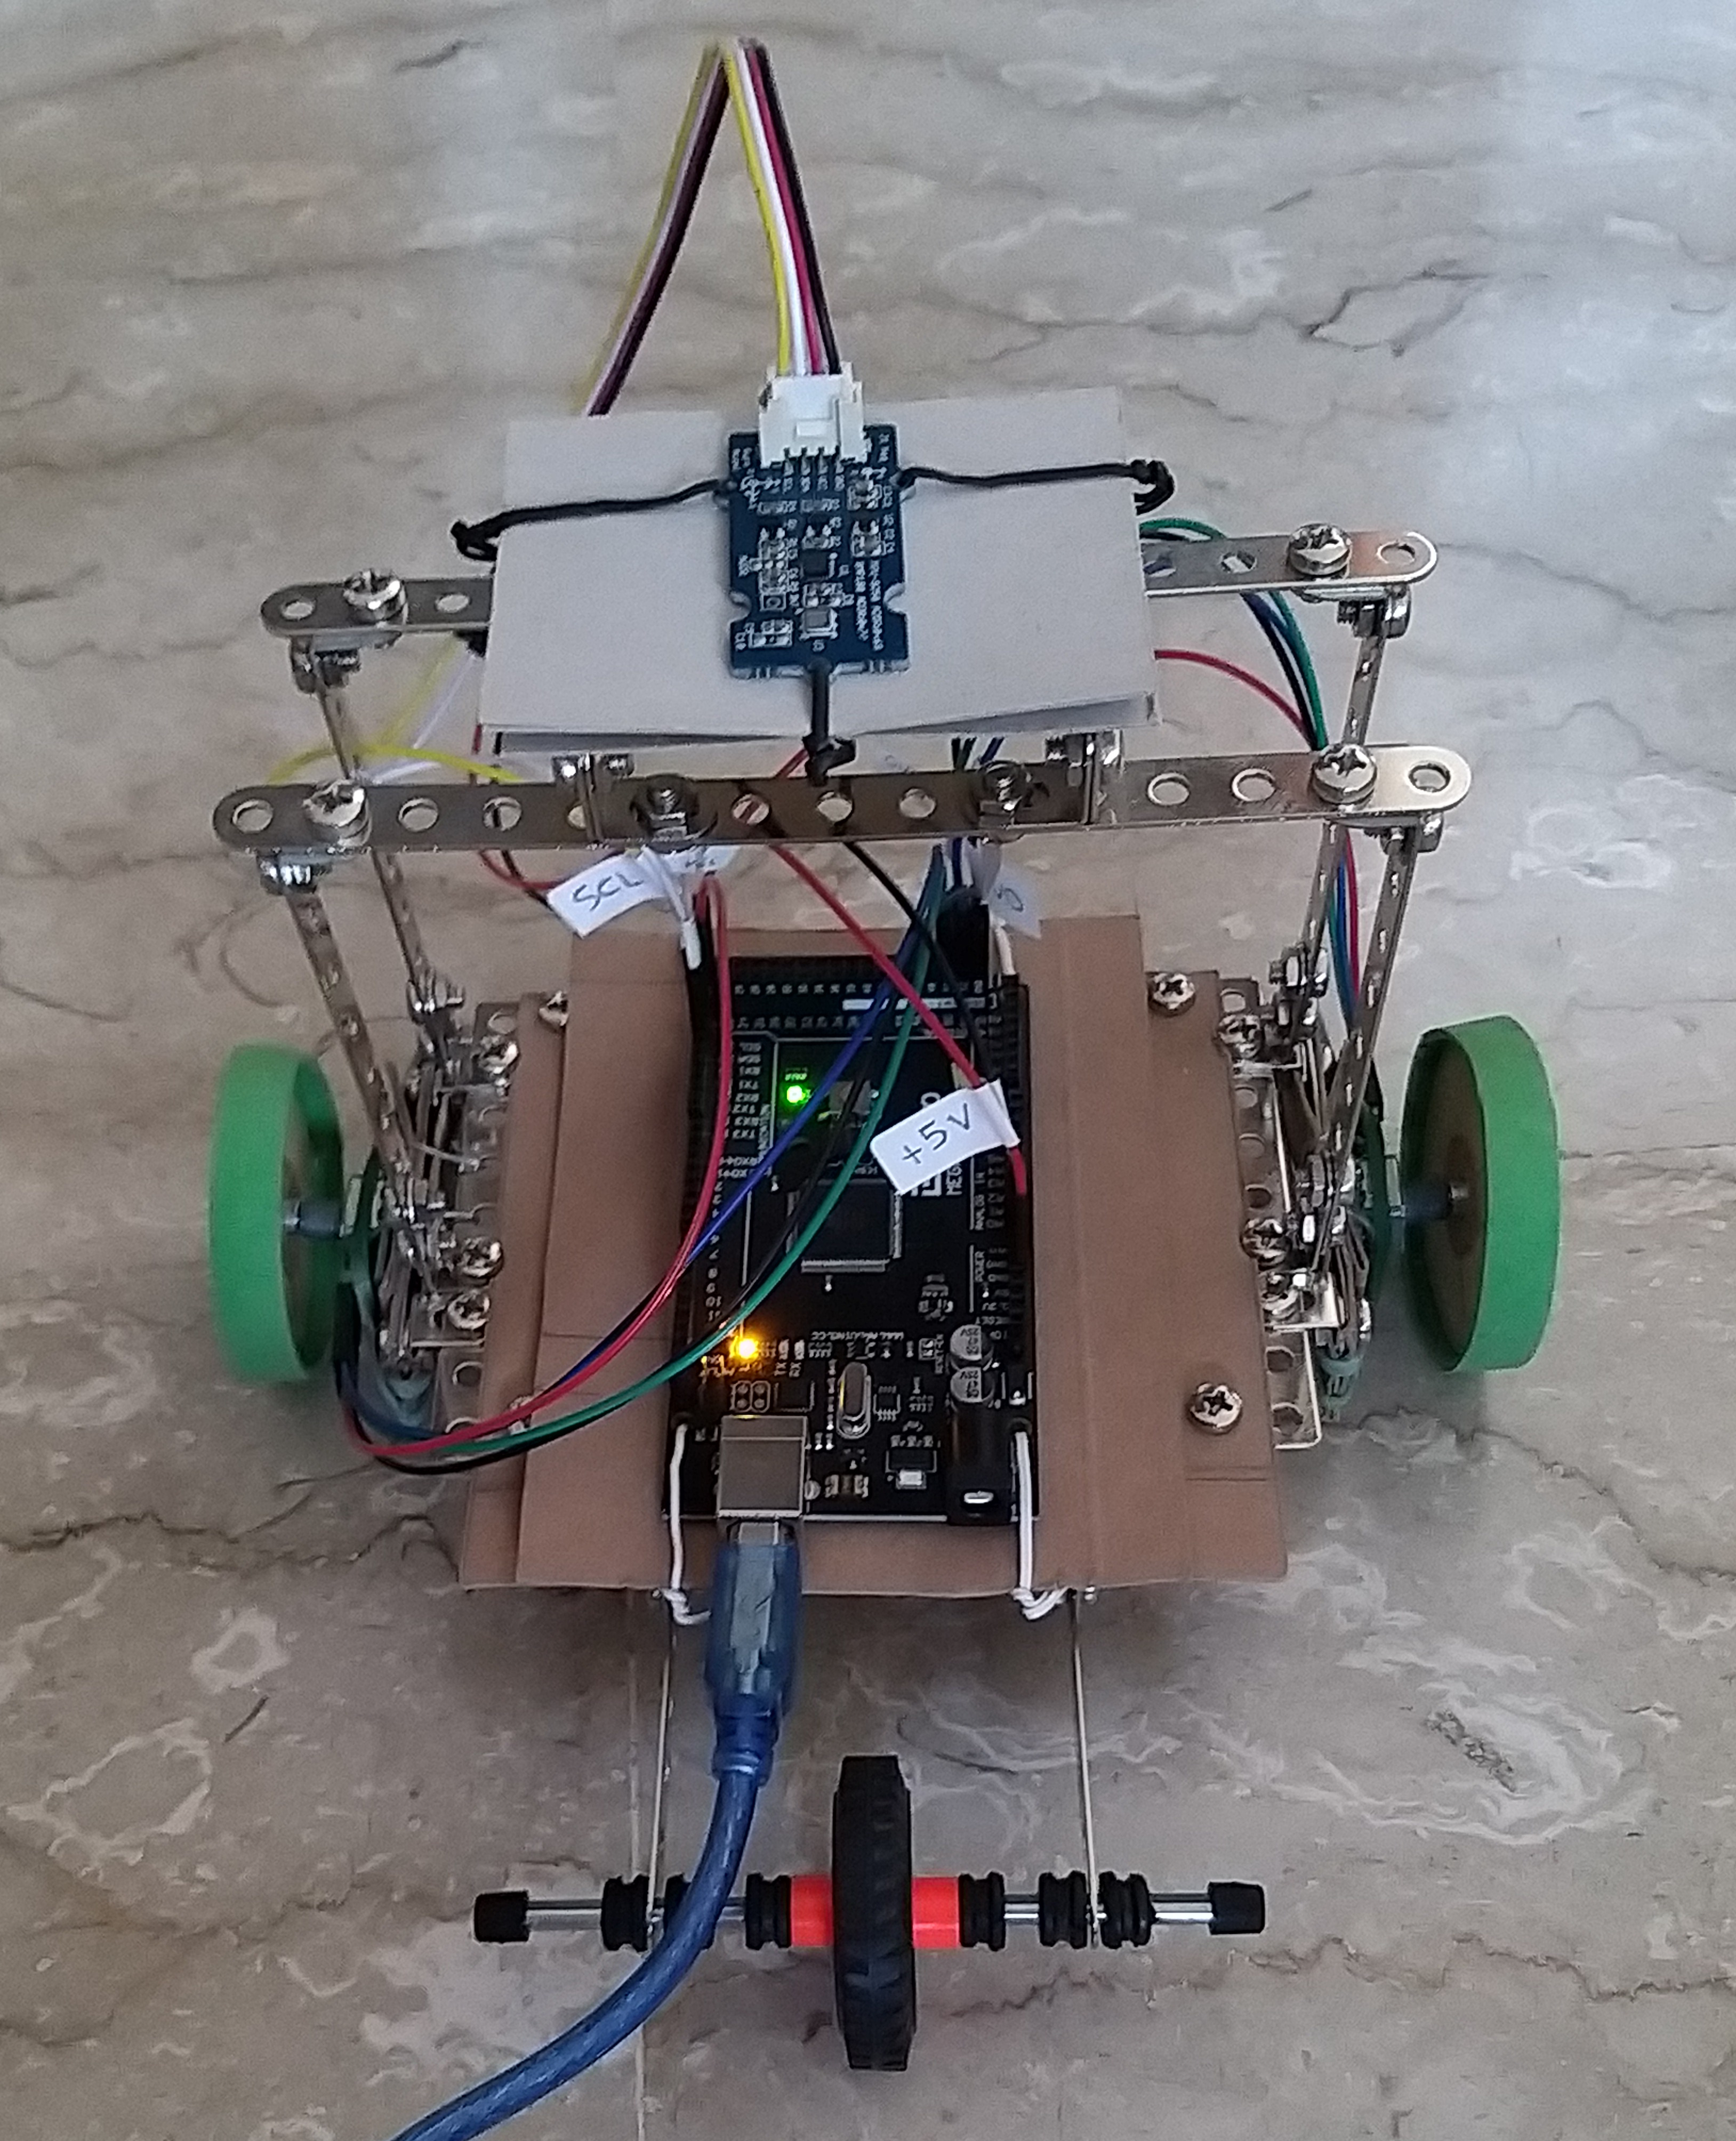
\includegraphics[width=\linewidth]{robot_image_01_20190701_085754_001}
	\end{subfigure}\hfil
	\begin{subfigure}{0.47\textwidth}
		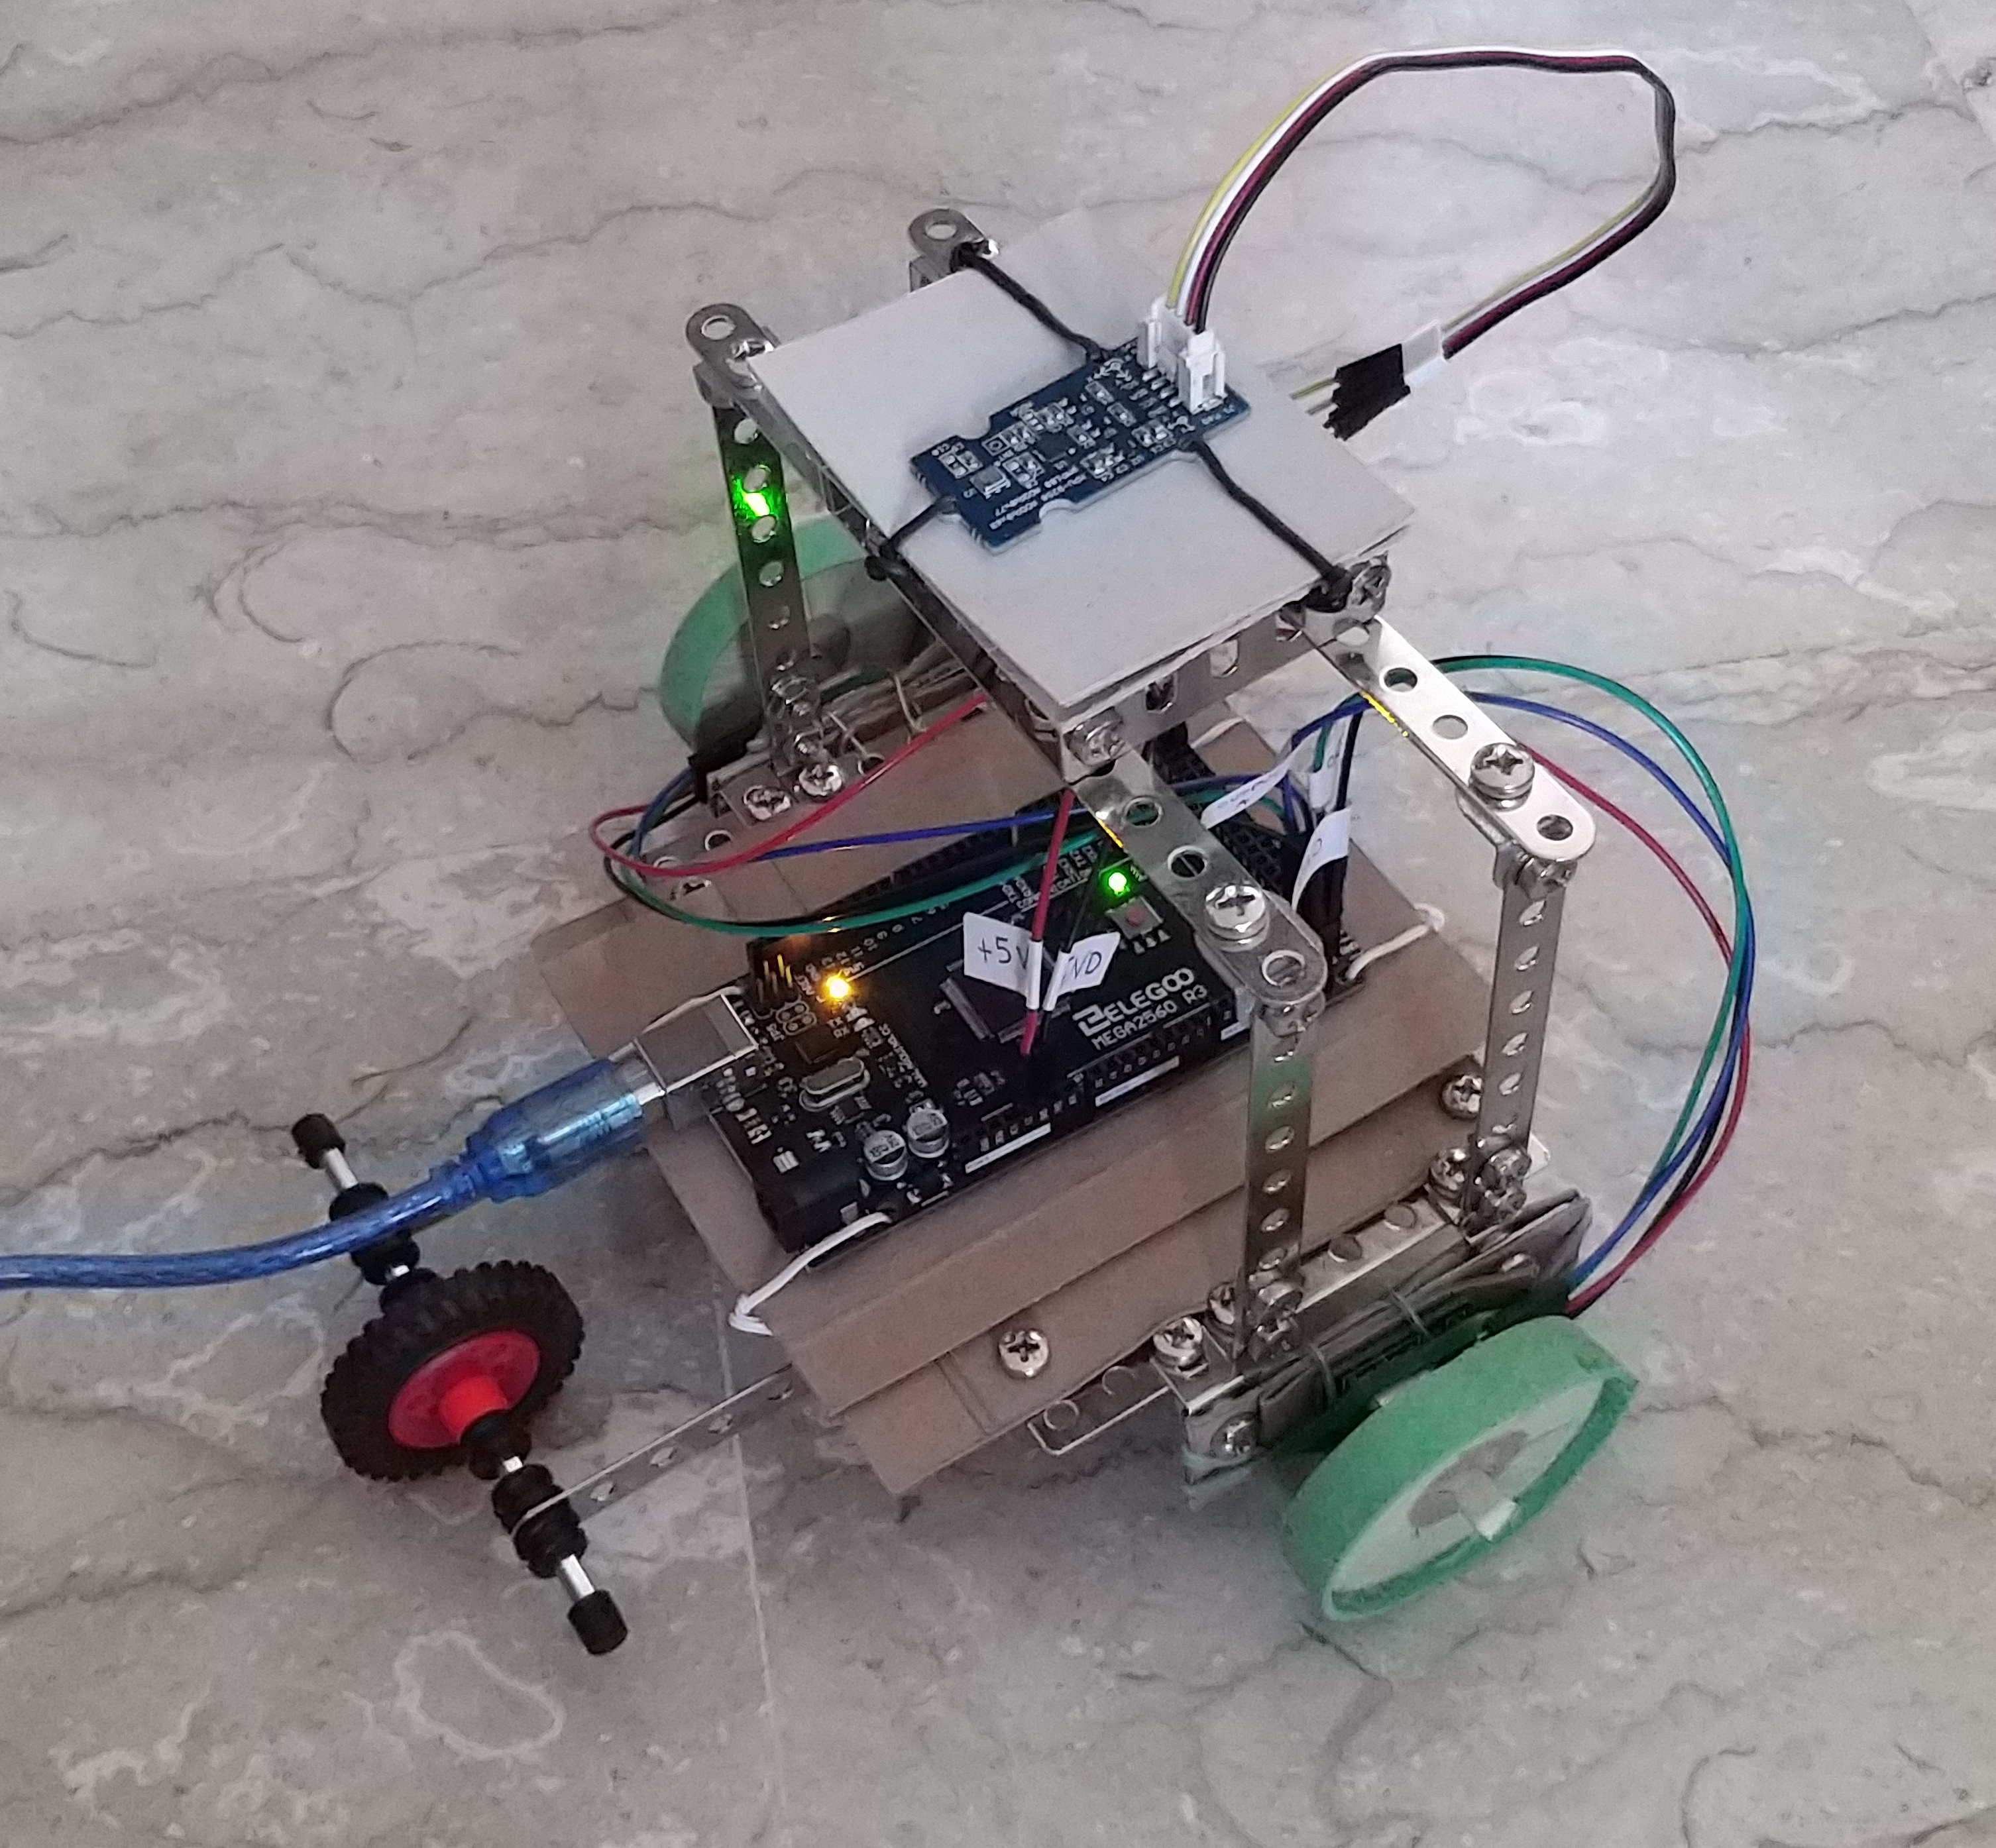
\includegraphics[width=\linewidth]{robot_image_06_20190701_085834}
	\end{subfigure}
	\captionsetup{justification=centering, margin=1.5cm}
	\centering
	\caption{Robot used for the tests.}
\end{figure}

\section{Communication Protocols}

In the development of the firmware we have used two communication protocols:
\begin{itemize}
	\item the I2C protocol to communicate with the IMU,
	\item the UART communication to interface with the host.
\end{itemize}
\subsection{I2C Protocol}

The I2C\footnote{I2C stands for Inter-Integrated Circuit} protocol is a synchronous serial computer bus. It enables multi-slave and multi-master modes, but we have used it in a simple configuration using the MEGA2560 board as master and the IMU as slave.\\

Each device on the bus has a preset ID so that the master can choose the slave to communicate with.\\
This bus uses two wires:
\begin{itemize}
	\item Serial Clock (SCL) for the clock signal (generated by the master) which synchronizes the communication between master and slave,
	\item Serial Data (SDA) carrying the data.
\end{itemize}

\begin{figure}[!ht]
	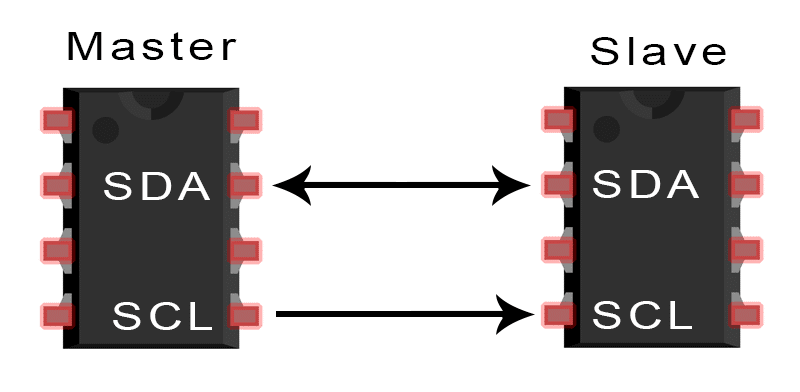
\includegraphics[scale=0.6]{i2c_master_slave}
	\captionsetup{justification=centering, margin=1.5cm}
	\centering
	\caption{I2C wires.}
	\centering
\end{figure}


The data signal is transferred in sequences of 8 bits, each of them synchronized with the clock signal.
\begin{itemize}
	\item The communication starts with the master sending a special START condition over the bus,
	\item then the master sends an 8-bit sequence indicating the address of the slave device to which the communication is addressed,
	\item at this point the master waits for the slave to send back an Acknowledgement (ACK).
	\item After this first Acknowledgement by the slave device, in most cases there is a second addressing sequence indicating the address of the internal register where to read or write.
	\item Finally the data is sent through the bus,
	\item and the communication ends with a STOP condition generated by the master.
\end{itemize}
\begin{figure}[!ht]
	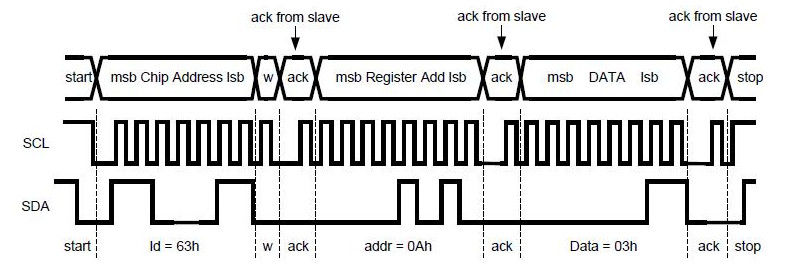
\includegraphics[scale=0.5]{i2c_protocol_01}
	\captionsetup{justification=centering, margin=1.5cm}
	\centering
	\caption{I2C general protocol.}
	\centering
\end{figure}

Let us now dig further in the protocol distinguishing the cases of reading and writing a register. To distinguish between a read and a write operation, in the first addressing cycle only the first 7 bits are actually used to identify the slave device, while the least significant bit is used to discriminate read and write operations [0 for a write operation, 1 for a read].
\begin{figure}[!ht]
	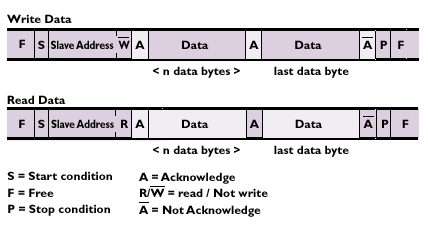
\includegraphics[scale=0.6]{i2c_protocol_02}
	\captionsetup{justification=centering, margin=1.5cm}
	\centering
	\caption{I2C protocol: distinguishing read and write operations.}
	\centering
\end{figure}

\paragraph{Write Operations}
A write operation is composed by a single write transaction, where the master sends two data bytes to the slave, the first one is the address of the internal register the master wants to write to, while the second one is the value the master wants to write in it.
\begin{itemize}
	\item[1. ] The master starts the transmission transmitting the start condition.
	\item[2. ] Then the master transmits the 7-bits device address, followed by the write bit (0), and waits for the slave to send an ACK.
	\item[3. ] At this point the master puts the address of the internal device register on the bus, and waits for the slave's ACK;
	\item[4. ] and next the master sends the data to be written, and waits for the slave's ACK. Eventually the master could go on sending more data which will be written in the following registers, waiting for the slave's ACK for each 8-bit data.
	\item[5. ] Finally the master transmits the stop condition to end the communication.
\end{itemize}

\paragraph{Read Operations}
A read operation is composed of a write transaction followed by a read transaction. In the write transaction the master sends to the slave the address of the register he wants to read, while in the read transaction the slave sends the value of the requested register to the master.
\begin{itemize}
	\item[1. ] The master starts the write transaction transmitting the start condition.
	\item[2. ] Then the master transmits the 7-bits device address, followed by the write bit (0), and waits for the slave to send an ACK;
	\item[3. ] and next the master puts the address of the internal device register on the bus, and waits for the slave's ACK.
	\item[4. ] At this point the master starts the read transaction retransmitting a start condition (restart).
	\item[5. ] Then the master transmits the 7-bits device address, followed by the read bit (1), and waits for the slave to send an ACK;
	\item[6. ] and next the slave puts the data to be read on the bus. The master will send an ACK only if more data (from the following registers) is expected, when the master does not want the slave to send more data on the bus it sends a NACK (Not-Acknowledgement). Therefore the slave will stop sending data only upon receiving a NACK.
	\item[7. ] Finally the master transmits the stop condition to end the communication.
\end{itemize}
See Appendix \ref{i2c_implementation} for an implementation of the I2C protocol.\\


\subsection{UART Communication}

The UART\footnote{UART stands for Universal Asynchronous Receiver-Transmitter} is a computer hardware device for asynchronous serial communication. It is not a communication protocol as I2C but a physical circuit on the microcontroller, whose main purpose is to transmit and receive serial data.\\

In UART communication, two devices communicate directly with each other. The transmitting UART converts parallel data into serial data, and then transmits it in serial to the receving UART, that is in charge of reconstructing the parallel data. Only two wires are used to transmit data between devices, each of them going from the Transmit (Tx) pin of a device to the Receive (Rx) pin of the other.

\begin{figure}[htb]
 \centering
	\begin{subfigure}{0.35\textwidth}
		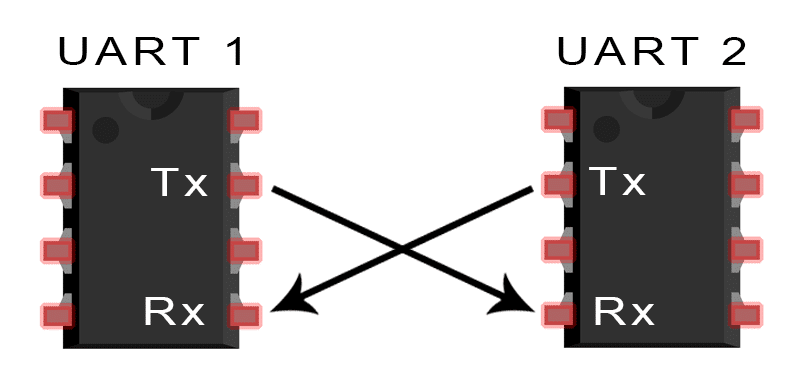
\includegraphics[width=\linewidth]{uart_tx_rx}
		\captionsetup{justification=centering}
		\caption{wires used for UART communication}
	\end{subfigure}\hfil
	\begin{subfigure}{0.6\textwidth}
		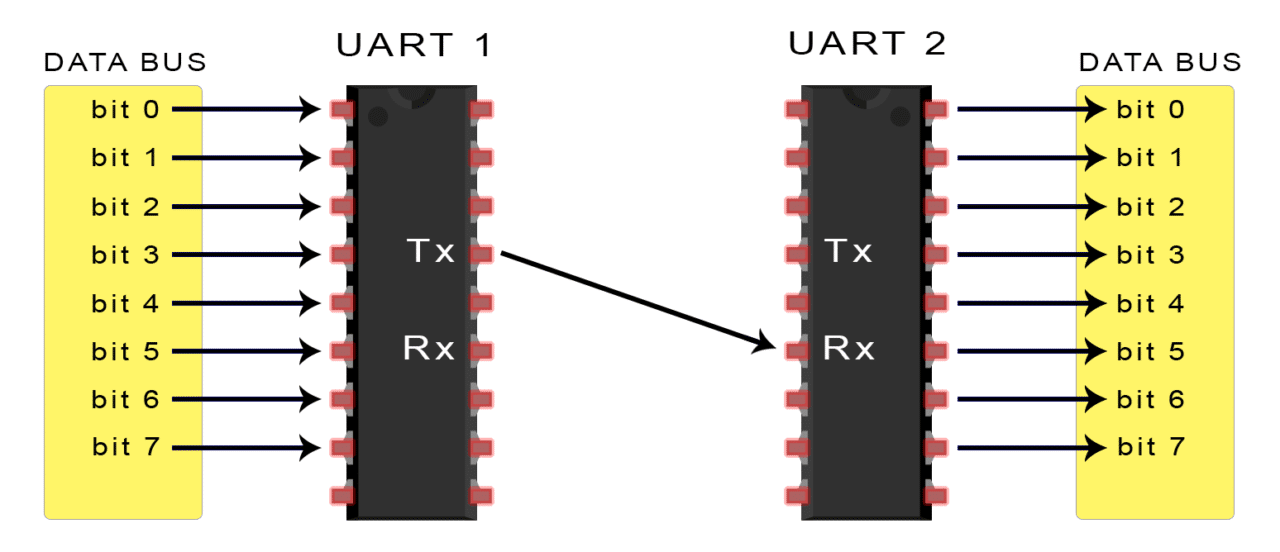
\includegraphics[width=\linewidth]{uart_parallel_to_serial}
		\captionsetup{justification=centering}
		\caption{parallel to serial data conversion for UART communication}
	\end{subfigure}
	\captionsetup{justification=centering, margin=1.5cm}
	\centering
	\caption{UART communication}
\end{figure}

\begin{itemize}
	\item[1. ] The transmitting CPU sends the data to be sent to the UART on a data bus, then the data is transferred from the data bus to the transmitting UART in parallel form.
	\item[2. ] The transmitting UART gets the parallel data from the bus and creates a data packet (adding a start bit, a parity bit and a stop bit).
					\begin{figure}[!ht]
						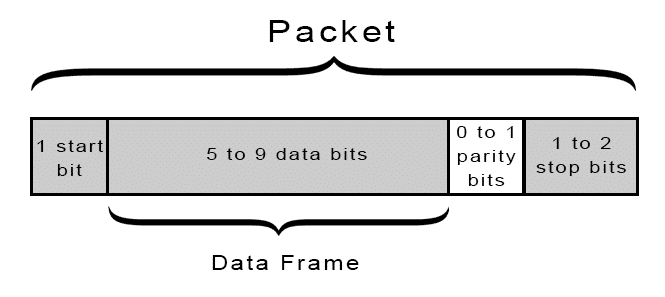
\includegraphics[scale=0.5]{uart_packet}
						\captionsetup{justification=centering, margin=1.5cm}
						\centering
						\caption{UART data packet.}
						\centering
					\end{figure}
	\item[3. ] The transmitting UART sends the data packet to the receiving UART serially, outputting it bit by bit from the Tx pin.
	\item[4. ] The receiving UART reads the packet bit by bit from the Rx pin,
	\item[5. ] and then converts the data received back into parallel form and removes the start bit, the parity bit and the stop bit.
	\item[6. ] Finally the receiving UART transfers the data to the receiving CPU on the data bus in parallel.
\end{itemize}
See Appendix \ref{uart_implementation} for an implementation of UART communication.\\

\section{Firmware}

All the firmware is designed to be interrupt driven. In addition to the interrupt driven implementation of the I2C protocol and the UART communication, the firmware's logic is based on timed interrupts. The sampling of the sensors and the update of the odometry is at a rate of 100 Hz, while the communication with the host is done at a rate of 1 Hz.

\subsection{Interpreting the Encoders Observations}

An encoder has two outputs A and B, which we have connected to two pins on the board.\\
When an encoder detects a rotation its outputs become two square waves (as described in \ref{encoders_how_they_work}), while when there is no rotation its outputs do not change their value. Therefore we have decided to use an interrupt solution, throwing an interrupt when one of the two pins changed its value.\\
We have connected the encoder corresponding to the left wheel to the pins 52-53 (PB1 and PB0 respectively\supercite{mega2560_datasheet}) while the one on the right wheel to the pins 50-51 (PB3 and PB2 respectively). Therefore we are using the first 4 pins of port B.
\begin{ccode}
	#define ENC_MASK 0xf //0b1111
	
	cli();

		//set the encoder pins as input
	DDRB &= ~ENC_MASK;
		//enable pull up resistors
	PORTB |= ENC_MASK;
		//set interrupt on change, looking up PCMSK0
	PCICR |= (1 << PCIE0);
		//tells which bits of the port triggers the interrupt
	PCMSK0 |= ENC_MASK;

	sei();
\end{ccode}
\captionof{lstlisting}{Installing the interrupt for handling the encoders.}

The ISR will then be responsible for the update of the state of the encoders. For each encoder we need to store:
\begin{itemize}
	\item a global counter, counting the total number of rotations the encoder has been subject to. Note that clockwise rotations increment the counter, while anticlockwise rotations decrement it.
	\item the previous value of the output pins, since in an incremental encoder the sense of the rotation is encoded in the transition between states.
\end{itemize}
\begin{ccode}
	typedef struct Encoder_t {
		uint8_t prev_value;	// previous value of the output pins
		int32_t counter;		// global counter of the encoder
	} Encoder_t;
\end{ccode}
\captionof{lstlisting}{Structure used to store all useful informations about encoders.}

Therefore the ISR recovers the actual and the previous values of the output pins and uses them to lookup in a transition table and update the encoder rotation counter.
\begin{ccode}
	#define NUM_ENCODERS 2
	
		//global variable storing the current state of the encoders
			//updated by the ISR
	static Encoder_t Encs[NUM_ENCODERS];
	
	static const int8_t _transition_table []= {
			0,	//0000
		 -1,	//0001
			1,	//0010
			0,	//0011
			1,	//0100
			0,	//0101
			0,	//0110
		 -1,	//0111
		 -1,	//1000
			0,	//1001
			0,	//1010
			1,	//1011
			0,	//1100
			1,	//1101
		 -1,	//1110
			0		//1111
	};

	// Interrupt Service Routine for PCINT0
	ISR(PCINT0_vect) {
		uint8_t port_value = PINB & ENC_MASK;
	
		uint8_t i;
		for(i=0; i<NUM_ENCODERS; i++){
				//we need the previous state, since in incremental encoders
					//we handle transitions from a state to the next
			Encs[i].prev_value <<=2;
			
				// port_value stores the new values of all encoders
					// with &0x03 we can handle an encoder at the time
					// and with >>= 2 t the end, we pass to the next encoder
			Encs[i].prev_value = Encs[i].prev_value | (port_value & 0x03);
			Encs[i].counter += _transition_table[Encs[i].prev_value & 0x0F];
		
			port_value >>= 2;
		}
	}
\end{ccode}
\captionof{lstlisting}{Installing the interrupt for handling the encoders.}


\subsection{Interpreting the IMU Observations}\label{imu_calib}

The IMU MPU9250 provides an I2C interface, through which we can access its control register and its 16-bit digital output registers\supercite{imu_prod_spec}.\\

\subsubsection{Initializing the IMU}

Reading the IMU datasheet\supercite{imu_prod_spec} and the register map\supercite{imu_regs} we were able to initialize the configuration registers according to our needs.\\

The gyroscope's full scale range was set to 250 DPS\footnote{DPS stands for Degrees Per Second}, hence it can observe only angular velocities in the range [-250 DPS, +250 DPS]. The accelerometer's full scale range instead was set to 2 G\footnote{1 G corresponds to the gravitational acceleration (i.e. $\sim 9.8 m/s^2$)} and therefore it can measure accelerations in the range [-2 G, +2 G].\\These are a quite small ranges but perfect for our needs since we do not expect the robot to exceed these bounds; moreover the use of small ranges gives us high sensitivity in these ranges.\\

The gyroscope's bandwidth, which is the highest frequency of angular velocity variation that can be detected by the sensor, was set to 41 Hz. The accelerometer's bandwidth instead was set to 44.8 Hz.\\According to the Nyquist Sampling Criterion, the rate at which the sensors are sampled must be at least twice the sensors' bandwidths. Therefore since we want to sample the IMU sensors at 100 Hz, we had to set the sensors' bandwidths below 50 Hz.
\begin{ccode}
	static void IMU_ConfigRegs(void) {
		//resets the internal registers and restores the default settings
		I2C_WriteRegister(ACCELGYRO_DEVICE, PWR_MGMT_1, 0x80);
		_delay_ms(500);
		
		//sets Gyroscope Full Scale range to 250dps (degrees/sec)
			//[low range, high sensitivity]
		I2C_WriteRegister(ACCELGYRO_DEVICE, GYRO_CONFIG, 0x00);
		_delay_ms(10);
	
		//sets Gyroscope bandwidth to 41Hz,
		I2C_WriteRegister(ACCELGYRO_DEVICE, CONFIG, 0x03);//41 Hz
		_delay_ms(10);
	
		//sets Accelerometer Full Scale to 2G
		I2C_WriteRegister(ACCELGYRO_DEVICE, ACCEL_CONFIG, 0x00);
		_delay_ms(10);
		
		//sets Accelerometer bandwidth to 44.8 Hz
		I2C_WriteRegister(ACCELGYRO_DEVICE, ACCEL_CONFIG2, 0x03);//44.8 Hz
		_delay_ms(10);

		//sets PowerManagement Registers
			//auto selects the best available clock source
			//and disables the sleep mode
		I2C_WriteRegister(ACCELGYRO_DEVICE, PWR_MGMT_1, 0x01);
		_delay_ms(10);
		
		//sets all sensors to on
		I2C_WriteRegister(ACCELGYRO_DEVICE, PWR_MGMT_2, 0x00);
		_delay_ms(10);
	
		//i2c_master interface pins(SCL, SDA)
			//will go into "bypass mode"
			//when the i2c master interface is disabled
		I2C_WriteRegister(ACCELGYRO_DEVICE, INT_PIN_CFG, 0x02);
		_delay_ms(10);
	}
\end{ccode}
\captionof{lstlisting}{IMU initialization of configuration registers.}

\subsubsection{Reading IMU registers}

As mentioned in the previous paragraph, we want to sample the IMU sensors at a rate of 100 Hz. Therefore we defined a timed interrupt with a frequency of 100 Hz and we gave to the corresponding interrupt service routine the task of reading the IMU data registers.
\begin{ccode}
	#define IMU_UPDATE_RATE 100 //Hz

	//from a frequency in Hz, we get a period in millisecs
 uint16_t period_ms = 1000 / IMU_UPDATE_RATE;
 
 //configure timer3, prescaler : 256, CTC (Clear Timer on Compare match)
 TCCR3A = 0;
 TCCR3B = (1 << WGM12) | (1 << CS12); 
 
 /*
	 * cpu frequency 16MHz = 16.000.000 Hz
	 * prescaler 256
	 *	-->> TCNT3 is increased at a frequency of 16.000.000/256 Hz = 62500 Hz
	 *	so 1 ms will correspond do 62.5 counts
	 */
 OCR3A = (uint16_t)(62.5 * period_ms);

	// timer-interrupt enabling must be executed atomically (no other interrupts)
		// and ATOMIC_FORCEON ensures Global Interrupt Status flag bit in SREG set afetrwards
 ATOMIC_BLOCK(ATOMIC_FORCEON) {
 	TIMSK3 |= (1 << OCIE3A);
 }
\end{ccode}
\captionof{lstlisting}{Installing the timed-interrupt to periodically read the IMU data registers.}

\begin{ccode}
	ISR(TIMER3_COMPA_vect) {
		//reads the accelerometer and the gyroscope data registers
		IMU_AccelGyroRaw();

		//increases the time stamp
		IMU.imu_time_seq++;
	}
\end{ccode}
\captionof{lstlisting}{ISR in charge of reading the IMU data registers.}

The output data from the accelerometer and the gyroscope are 16-bit values for each axis, divided in two 8-bit registers. Since the 6 registers for the accelerometer and the six ones for the gyroscope are consecutive, we can read them in a single I2C communication cycle and then reconstruct the 16-bit digital values.

\subsubsection{Calibrating the IMU sensors}

As described in paragraph \ref{mems_errors}, MEMS sensors are subject to errors, some of which can be compensated through a prior calibration process\supercite{imu_calib_01}\supercite{imu_calib_02}.\\

To compensate constant bias errors for the accelerometer and the gyroscope, we calculate the calibration biases by taking a long term average of the sensors' outputs while the IMU is motionless.\\
To compensate the scale factor errors of the accelerometer, we use a very simple multi-position scheme. By keeping the IMU with its z-axis upwards (aligned with the vertical gravity field) we expect to measure an acceleration of 1 G along the z-axis; therefore we can use the digital output of the sensor as the scale factor of the z-axis. By aligning the other axes with the gravity field, we calculate the scale factors for all the other axes of the accelerometer.\\
We have calculated the scale factors of the gyroscope starting from the full scale range. Since we expect the full scale range to correspond to the maximum value of the digital output, we have calculated the scale factor by dividing the maximum digital value by the maximum physically meaningful value than can be measured: $scale\_factor = 2^{15} / 250$. We did not compensate the scale factor errors of the gyroscope.\\

\begin{ccode}
	#define CALIBRATION_SAMPLES	128
	#define CALIBRATION_SAMPLES_LOG	7

	#define IMU_POS_Z_UP 0 // z-axis upwards
	#define IMU_POS_X_UP 1 // x-axis upwards
	#define IMU_POS_Y_UP 2 // y-axis upwards
	#define IMU_POS_Z_DOWN 3 // z-axis downwards
	#define IMU_POS_X_DOWN 4 // x-axis downwards
	#define IMU_POS_Y_DOWN 5 // y-axis downwards
	#define IMU_N_POS 6 //max number if positions
	
	int32_t gyro_x_sum[IMU_N_POS]={}, gyro_y_sum[IMU_N_POS]={}, gyro_z_sum[IMU_N_POS]={};
	int32_t accel_x_sum[IMU_N_POS]={}, accel_y_sum[IMU_N_POS]={}, accel_z_sum[IMU_N_POS]={};
	
	uint8_t p, i, orientation;
	
	for(p=0; p < IMU_N_POS; p++) {
		//waits for the robot is in a new orientation
			// ...
		
		//sets ths local variable to the current IMU orientation
		orientation = <imu_orientation>;
			
		//get samples
		for(i=0; i<CALIBRATION_SAMPLES; i++) {	
			gyro_x_sum[orientation] += <gyro_raw_x_observation>;
			gyro_y_sum[orientation] += <gyro_raw_y_observation>;
			gyro_z_sum[orientation] += <gyro_raw_z_observation>;
			
			accel_x_sum[orientation] += <accel_raw_x_observation>;
			accel_y_sum[orientation] += <accel_raw_y_observation>;
			accel_z_sum[orientation] += <accel_raw_z_observation>;
		}

		gyro_x_sum[orientation] >>= CALIBRATION_SAMPLES_LOG;
		gyro_y_sum[orientation] >>= CALIBRATION_SAMPLES_LOG;
		gyro_z_sum[orientation] >>= CALIBRATION_SAMPLES_LOG;

		accel_x_sum[orientation] >>= CALIBRATION_SAMPLES_LOG;
		accel_y_sum[orientation] >>= CALIBRATION_SAMPLES_LOG;
		accel_z_sum[orientation] >>= CALIBRATION_SAMPLES_LOG;
	}
	
	// GYROSCOPE
	int32_t gyro_total_x_sum=0, gyro_total_y_sum=0, gyro_total_z_sum=0;
	for(p=0; p<6; p++) {
		gyro_total_x_sum += gyro_x_sum[p];
		gyro_total_y_sum += gyro_y_sum[p];
		gyro_total_z_sum += gyro_z_sum[p];
	}
	
		//calculates the gyro's constant biases
	int32_t gyro_x_bias = (int16_t)(gyro_total_x_sum / 6);
	int32_t gyro_y_bias = (int16_t)(gyro_total_y_sum / 6);
	int32_t gyro_z_bias = (int16_t)(gyro_total_z_sum / 6);
	
		//calculates the gyro's scale factor (no calibration)
	float gyro_sensitivity = (float)((uint16_t)(1<<15) / 250.);

	float gyro_x_scale = gyro_sensitivity;
	float gyro_y_scale = gyro_sensitivity;
	float gyro_z_scale = gyro_sensitivity;
	
	//ACCELEROMETER	
	//asse X
		//to calculate the bias, we take in consideration the positions where we expect zero-acceleration along the axis
	int32_t accel_x_bias_sum = accel_x_sum[IMU_POS_Z_UP]+accel_x_sum[IMU_POS_Y_UP]+accel_x_sum[IMU_POS_Z_DOWN]+accel_x_sum[IMU_POS_Y_DOWN];
		//to calculate the scale factor, we take in consideration the positions with +1G and -1G acceleration
	int32_t accel_x_scale_sum = accel_x_sum[IMU_POS_X_UP]-accel_x_sum[IMU_POS_X_DOWN];
	
	//asse Y
	int32_t accel_y_bias_sum = accel_y_sum[IMU_POS_Z_UP]+accel_y_sum[IMU_POS_X_UP]+accel_y_sum[IMU_POS_Z_DOWN]+accel_y_sum[IMU_POS_X_DOWN];
	int32_t accel_y_scale_sum = accel_y_sum[IMU_POS_Y_UP]-accel_y_sum[IMU_POS_Y_DOWN];
	
	//asse Z
	int32_t accel_z_bias_sum = accel_z_sum[IMU_POS_X_UP]+accel_z_sum[IMU_POS_Y_UP]+accel_z_sum[IMU_POS_X_DOWN]+accel_z_sum[IMU_POS_Y_DOWN];
	int32_t accel_z_scale_sum = accel_z_sum[IMU_POS_Z_UP]-accel_z_sum[IMU_POS_Z_DOWN];
	
		//calculates the accel's constant biases
	int32_t accel_x_bias = (int16_t)(accel_x_bias_sum >> 2);
	int32_t accel_y_bias = (int16_t)(accel_y_bias_sum >> 2);
	int32_t accel_z_bias = (int16_t)(accel_z_bias_sum >> 2);
	
		//calculates the accel's scale factor
			// we must not keep track of bias calculating the scale
				//because we are subtracting two accel_x_sum values ( one positive, one negative )
					//accel_x_scale_sum = accel_x_sum[IMU_POS_X_UP] - accel_x_sum[IMU_POS_X_DOWN];
						//we would have +BIAS the first time, and -BIAS the second
					//and the two biases goes away
	float accel_x_scale = (float)(accel_x_scale_sum >> 1);
	float accel_y_scale = (float)(accel_y_scale_sum >> 1);
	float accel_z_scale = (float)(accel_z_scale_sum >> 1);
\end{ccode}
\captionof{lstlisting}{Accelerometer and Gyroscope Calibration.}

\subsubsection{Interpreting values read from the registers}

Upon receipt of a 16-bit digital value, we must convert it to a physically meaningful value.\\
First of all we subtract the calibration bias, then we divide the 16-bit digital value for the scale factor calculated during the calibration.
\begin{ccode}
	//in accel_raw_x, accel_raw_y, accel_raw_z we store the 16-bit values read from the sensor
	//while in accel_x, accel_y, accel_z we store physically meaningful values

	accel_x = (float)(accel_raw_x - accel_x_bias) / accel_x_scale_factor;
	accel_y = (float)(accel_raw_y - accel_y_bias) / accel_y_scale_factor;
	accel_z = (float)(accel_raw_z - accel_z_bias) / accel_z_scale_factor;
\end{ccode}
\captionof{lstlisting}{Converting the 16-bit digital accelerometer values to physically meaningful values (i.e. accelerations). [Similarly it can be done for the gyroscope.]}


\subsection{Communication with the Host}

The communication with the host is packet-based and performed via UART communication. At a frequency of 1 Hz the firmware sends to the host the estimated position using differential drive and the one estimated using inertial navigation.\\
\begin{ccode}
	typedef uint8_t PacketType;
	typedef uint8_t PacketSize;
	typedef uint16_t PacketSeq;   

	#pragma pack(push, 1)
	typedef struct {
		PacketType type; // type of the packet
		PacketSize size; // size of the packet in bytes
		PacketSeq seq;		// sequential number
	} PacketHeader;

	typedef struct {
		PacketHeader header;
		
		//packet-specific data
		//...
	} ExamplePacket;
	#pragma pack(pop)
\end{ccode}
\captionof{lstlisting}{Structure of the packets used for Firmware-Host Communication via UART.}

\section{Host}

The host has a multi-thread structure. There is a comunication thread in charge of listening to the serial port and storing the information sent by the firmware and the main thread which is just logging the data received on the screen at a rate of 1 Hz.\\

\subsection{Serial Interface}

On the host the serial is accessible at \textit{/dev/ttyACM0}. We have used the \textit{termios} interface to configure it.\\
\begin{ccode}
	#define SERIAL_NAME "/dev/ttyACM0"
	
	int fd = open(SERIAL_NAME, O_RDWR | O_NOCTTY | O_SYNC);
\end{ccode}
\captionof{lstlisting}{Opening the Serial as a file.}

\begin{ccode}
	#define SERIAL_SPEED 57600
	#define SERIAL_PARITY 0
	
	struct termios tty;
	memset(&tty, 0, sizeof(tty));
	
	// store in tty the parameters associated to the serial device referred by fd
	res = tcgetattr(fd, &tty);
	//... check res >= 0
	
	//converts speed into one of the speed_t Bnnn constants
	speed_t speed_bnnn = B0;
	switch (speed){
		case 19200:
			speed_bnnn=B19200;
			break;
		case 38400:
			speed_bnnn=B38400;
			break;
		case 57600:
			speed_bnnn=B57600;
			break;
		case 115200:
			speed_bnnn=B115200;
			break;
		default:
			printf("[serial_set_interface_attribs] Cannot set baudrate to %d\n", speed);
			return -1;
	}	
	// sets the input baud rate stored in the termios structure to speed
	cfsetispeed(&tty, speed_bnnn);
	// sets the output baud rate stored in the termios structure to speed
	cfsetospeed(&tty, speed_bnnn);
	
	// sets the terminal to a "raw" mode
		// input is available character by character, echoing is disabled
		// all special processing of terminal input and output characters is disabled. 
		// serial switchs to noncanonical mode
	cfmakeraw(&tty);
	
	// PARENB : Enable parity generation on output and parity checking for input.
	// PARODD : If set, then parity for input and output is odd;
									//otherwise even parity is used.
	if( parity )
		tty.c_cflag |= (PARENB | PARODD);
	else
		tty.c_cflag &= ~PARENB;
	
	// sets characters' size to 8-bit
	tty.c_cflag &= ~CSIZE;
	tty.c_cflag |= CS8;
	
	// set blocking mode
		// MIN > 0; TIME > 0:
			// TIME specifies the limit for a timer in tenths of a second.
				// Once an initial byte of input becomes available,
					//timer is restarted after each further byte is received.
			// read returns either
				// when min {number of bytes requested, MIN bytes have been read }
				// when the inter-byte timeout expires.
			// Because the timer is only started after the initial byte
				// becomes available, at least one byte will be read.
	tty.c_cc[VMIN] = 1;
	tty.c_cc[VTIME] = 5; // 0.5 seconds read timeout
	
	// sets the parameters associated with the serial device
		// from the termios structure tty
		// TCSANOW : the change occurs immediately
	res = tcsetattr(fd, TCSANOW, &tty);
	//... check res >= 0
\end{ccode}
\captionof{lstlisting}{Configuration of the serial interface.}

Using this configuration it is possible to perform read and write operations on the serial as if it was a local file on the host.

\subsection{ROS node}

Furthermore we also provide a ROS node interfacing with the ROS environment. This node publishes the two odometries on two different topics so that they can be easily visualized in RViz\footnote{RViz is the ROS visualization tool}.
\begin{figure}[!ht]
	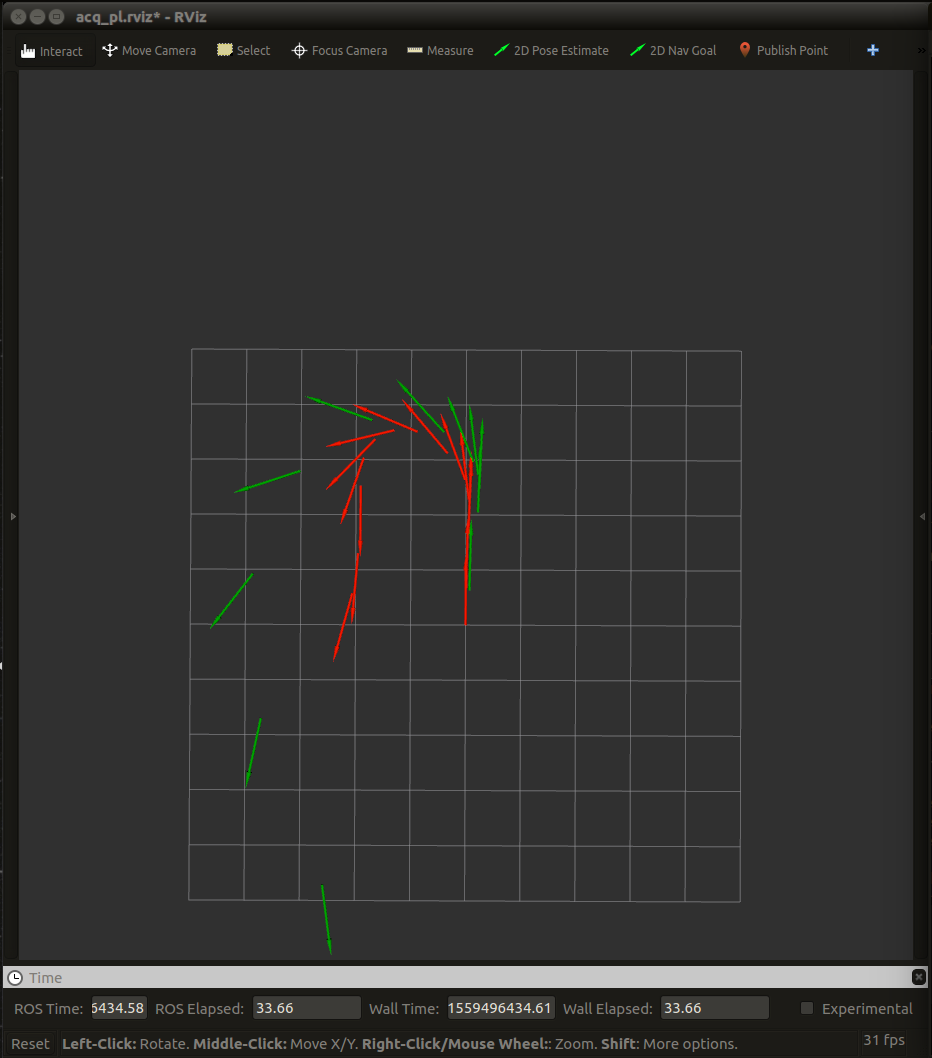
\includegraphics[scale=0.25]{rviz_sample}
	\captionsetup{justification=centering, margin=1.5cm}
	\centering
	\caption{Data Visualization in RViz. In red we are plotting the position estimated using differential drive, while in green the one using inertial navigation.}
	\centering
\end{figure}

\chapter{Localization}

As mentioned in Chapter \ref{intro_localization}, localization is the process of determining the current robot position using the measurements up to the 
current instant.\\
In the first section we will describe the Differential Drive technique, which uses the encoder measurements; in the second section we will describe the Inertial Navigation technique, which uses the IMU measurements.

\section{Differential Drive}

Differential Drive\supercite{diff_drive} is a localization technique consisting in calculating the odometry of the robot from the instant rotation of each wheel. In the following we will assume 2 drive wheels mounted on the same axis, and we will take the center of the robot on the mid-point of the wheel axis.\\
We will call, \textit{b} the length of the basis of the robot (i.e. the length of the wheel axis) and \textit{C} the center of the robot.\\

We use the two rotary encoders to have measurements about the wheels' rotations. We sample the values of the encoders at 100 Hz. Knowing the radius of each wheel, we can then compute the distance traveled by each wheel every 10ms starting from the corresponding measured rotation.\\
In the following we will call \textit{l, r} the distance traveled by the left and by the right wheel respectively.\\

\subsection{Movement in the Local Reference Frame}

We can model each instant movement as a rotation of an angle $\alpha$ around a point \textit{O} lying on the wheel axis, at a distance \textit{R} from the center of the robot (note that \textit{R} will be the radius of the robots' rotation).\\
\begin{figure}[!ht]
	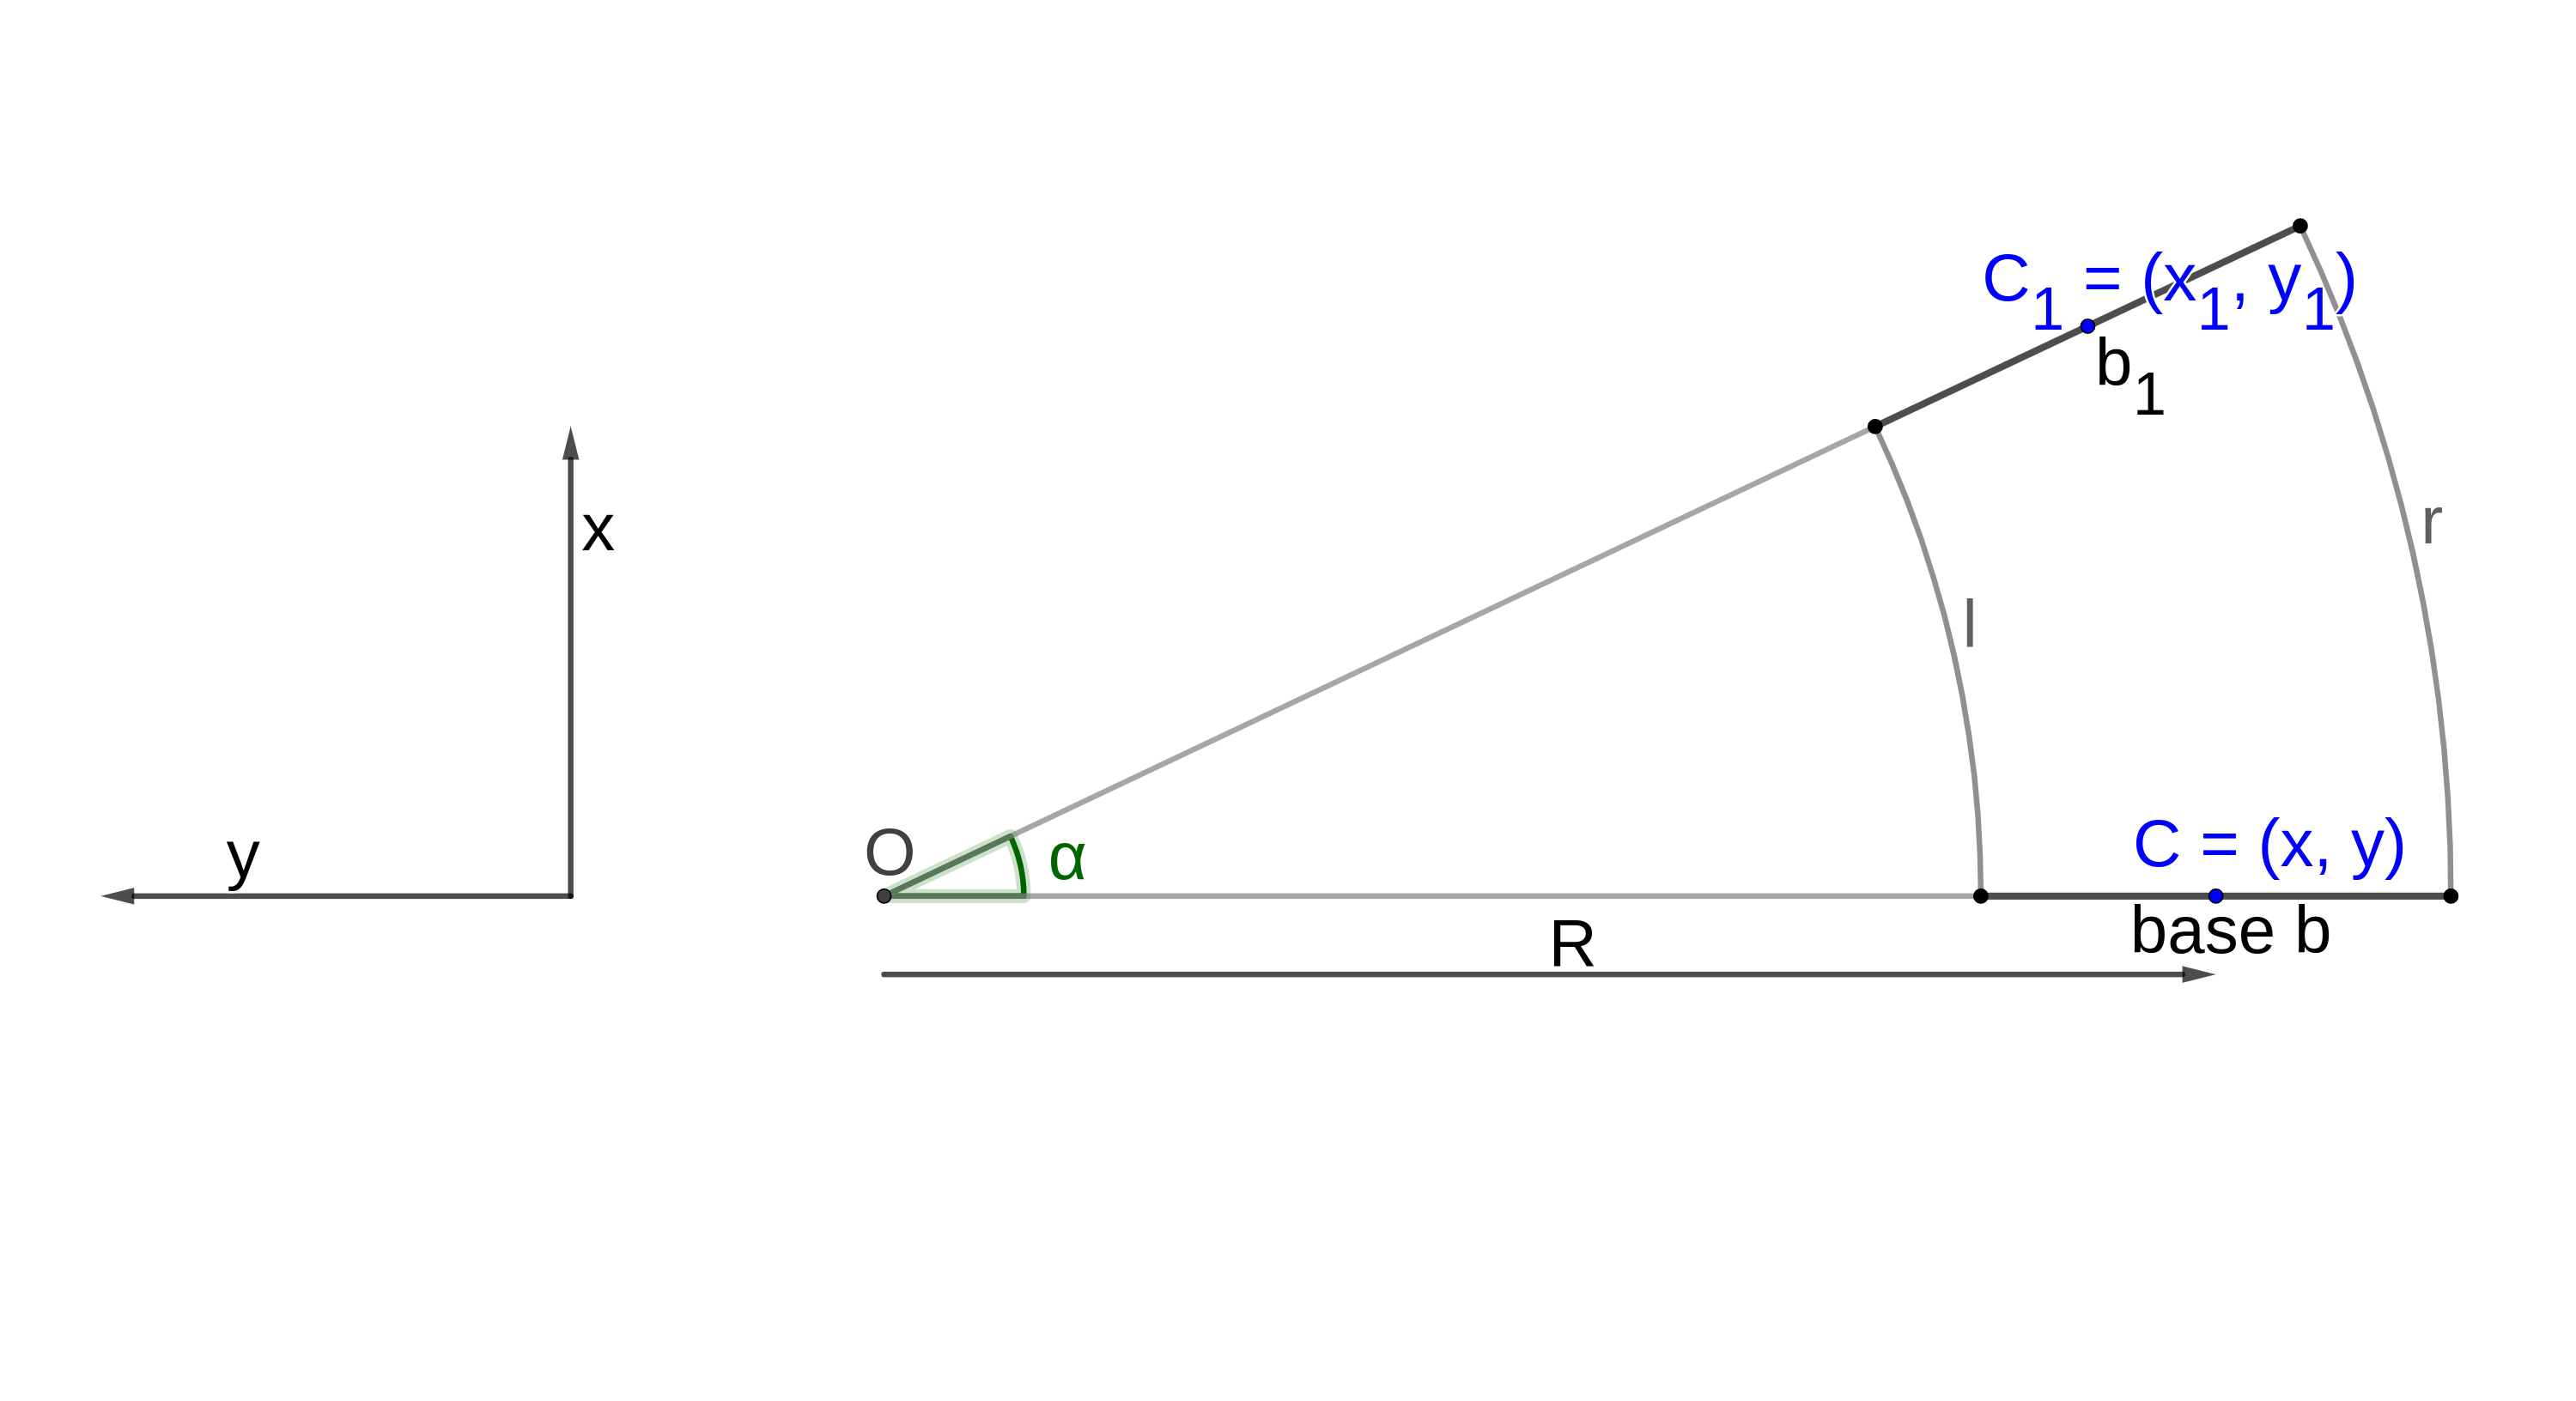
\includegraphics[scale=0.9]{differential_drive_1}
	\captionsetup{justification=centering, margin=1.5cm}
	\centering
	\caption{Model of an instantaneous movement through a rotation.}
	\centering
\end{figure}

Using this model, we can express the local movement of each wheel \textit{l, r} as a function of the parameters of the instant rotation \textit{R, }$\alpha$\footnote{The length of an arc of a circle with radius \textit{r} and subtending an angle $\alpha$ (measured in radians) with the circle center is : \textit{l} = $\alpha$ \textit{r}}.
\begin{gather*}
	r = ( R + \frac{b}{2} ) \alpha\\
	l = ( R - \frac{b}{2} ) \alpha
\end{gather*}
Respectively adding and subtracting these two equations we get:
\begin{gather*}
	r + l = 2 R \alpha\\
	r - l = b \alpha
\end{gather*}
And therefore we are able to express \textit{R, }$\alpha$ as a function of \textit{l, r}:
\begin{align}
	\alpha = \frac{r - l}{b}\\[3mm]
	R = \frac{r + l}{2 \alpha} \label{R}
\end{align}

We are now ready to express the local movement in the local reference frame:
\begin{figure}[!ht]
	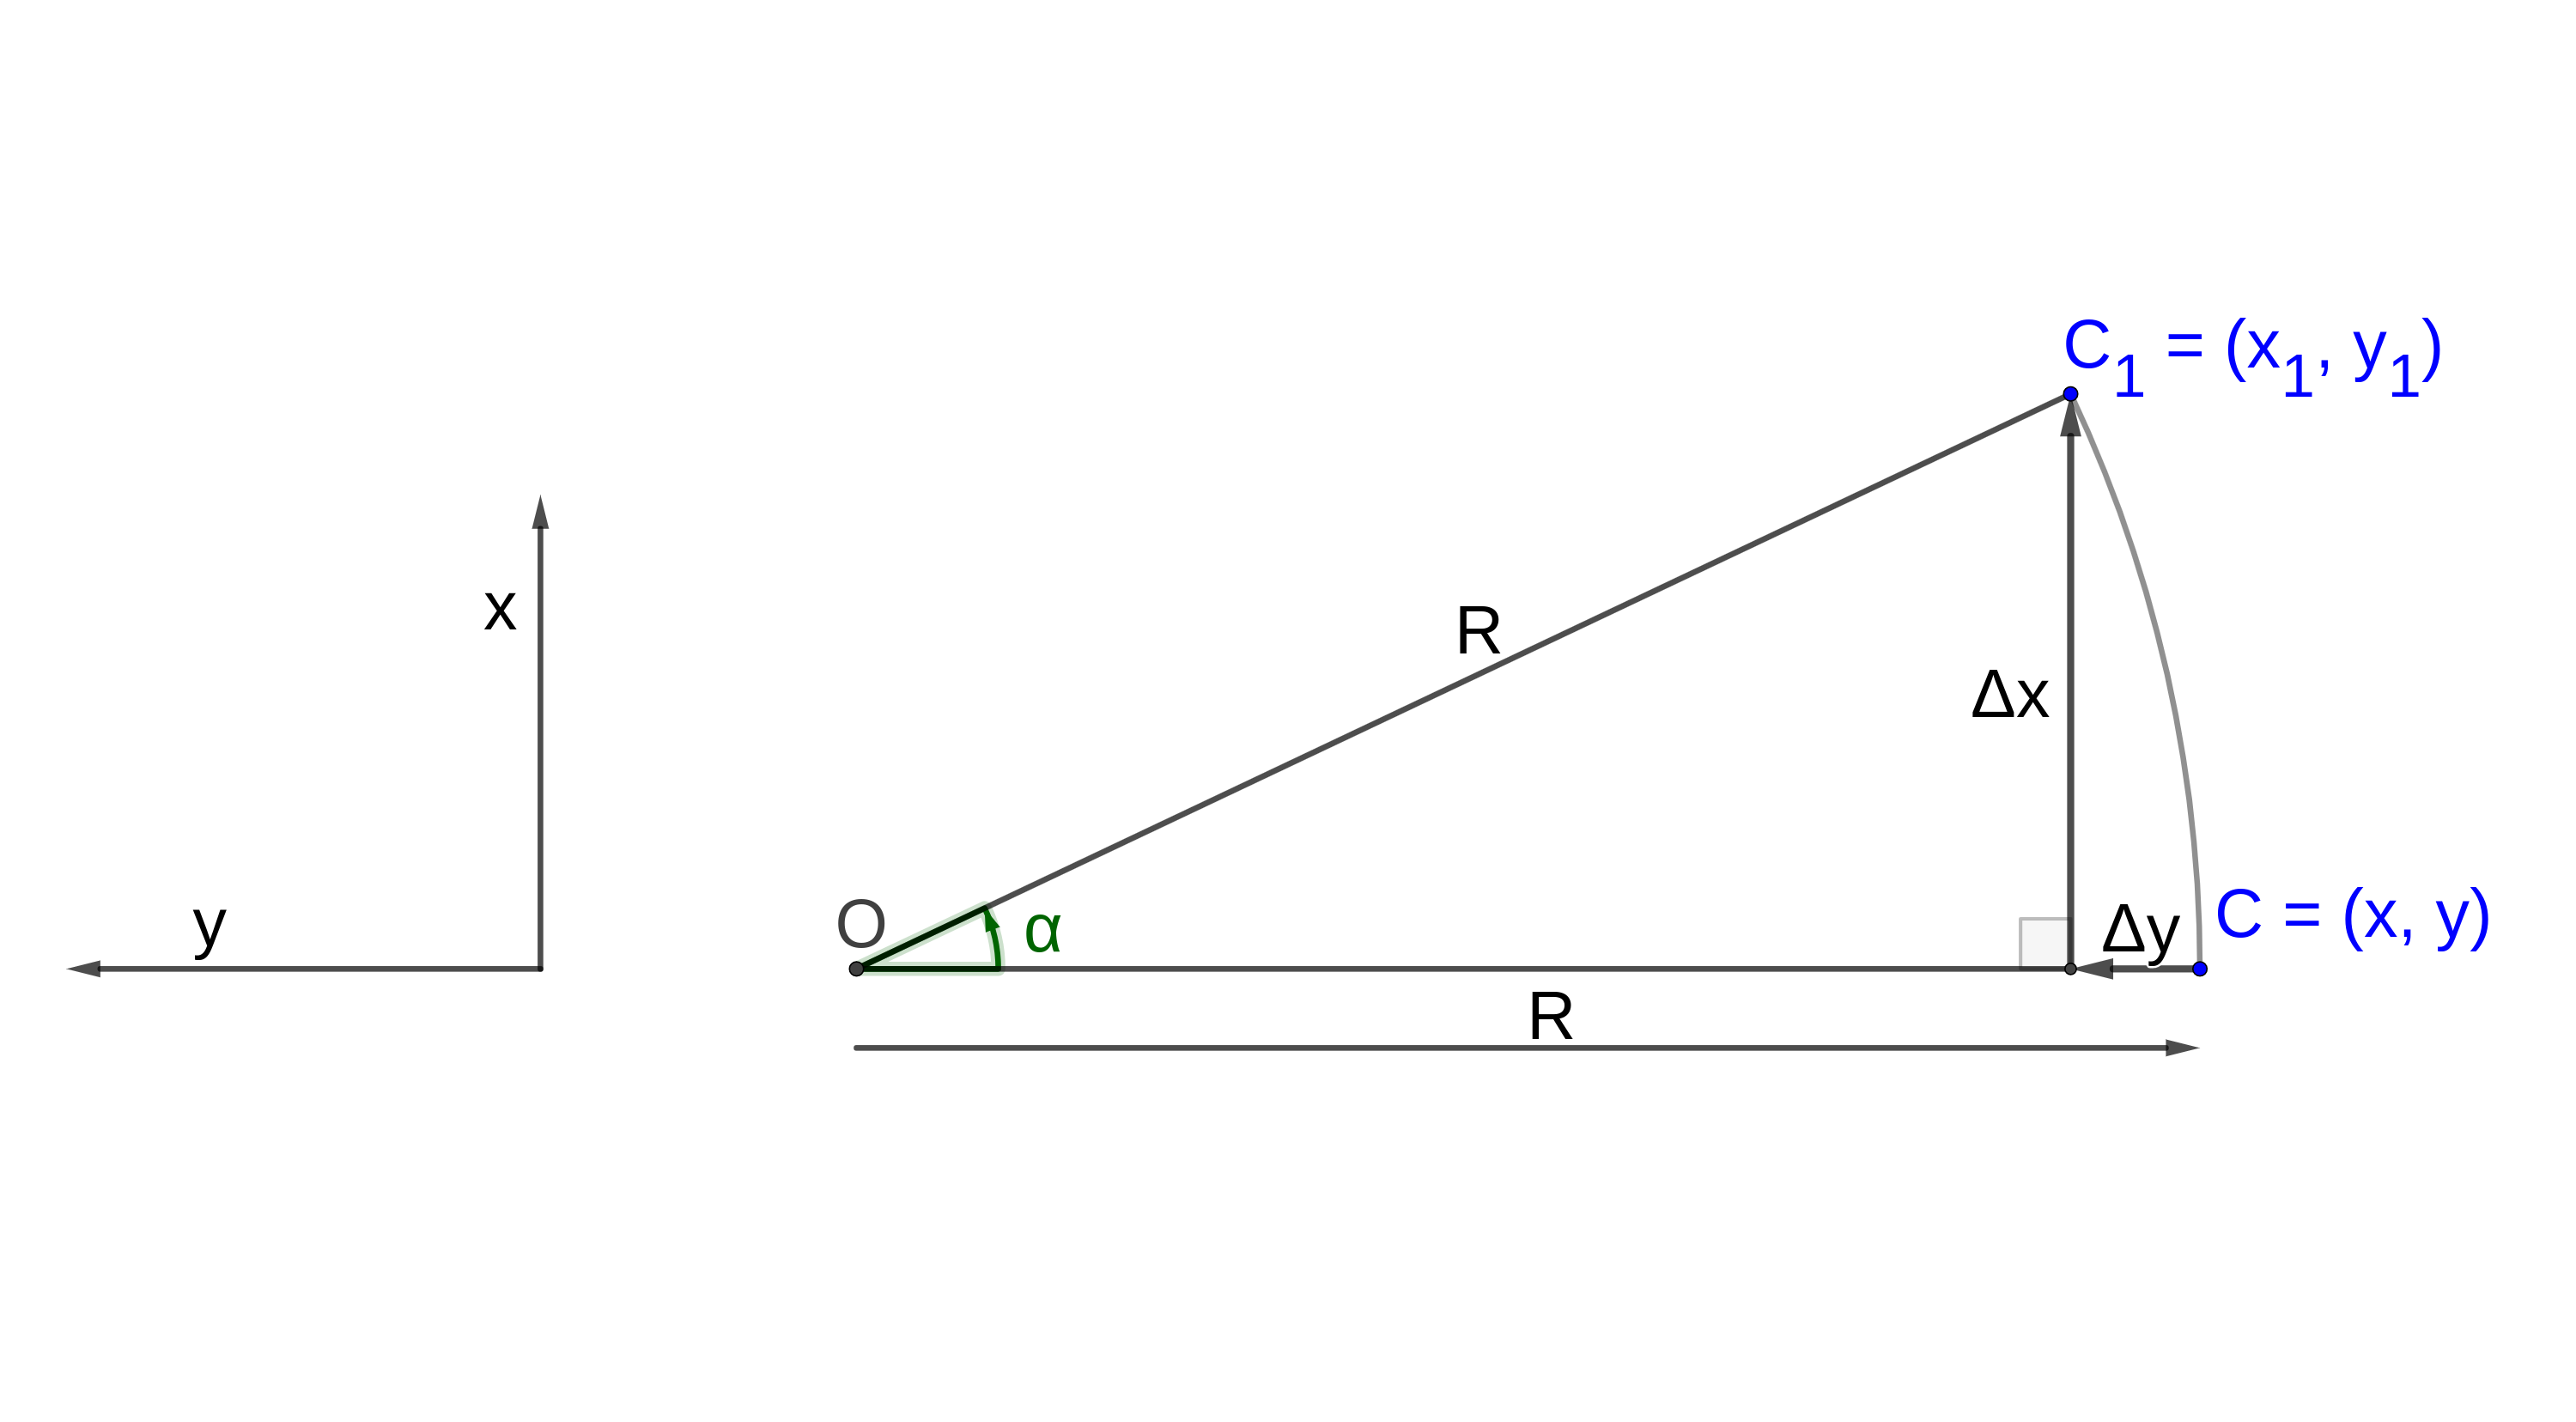
\includegraphics[scale=0.9]{differential_drive_deltas}
	\captionsetup{justification=centering, margin=1.5cm}
	\centering
	\caption{Model of an instantaneous movement through a rotation (emphasis on the local movement).}
	\centering
\end{figure}
\begin{align}
	\Delta x &= R sin \alpha\\
	\Delta y &= R - R cos \alpha = R ( 1 - cos \alpha )
\end{align}

and finally, using the \eqref{R}:

\begin{align}
	\Delta x &= \frac{r + l}{2}\text{ } \frac{sin \alpha}{\alpha}\\[3mm]
	\Delta y &= \frac{r + l}{2}\text{ } \frac{1 - cos \alpha}{\alpha}\\[3mm]
	\Delta \theta &= \alpha
\end{align}

Since $\frac{sin \alpha}{\alpha}$ and $\frac{1 - cos \alpha}{\alpha}$ have a singularity for $\alpha = 0$, we will use the corresponding Taylor-Maclaurin series\footnote{Taylor-Maclaurin series for sine and cosine:\\[1mm] $sin \alpha = \alpha - \frac{1}{3!}\alpha^3 + \frac{1}{5!}\alpha^5 - \frac{1}{7!}\alpha^7 + ...$\\[2mm] $cos \alpha = 1 - \frac{1}{2}\alpha^2 + \frac{1}{4!}\alpha^4 - \frac{1}{6!}\alpha^6 + ...$}:
\begin{align}
	\frac{sin \alpha}{\alpha} &= 1 - \frac{1}{3!}\alpha^2 + \frac{1}{5!}\alpha^4 - \frac{1}{7!}\alpha^6 + ...\\[3mm]
	\frac{1 - cos \alpha}{\alpha} &= \frac{1}{2}\alpha - \frac{1}{4!}\alpha^3 + \frac{1}{6!}\alpha^5 + ...
\end{align}


\subsection{Movement in the Global Reference Frame}\label{from_local_to_global_mov}

Having calculated the local movement, we are ready to integrate the latest sensors' measurements in the robot's global odometry.
\begin{figure}[!ht]
	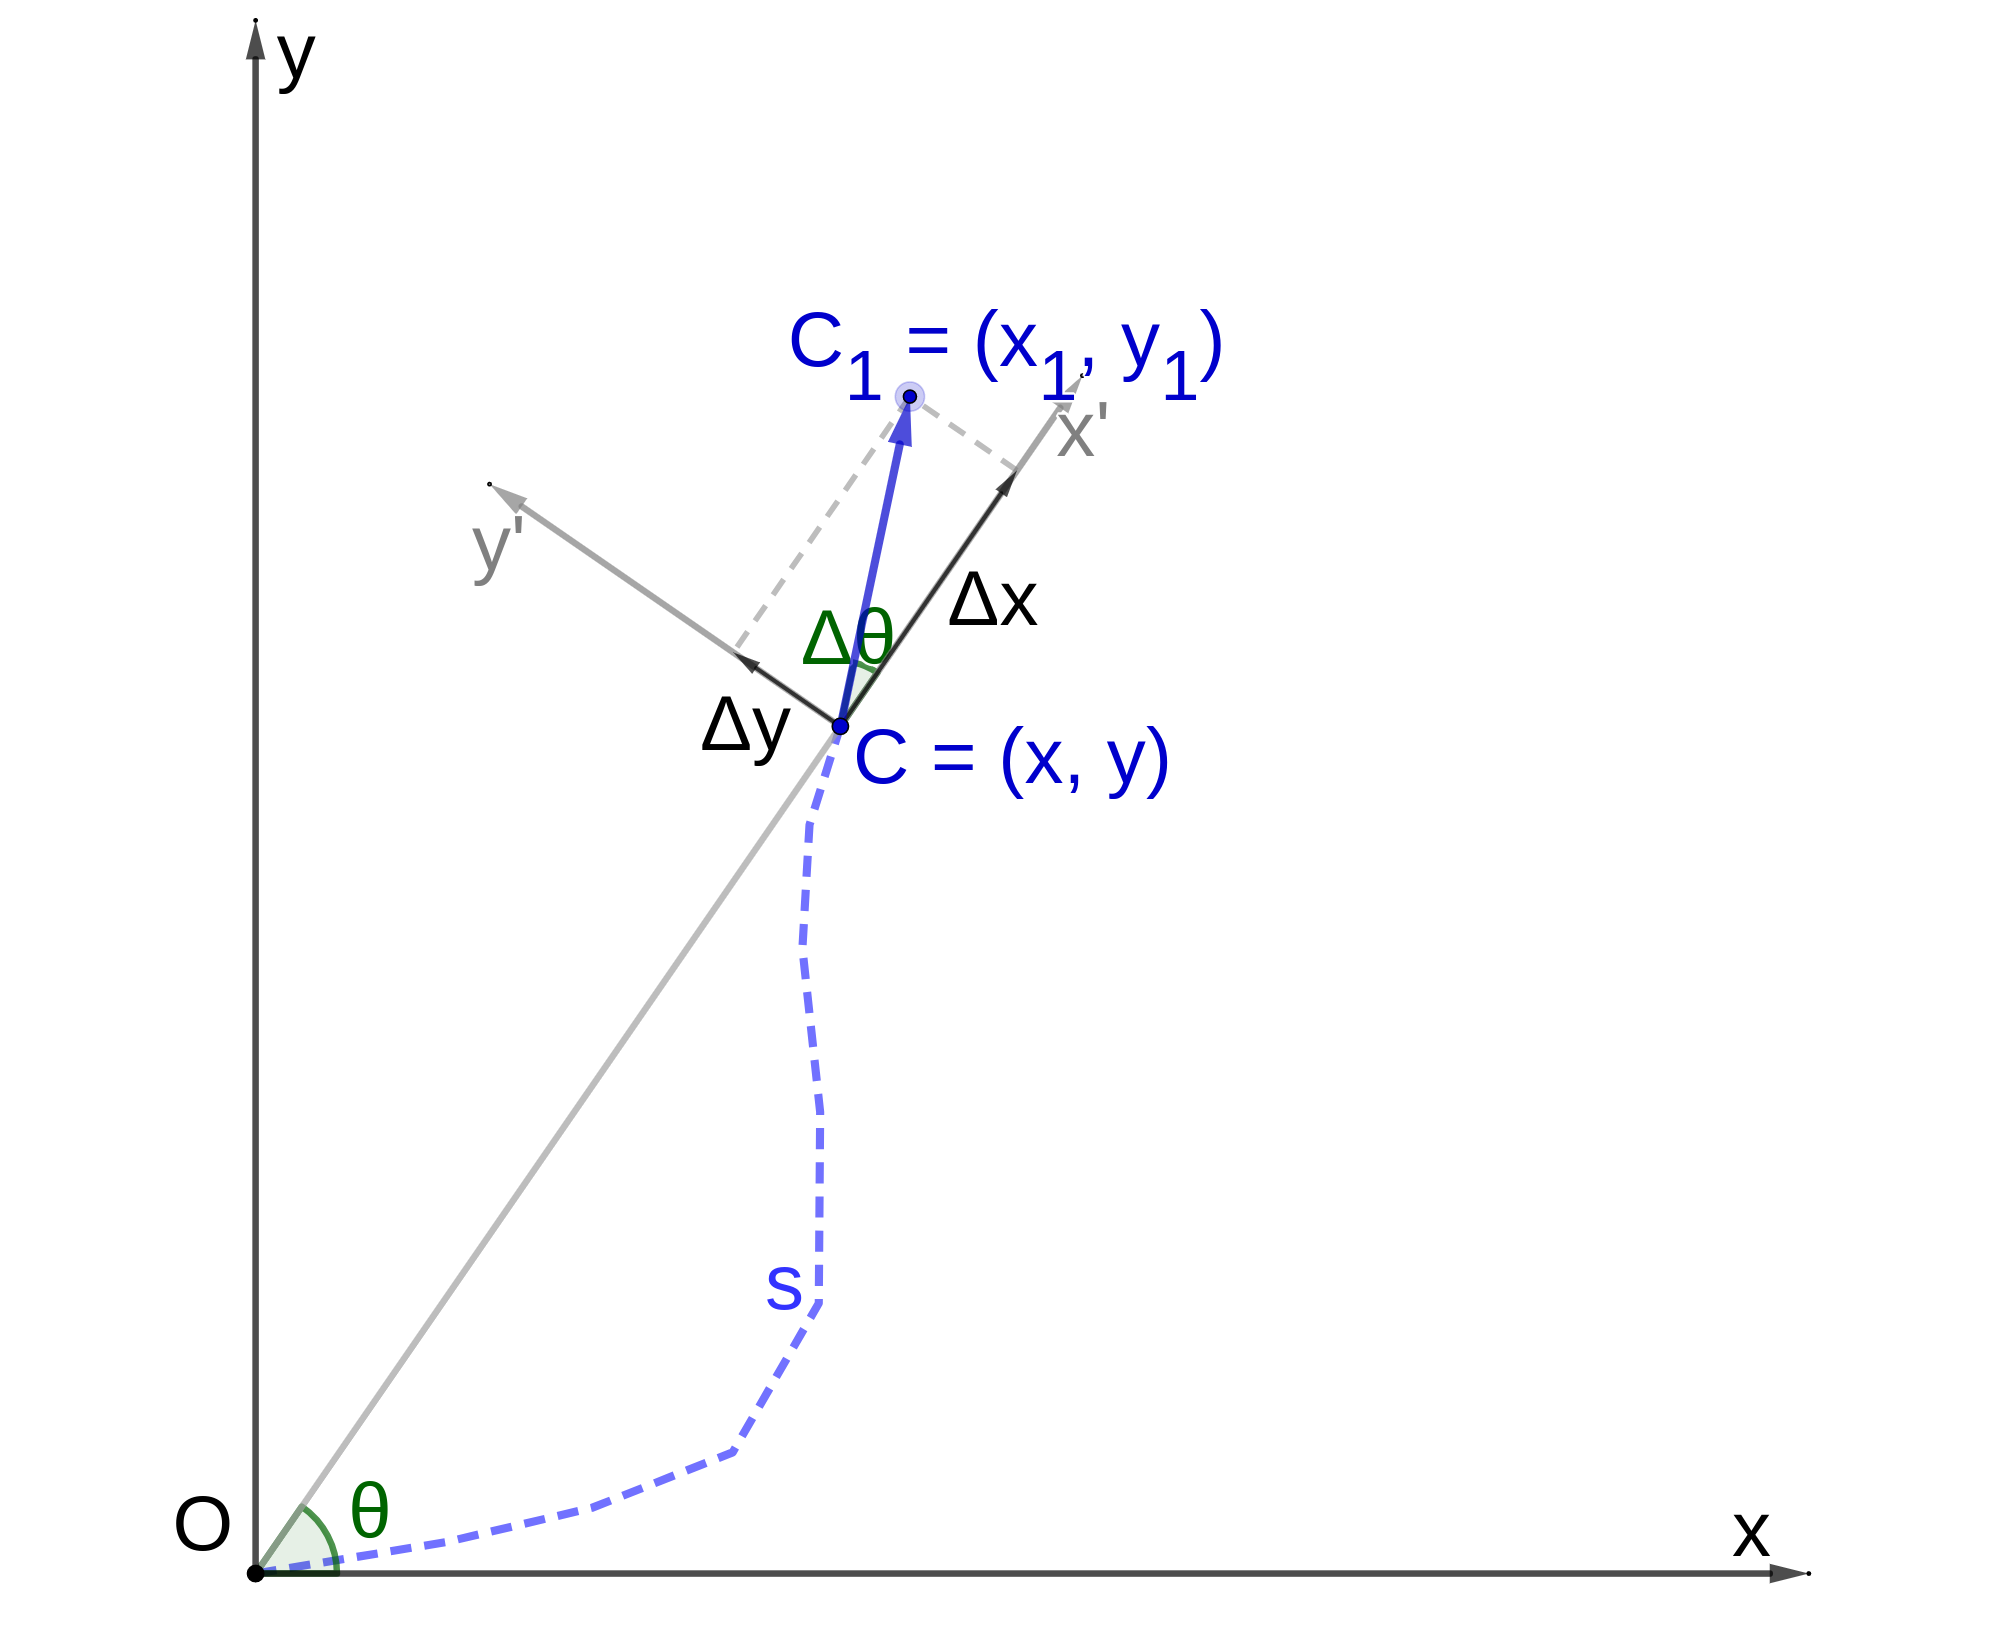
\includegraphics[scale=0.7]{differential_drive_global}
	\captionsetup{justification=centering, margin=1.5cm}
	\centering
	\caption{Movement in the Global Reference Frame.}
	\centering
\end{figure}

\begin{align}
	x &+= \Delta x cos \theta - \Delta y sin \theta\\
	y &+= \Delta x sin \theta + \Delta y cos \theta\\
	\theta &+= \Delta \theta
\end{align}

\subsection{Velocities Update}

To calculate the velocities, we will consider the movement of its central point \textit{C} as the movement fo the robot (using the \eqref{R}).
\begin{align}
	\Delta s = R \alpha = \frac{r + l}{2 \alpha} \alpha = \frac{r + l}{2}
\end{align}
At this point we can also calculate the instant robot's velocities, we will call $v_t$ the translational velocity and $v_r$ the rotational velocity:
\begin{align}
	v_t &= \frac{\Delta s}{\Delta t} = \frac{r + l}{2 \Delta t}\\[3mm]
	v_r &= \frac{\Delta \theta}{\Delta t}
\end{align}

For an implementation of Differential Drive see Appendix \ref{diff_drive_implementation}.

\section{Inertial Navigation}

Inertial navigation is a navigation technique in which the measurements provided by the accelerometer and the gyroscope are used to update the estimate of the current position and orientation of the robot with respect to a known starting point.\supercite{intro_inertial_navigation}

\subsection{Dead Reckoning}

As mentioned in Section \ref{imu_integration}, to keep track of the orientation of the robot we need to integrate the gyroscope measurements, while to keep track of the position we can integrate the accelerometer measurements obtaining the local displacement and then project it on the global axes (using the orientation determined using the gyroscope measurements).

\subsubsection{Updating Orientation}

At each sampling time interval, the gyroscope gives us the observation of the angular velocity of the robot.\\
Therefore since we observe $v_r = \der{\theta}{t}$, the integration is immediate:
\begin{align}
	\theta += v_r \Delta t
\end{align}

\subsubsection{Updating Position}

At each sampling time interval, the accelerometer provides observations on the translational accelerations along the x-axis and the y-axis of the local reference frame.\\

We will first of all calculate the instant movement in the local reference frame:
\begin{align}
	\Delta x &= v_x \Delta t + \frac{1}{2} a_x \Delta t ^ 2\\
	\Delta y &= v_y \Delta t + \frac{1}{2} a_y \Delta t ^ 2
\end{align}

At this point we can project it onto the global axes, calculating the displacement in the global reference frame (in a similar way as we did for the differential drive in Section \ref{from_local_to_global_mov}):
\begin{align}
	x &+= \Delta x cos \theta - \Delta y sin \theta\\
	y &+= \Delta x sin \theta + \Delta y cos \theta
\end{align}

\subsection{High-pass filter}

However this basic navigation algorithm is very inaccurate. One of the main reasons is that the IMU is subject to electromagnetic noise and therefore will measure non-zero accelerations and rotations even if the robot is not moving.\\
This problem is far more evident for the position rather than for the orientation, due to the double integration in the navigation algorithm which increases the error.\\

The first solution we have adopted is a simple high-pass filter, hence we ignore translational accelerations and rotational velocities below a predefined threshold ($\sim$0.4 DPS\footnote{DPS stands for Degrees Per Second} for rotational velocities and $\sim$0.05 G-Forces for translational accelerations).
\begin{figure}[!ht]
	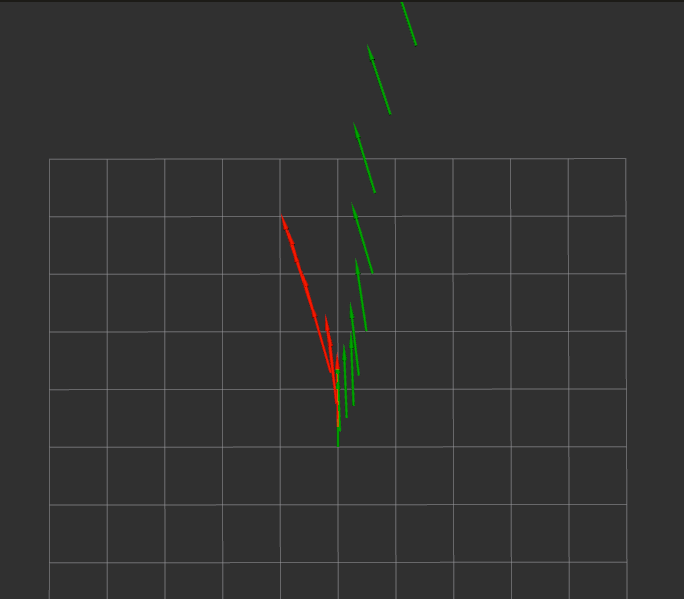
\includegraphics[scale=0.4]{encs_imu_000_trans_vel_x_y}
	\captionsetup{justification=centering, margin=1.5cm}
	\centering
	\caption{Inertial Navigation (with high-pass filter) trajectory (in green) compared to the more accurate Differential Drive trajectory (in red) visualized using Rviz.}
	\centering
\end{figure}


\subsection{Stop Motion detection}

Using the described high pass filter we have obtained a more accurate result, however once this localization algorithm has detected the movement of the robot, it is not able to detect when the robot stops. This is because even if the accelerometer no longer detects any acceleration, the previous accelerations have produced a non-zero velocity that will hardly be zeroed when the robot stops.\\

\begin{figure}[!ht]
	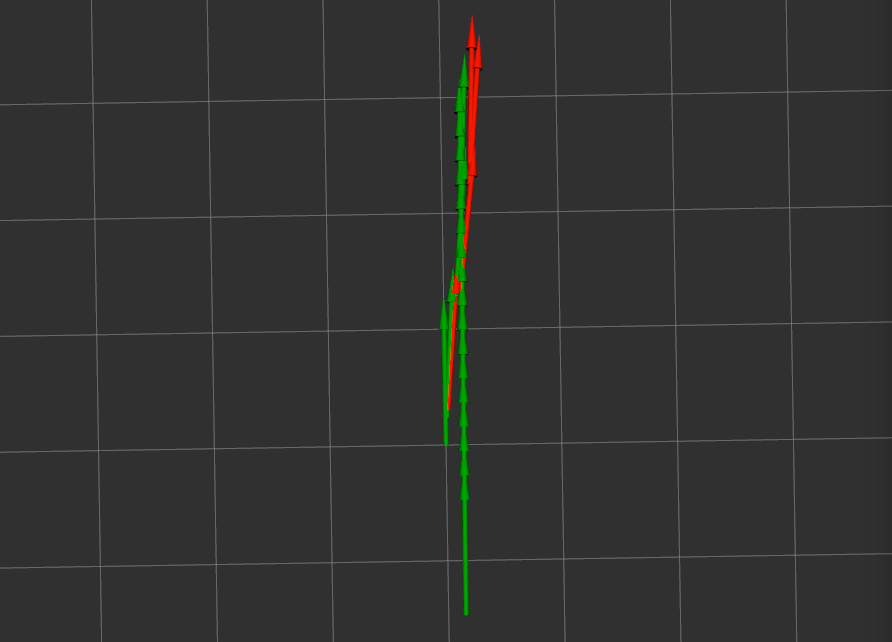
\includegraphics[scale=0.4]{encs_imu_004_imu_decel_to_neg_vel}
	\captionsetup{justification=centering, margin=1.5cm}
	\centering
	\caption{Inertial Navigation trajectory (in green) compared to the more accurate Differential Drive trajectory (in red) visualized using Rviz. We can notice how after a first phase in which the Inertial Navigation odometry followed the Differential Drive odometry, the former was unable to detect the motionless state and (having a negative velocity due to the braking phase) brought the odometry back beyond the starting position before we stopped the visualization.}
	\centering
\end{figure}

Therefore we designed a \textit{Stop Motion Detection Algorithm} which basically counts the instants with positive and negative acceleration between two motionless states and the consecutive instants with zero acceleration for each axis.\\
When the number of consecutive instants with no acceleration exceeds the difference between the instants with positive and negative acceleration scaled by a predefined factor, we assume that the robot is motionless due to friction and therefore we zero its velocity.\\
\begin{ccode}
	#define STOP_ZERO_ACCEL_OUTLIER_FILTER 5
	#define STOP_BREAKING_TRESHOLD 2

	if ( translational_acceleration_x_axis > 0. ) {
		total_time_pos_accel_x++;
		curr_time_zero_accel_x = 0;
	} else if ( translational_acceleration_x_axis < 0. ) {
		total_time_neg_accel_x++;
		curr_time_zero_accel_x = 0;
	} else //accel_x_axis == 0.
		curr_time_zero_accel_x++;	
	
	if( curr_time_zero_accel_x > STOP_ZERO_ACCEL_OUTLIER_FILTER &&
			curr_time_zero_accel_x >= abs( total_time_pos_accel_x - total_time_neg_accel_x) * STOP_BREAKING_TRESHOLD) {
		//after it has had approximately
			//the same time of positive and negative acceleration
			//we assume it is in STATIONARY state
		translational_acceleration_x_axis = 0.;
		translational_velocity_x_axis = 0.;
		
		//we reset the variables
		total_time_pos_accel_x = 0;
		total_time_neg_accel_x = 0;
	}
\end{ccode}
\captionof{lstlisting}{Implementation of the described Stop Motion Detection algorithm.}


\begin{figure}[htb]
 \centering
	\begin{subfigure}{0.3\textwidth}
		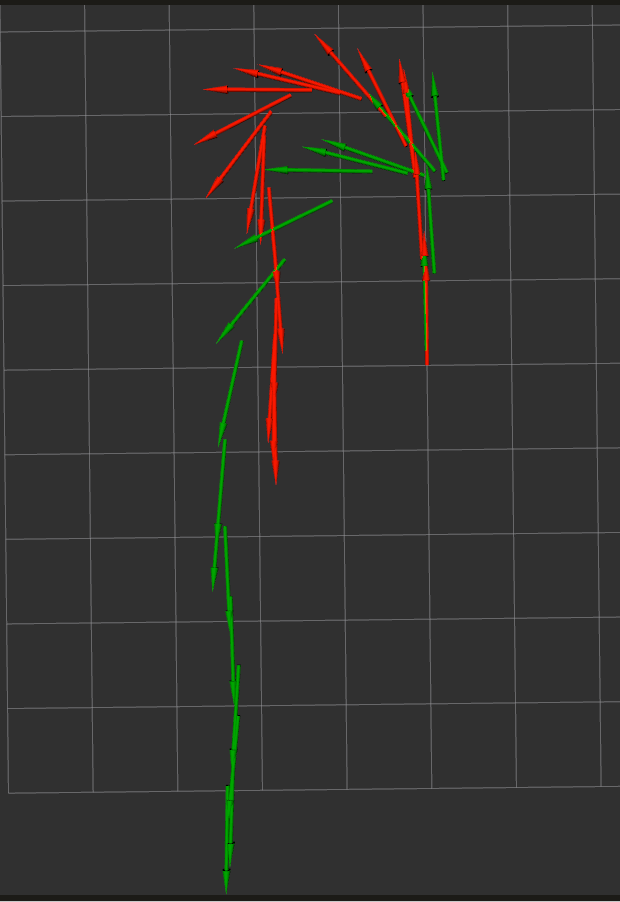
\includegraphics[width=\linewidth]{imu_encs_006_stop_motion_detecion_x_y_full}
	\end{subfigure}\hfil
	\begin{subfigure}{0.3\textwidth}
		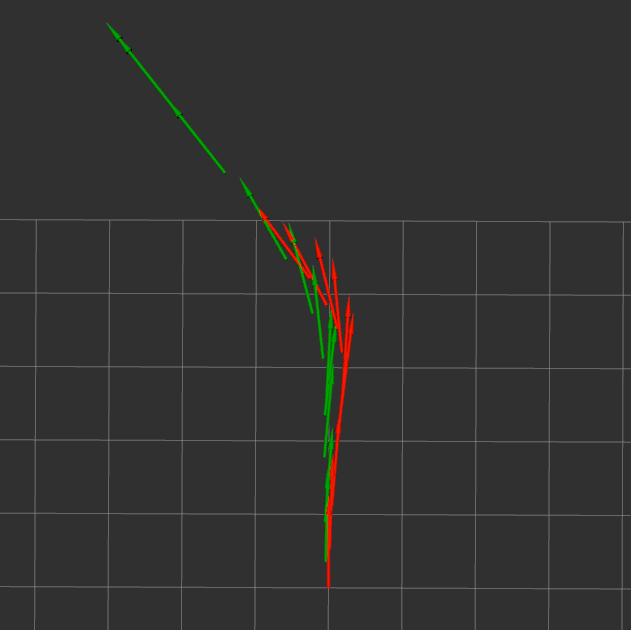
\includegraphics[width=\linewidth]{imu_encs_006_stop_motion_detection}
	\end{subfigure}\hfil
	\begin{subfigure}{0.3\textwidth}
		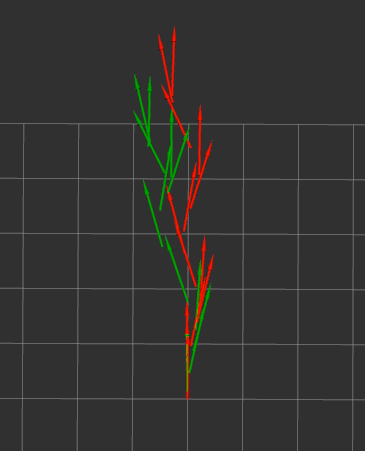
\includegraphics[width=\linewidth]{imu_encs_010_stop_motion}
	\end{subfigure}
	\captionsetup{justification=centering, margin=1.5cm}
	\caption{Inertial Navigation (with Stop Motion Detection) trajectories (in green) compared to the more accurate Differential Drive trajectories (in red) visualized using RViz.}
	\label{stop_motion_fig}
\end{figure}
In the images \ref{stop_motion_fig}, we can see how the Inertial Navigation technique, even with the high-pass filter and the Stop Motion Detection, is far less accurate than the Differential Drive technique; however it is now able to detect a motionless state, eventually with some latency, without moving the odometry to infinity.

For an implementation of Inertial Navigation see Appendix \ref{inert_nav_implementation}.

\chapter{Conclusions}

In this report we have presented the Kalman filter we used for our robot. Now we will report an evaluation test on the accuracy af the filter with respect to the odometries calculated using sensors individually.\\

We drove the robot along the following trajectory starting and ending at point A and passing through the other points in the order B, C, D, E ,F.
\begin{figure}[!ht]
	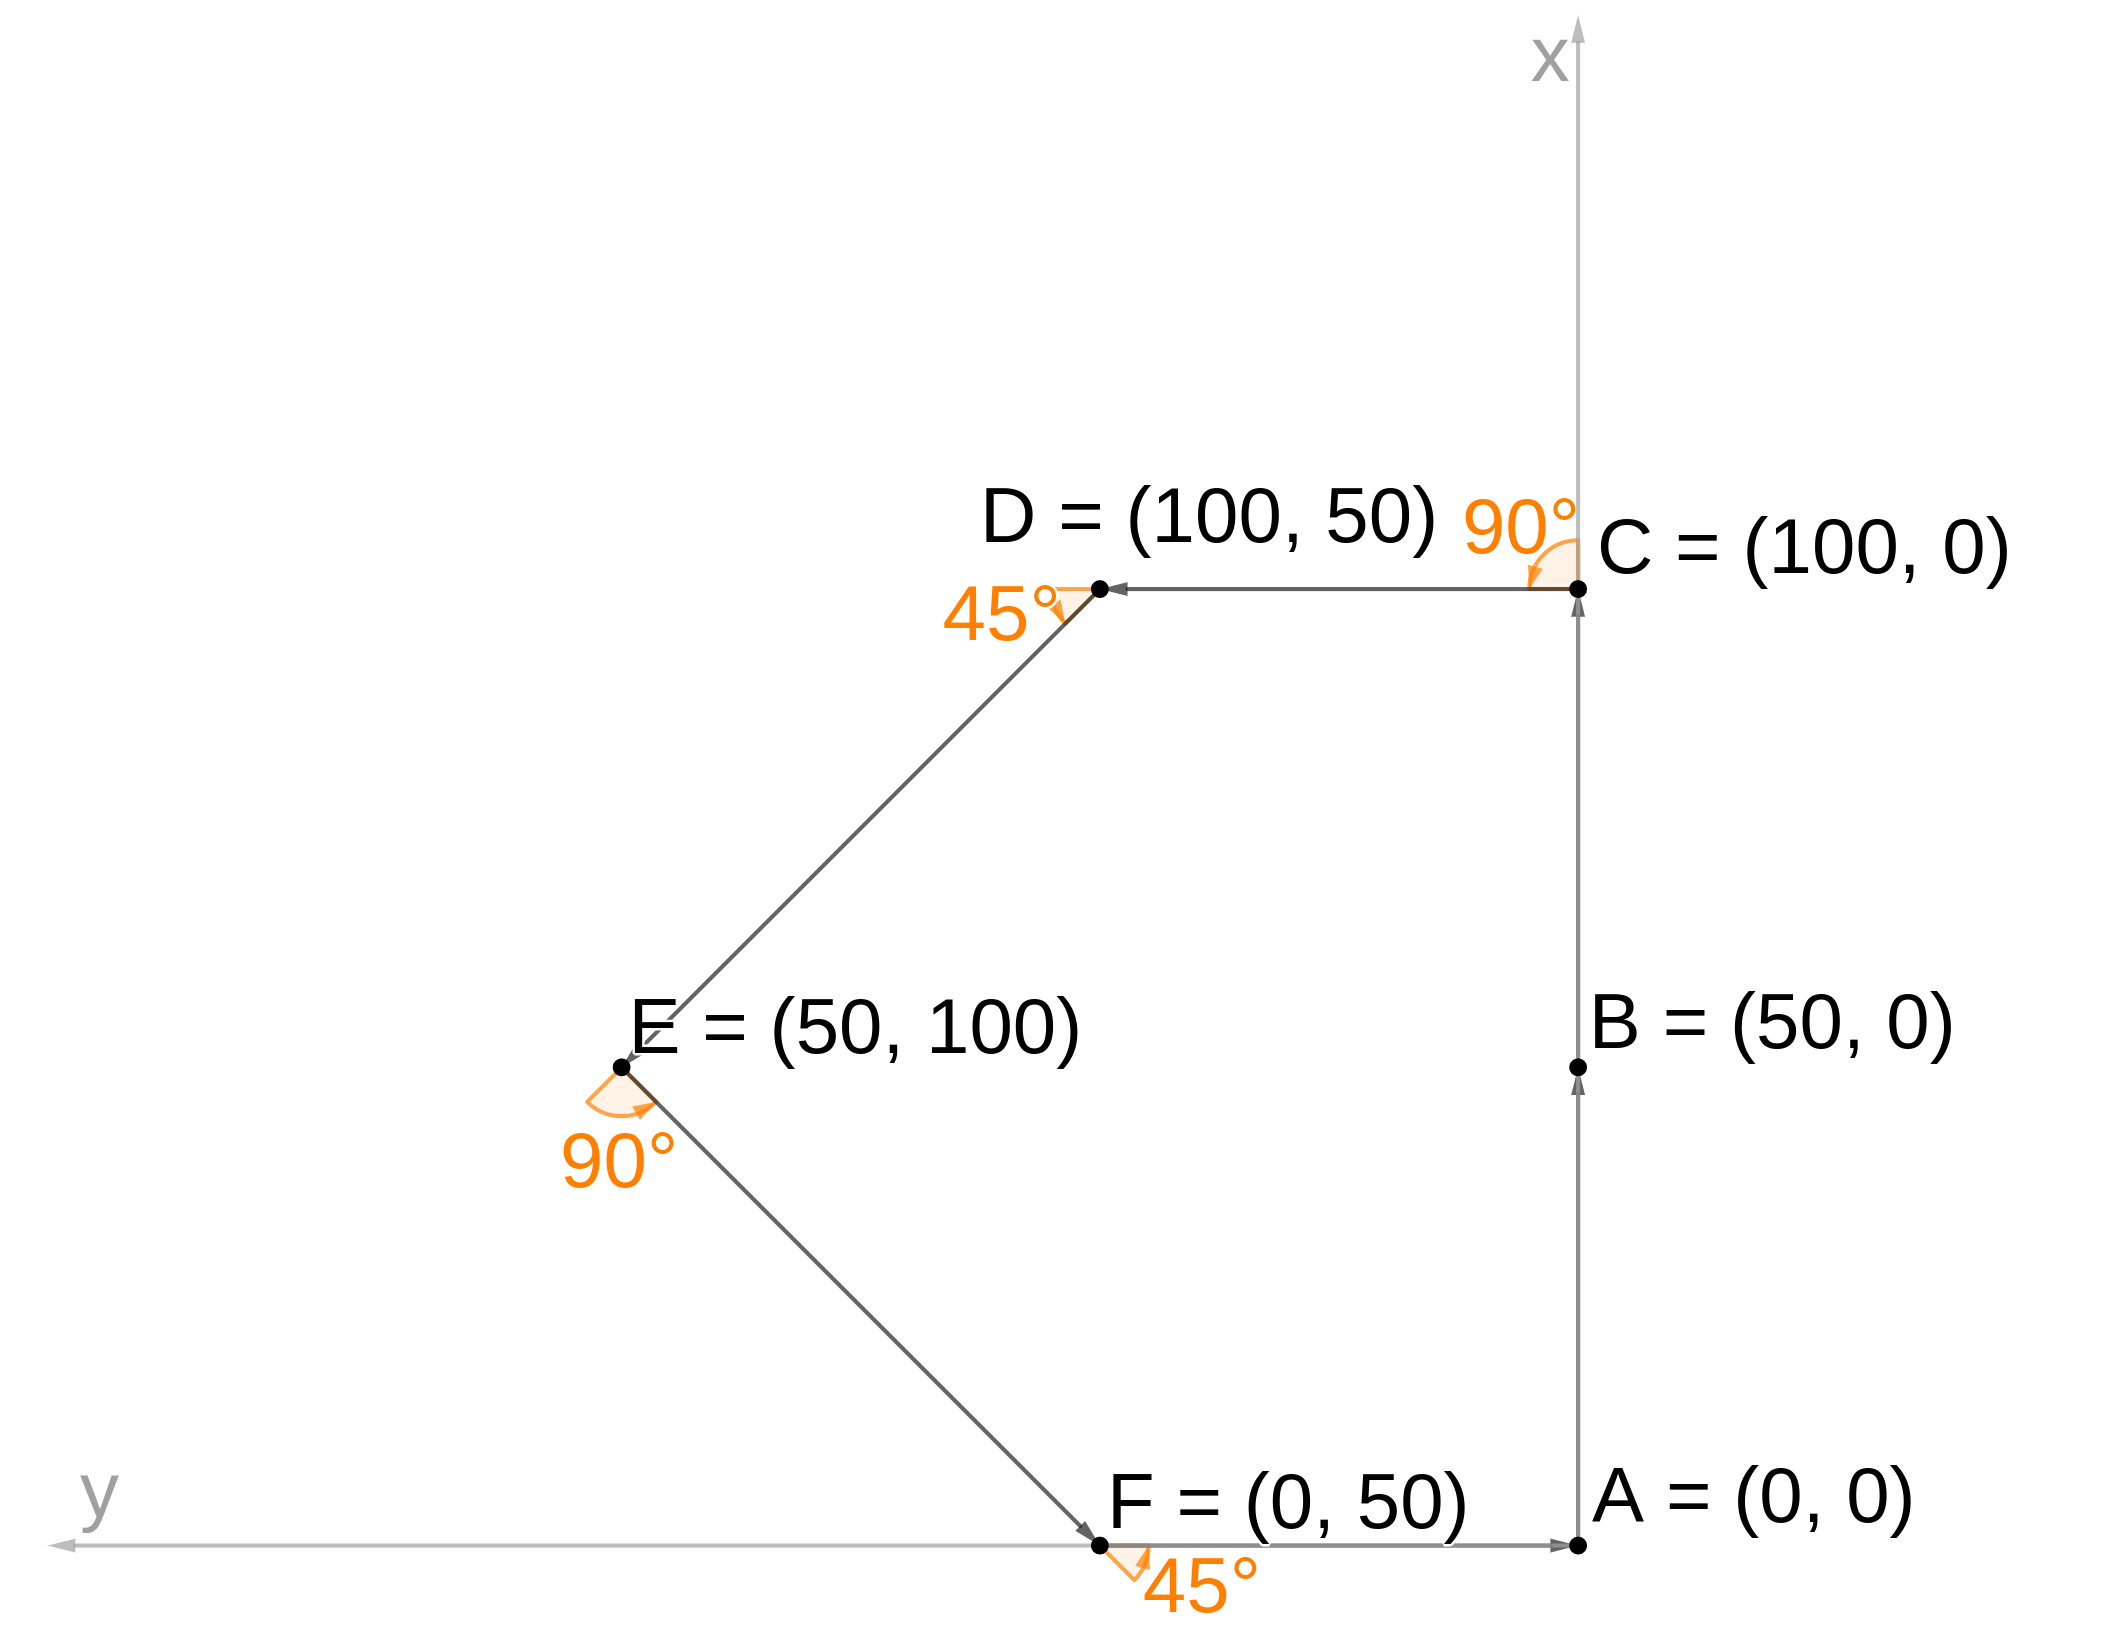
\includegraphics[scale=0.06]{test_path}
	\captionsetup{justification=centering, margin=1.5cm}
	\centering
	\caption{Expected trajectory for the test (distances are expressed in cm).}
	\centering
\end{figure}

\paragraph{Test 1}\mbox{}\\
\begin{figure}[!ht]
	\begin{subfigure}{0.35\textwidth}
		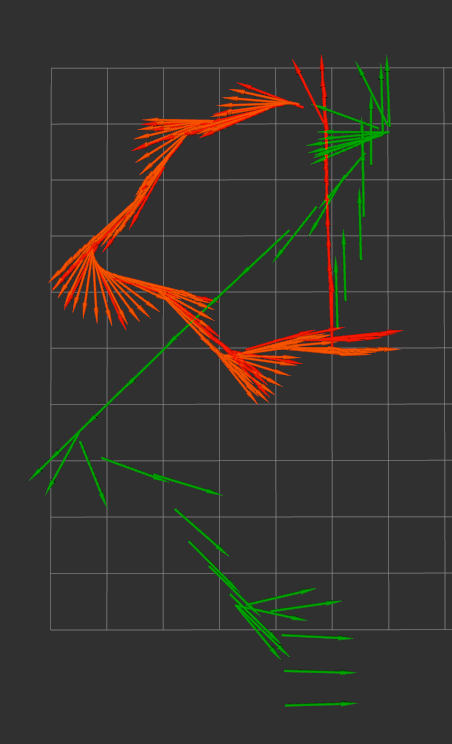
\includegraphics[width=\linewidth]{kf_test20}
	\end{subfigure}\hfil
	\begin{subfigure}{0.55\textwidth}
		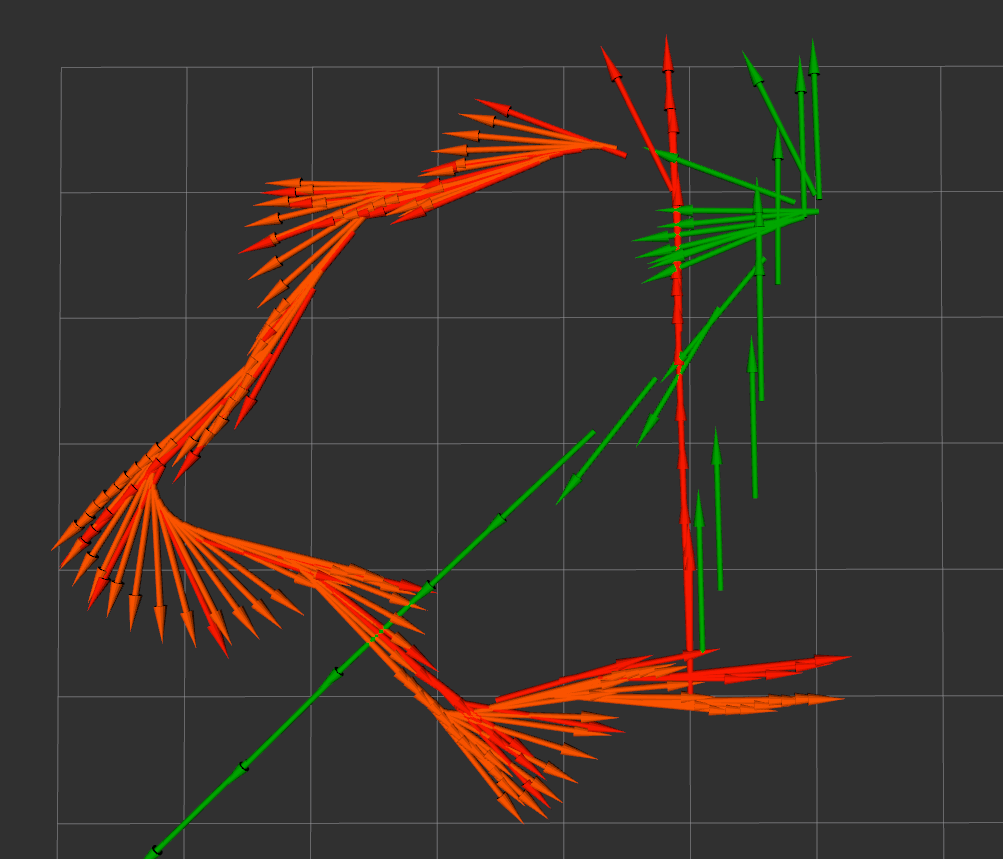
\includegraphics[width=\linewidth]{kf_test20_zoom}
	\end{subfigure}
	\captionsetup{justification=centering, margin=1.5cm}
	\centering
	\caption{Test 1 : estimated trajectories, Kalman filter trajectory in orange, Differential Drive trajectory in red, Inertial Navigation trajectory in green (visualized using RViz).}
	\centering
\end{figure}
\begin{table}[ht!]
	\centering
	\hspace*{-1cm}
	\begin{tabular}{rcccc}
		\toprule
		& \textbf{Expected} & \textbf{Kalman} & \textbf{Differential} & \textbf{Inertial}\\
		& \textbf{Position} & \textbf{Filter} & \textbf{Drive} & \textbf{Navigation}\\
		\midrule
		\textbf{A} & (0.000, 0.000, 0.000) & (0.000, 0.000, 0.000) & (0.000, 0.000, 0.000) & (0.000, 0.000, 0.000)\\
		\textbf{B} & (0.500, 0.000, 0.000) & (0.501, 0.009, 0.011) & (0.498, 0.016, 0.022) & (0.679, -0.141, 0.011)\\
		\textbf{C} & (1.000, 0.000, 0.000) & (1.002, 0.017, 0.010) & (0.999, 0.029, 0.011) & (0.991, -0.252, 0.010)\\
		\textbf{D} & (1.000, 0.500, 1.571) & (1.012, 0.523, 1.552) & (1.001, 0.534, 1.566) & (0.960, -0.256, 1.567)\\
		\textbf{E} & (0.500, 1.000, 2.356) & (0.509, 1.031, 2.325) & (0.481, 1.026, 2.349) & (-0.364, 1.117, 2.344)\\
		\textbf{F} & (0.000, 0.500, 3.927) & (-0.012, 0.518, 3.840) & (0.001, 0.479, 3.915) & (-1.136, 0.433, 3.866)\\
		\textbf{A} & (0.000, 0.000, 4.712) & (-0.009, 0.017, 4.721) & (0.046, -0.020, 4.807) & (-1.923, 0.205, 4.762)\\
		\bottomrule
	\end{tabular}
	\hspace*{-1cm}
	\caption{Test 1 : values for all the localization techniques [expressed as (x, y, theta)].}
\end{table}

By way of example we also report the final state\footnote{The state is expressed in the form $\begin{pmatrix}x & \dot{x} & \ddot{x} & y & \dot{y} & \ddot{y} & \theta & \dot{\theta}\\\end{pmatrix}\nonumber\\$} and covariance, calculated by the Kalman filter, at the end of the path after 60 seconds of motionless.
\begin{adjustwidth}{-0.6cm}{10pt}
	\begin{align}
		x &= \begin{pmatrix}
				-8.78e^{-3} & -1.14e^{-2} & -1.33e^{-2} & 1.67e^{-2} & 1.05e^{-2} & 1.24e^{-2} & 4.71 & -9.31e^{-4}\\
				\end{pmatrix}\nonumber\\
		\nonumber\\
		\Sigma_x &= \begin{pmatrix}
					2.67e^{-2} & 9.80e^{-5} & -2.37e^{-6} & 0 & 0 & 0 & 0 & 0\\
					9.80e^{-5} & 2.01e^{-4} & 2.34e^{-4} & 0 & 0 & 0 & 0 & 0\\
					-2.37e^{-6} & 2.34e^{-4} & 6.42e^{-4} & 0 & 0 & 0 & 0 & 0\\
					0 & 0 & 0 & 2.67e^{-2} & 1.00e^{-4} & 1.07e^{-8} & 0 & 0\\
					0 & 0 & 0 & 1.00e^{-4} & 2.06e^{-4} & 2.41e^{-4} & 0 & 0\\
					0 & 0 & 0 & 1.08e^{-8} & 2.41e^{-4} & 6.52e^{-4} & 0 & 0\\
					0 & 0 & 0 & 0 & 0 & 0 & 2.69e^{-7} & 2.51e^{-7}\\
					0 & 0 & 0 & 0 & 0 & 0 & 2.51e^{-7} & 5.01e^{-5}\\
				\end{pmatrix}\nonumber
	\end{align}
\end{adjustwidth}

\vspace{80pt}
\paragraph{Test 2}\mbox{}\\
\begin{figure}[!ht]
	\begin{subfigure}{0.35\textwidth}
		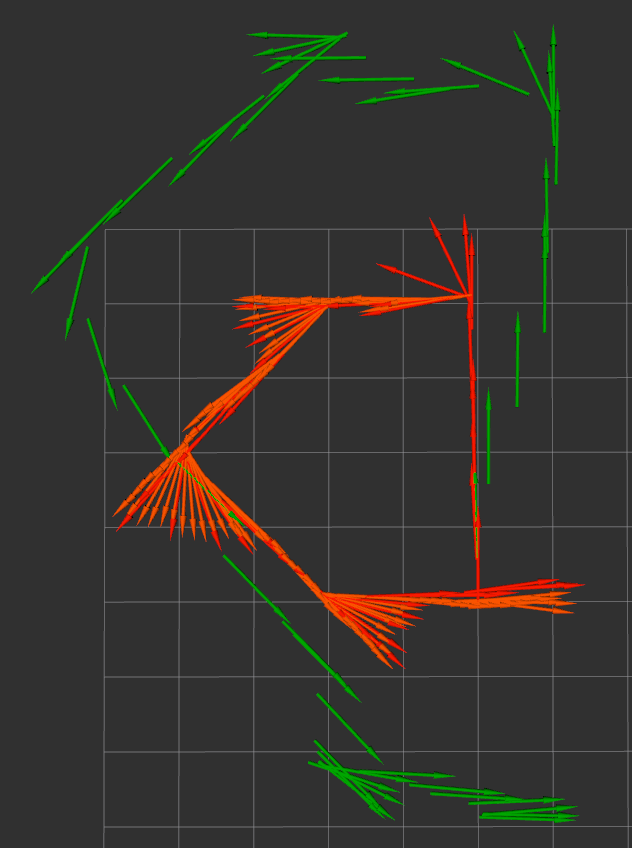
\includegraphics[width=\linewidth]{kf_test26}
	\end{subfigure}\hfil
	\begin{subfigure}{0.55\textwidth}
		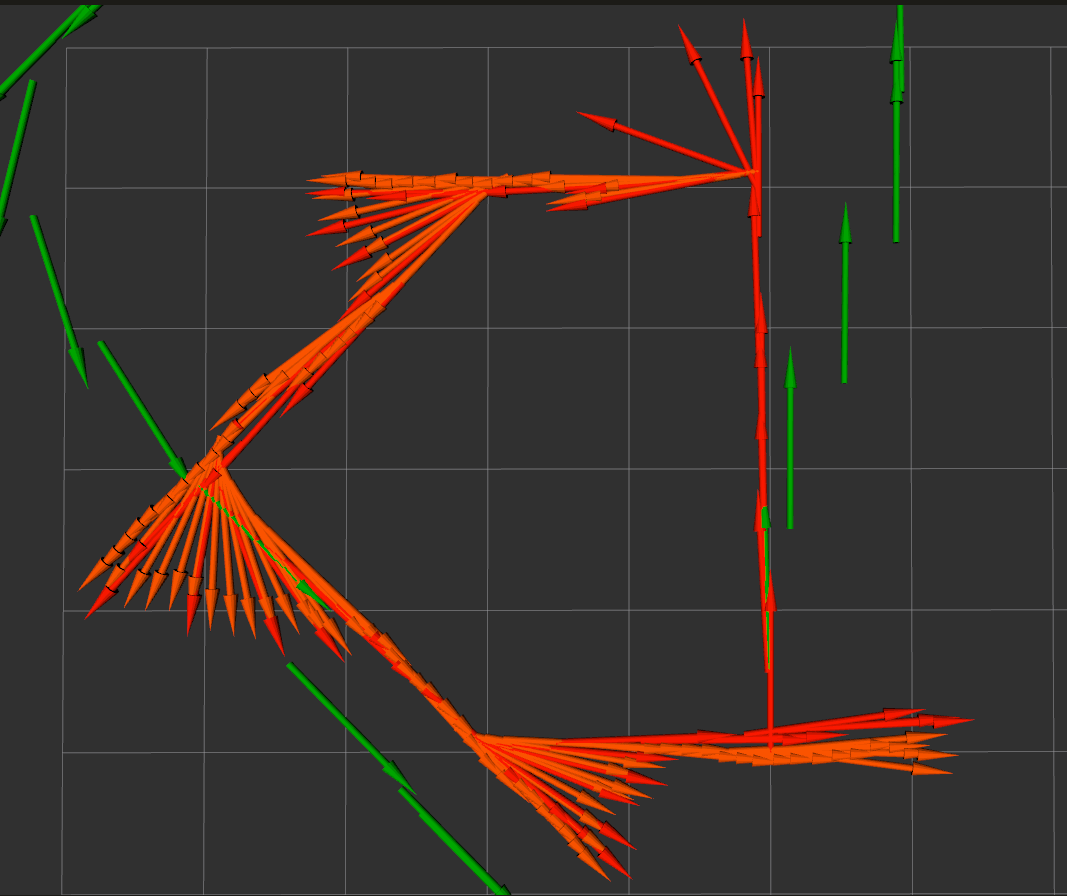
\includegraphics[width=\linewidth]{kf_test26_zoom}
	\end{subfigure}
	\captionsetup{justification=centering, margin=1.5cm}
	\centering
	\caption{Test 2 : estimated trajectories, Kalman filter trajectory in orange, Differential Drive trajectory in red, Inertial Navigation trajectory in green (visualized using RViz).}
	\centering
\end{figure}
\begin{table}[ht!]
	\centering
	\hspace*{-1.4cm}
	\begin{tabular}{rcccc}
		\toprule
		& \textbf{Expected} & \textbf{Kalman} & \textbf{Differential} & \textbf{Inertial}\\
		& \textbf{Position} & \textbf{Filter} & \textbf{Drive} & \textbf{Navigation}\\
		\midrule
		\textbf{A} & (0.000, 0.000, 0.000) & (0.000, 0.000, 0.000) & (0.000, 0.000, 0.000) & (0.000, 0.000, 0.000)\\
		\textbf{B} & (0.500, 0.000, 0.000) & (0.499, 0.000, 0.007) & (0.498, 0.012, 0.021) & (0.973, -0.224, -0.002)\\
		\textbf{C} & (1.000, 0.000, 0.000) & (1.001, 0.000, 0.006) & (0.980, 0.021, 0.076) & (1.528, -0.258, 0.056)\\
		\textbf{D} & (1.000, 0.500, 1.571) & (1.010, 0.501, 1.558) & (0.992, 0.502, 1.577) & (1.896, 0.455, 1.539)\\
		\textbf{E} & (0.500, 1.000, 2.356) & (0.516, 0.973, 2.348) & (0.524, 0.975, 2.367) & (-0.364, 1.117, 2.324)\\
		\textbf{F} & (0.000, 0.500, 3.927) & (0.006, 0.506, 3.906) & (-0.005, 0.481, 3.969) & (-0.516, 0.531, 3.911)\\
		\textbf{A} & (0.000, 0.000, 4.712) & (0.003, 0.000, 4.693) & (0.038, -0.025, 4.785) & (-0.707, -0.013, 4.691)\\
		\bottomrule
	\end{tabular}
	\hspace*{-1.4cm}
	\caption{Test 2 : values for all the localization techniques [expressed as (x, y, theta)].}
\end{table}
\newpage
By way of example we also report the final state and covariance, calculated by the Kalman filter, at the end of the path after 60 seconds of motionless.
\begin{adjustwidth}{-0.6cm}{10pt}
	\begin{align}
		x &= \begin{pmatrix}
				3.67e^{-3} & -3.57e^{-3} & -7.78e^{-3} & -2.38e^{-3} & 3.45e^{-3} & 7.69e^{-3} & 4.66 & 1.44e^{-4}\\
				\end{pmatrix}\nonumber\\
		\nonumber\\
		\Sigma_x &= \begin{pmatrix}
					1.31e^{-3} & 9.60e^{-6} & -8.84e^{-7} & 0 & 0 & 0 & 0 & 0\\
					9.60e^{-6} & 3.99e^{-5} & 8.70e^{-5} & 0 & 0 & 0 & 0 & 0\\
					-8.84e^{-7} & 8.70e^{-5} & 4.07e^{-4} & 0 & 0 & 0 & 0 & 0\\
					0 & 0 & 0 & 1.31e^{-3} & 9.60e^{6} & -8.84e^{-7} & 0 & 0\\
					0 & 0 & 0 & 9.60e^{-6} & 3.99e^{-5} & 8.70e^{-5} & 0 & 0\\
					0 & 0 & 0 & -8.84e^{-7} & 8.70e^{-5} & 6.52e^{-4} & 0 & 0\\
					0 & 0 & 0 & 0 & 0 & 0 & 1.31e^{-6} & 5.1e^{-9}\\
					0 & 0 & 0 & 0 & 0 & 0 & 5.1e^{-9} & 9.81e^{-7}\\
				\end{pmatrix}\nonumber
	\end{align}
\end{adjustwidth}
\vspace{80pt}
From these tests it emerges how the trajectory obtained with the sensor fusion (implemented through Kalman filtering) is surely far more accurate than the Inertial Navigation trajectory and it is also more accurate than the Differential Drive one. Moreover it also emerges how after a period of motionless the state is stable and the filter is very confident.\\



\begin{appendices}
	\chapter{I2C Protocol Implementation}\label{i2c_implementation}

In this appendix we present two implementations of the I2C protocol. The first one is a busy-waiting implementation, while the second one is an interrupt-driven implementation. These implementations are specific for the board used\supercite{mega2560_datasheet}, and uses the TWI module offered by the board\footnote{TWI is a variant of I2C used by manufacturers like Atmel}.

\section{I2C Control Registers}

On the board used, the TWI module is controlled by the following set of registers.
\begin{itemize}
	\item TWBR (TWI Bit Rate Register) is used to control the SCL clock frequency.
	\item TWCR (TWI Control Register) is used to control TWI operations and to poll if the current operation has ended.
	\item TWSR (TWI Status Register) is used to check the status of the TWI module and of the current transaction.
	\item TWDR (TWI Data Register) contains the data travelling on the data bus.
\end{itemize}

\section{I2C Busy-Waiting Primitives Implementation}\label{i2c_primitives}

In this section we will show a busy-waiting implementation of the primitives needed for the I2C protocol. After the start of each operation in fact the CPU polls the TWCR register until the end of the operation.
\begin{ccode}
	#define FREQ_CPU 16000000L	//cpu clock speed at 16MHz
	#define FREQ_I2C 400000L		//i2c clock speed at 400KHz


	//status indicating START condition successfully sent
	#define TWSR_START 0x08
	#define TWSR_REPEATED_START 0x10

	//status codes for Master Transmitter mode (MT)
	//status indicating address packet successfully sent
	#define TWSR_MT_SLA_ACK 0x18
	#define TWSR_MT_SLA_NACK 0x20
	//status indicating data packet successfully sent
	#define TWSR_MT_DATA_ACK 0x28
	#define TWSR_MT_DATA_NACK 0x30

	//status codes for Master Receiver mode (MR)
	//status indicating address packet successfully sent
	#define TWSR_MR_SLA_ACK 0x40
	#define TWSR_MR_SLA_NACK 0x48
	//status indicating data packet successfully sent
	#define TWSR_MR_DATA_ACK 0x50
	#define TWSR_MR_DATA_NACK 0x58

	/*
	 *	This function is used to initialize the I2c Module
	 */
	void I2C_Init(void) {
		//set te frequency of the Serial Data Clock
			//no need of prescaler, so TWSR = 0
		TWSR = 0x00;
		TWBR = ((FREQ_CPU/FREQ_I2C)-16)/2;
		
		//TWEN to enable theTWI module
		TWCR = (1<<TWEN);
	}

	static void _I2C_Start(void) {
		//TWINT to start the operation of the TWI
		//TWEN to start TWI interface
		//TWSTA to make the microcontroller master on the bus (sending a start condition)
		TWCR = (1<<TWINT)|(1<<TWEN)|(1<<TWSTA);

		//wait until current task has ended
		while (!(TWCR & (1<<TWINT)));
	}

	/*
	 *	This function is used to generate I2C Start Condition
	 *		Start Condition: SDA goes low when SCL is High
	 *	@return: 1 if ok, 0 else
	 */
	uint8_t I2C_Start(void) {
		_I2C_Start();
		
		//check if status code generated is 0x08
		return (TWSR&0xF8) == TWSR_START;
	}

	/*
	 *	This function is used to generate a repeated I2C Start Condition
	 *		Start Condition: SDA goes low when SCL is High
	 *	@return: 1 if ok, 0 else
	 */
	uint8_t I2C_Repeated_Start(void) {
		_I2C_Start();
		
		//check if status code generated is 0x10
		return (TWSR&0xF8) == TWSR_REPEATED_START;
	}

	/*
	 *	This function is used to generate I2C Stop Condition
	 *		Stop Condition: SDA goes High when SCL is High
	 */
	void I2C_Stop(void) {
		//TWSTO generates a STOP condition
		TWCR = (1<< TWINT)|(1<<TWEN)|(1<<TWSTO);
		
		 //wait for a short time
		 _delay_us(10) ;
	}

	static void _I2C_Write(unsigned char data) {
		//writes data (an 8-bit info) on TWDR
		TWDR = data;
		
		//TWINT to start the operation of the TWI
		//TWEN to start TWI interface
		TWCR = (1<< TWINT)|(1<<TWEN);
		
		//wait until current task has ended
		while (!(TWCR & (1 <<TWINT)));
	}

	/*
	 *	This function is used to send a Device Address over the bus
	 *	@param address_7bit : is the 7bit address of the slave device
	 *													you want to communicate with
	 *	@param rw : rw flag to determine if master transmitter/receiver mode
	 *								if rw = 1, read
	 *								else, write
	 *	@return: 1 if ok, 0 else
	 */
	uint8_t I2C_SendAddress(uint8_t address_7bit, uint8_t rw) {
		uint8_t addr = address_7bit<<1;
		if(rw) //read
			addr |= 1;	//set rw bit to 1
	
		_I2C_Write(addr);
		
		//checks the status code generated
		if(rw) //read, Master Receiver
			return (TWSR&0xF8) == TWSR_MR_SLA_ACK;
		 else //write, Master Transmitter
		 	return (TWSR&0xF8) == TWSR_MT_SLA_ACK;
	}

	/*
	 *	This function is used to send a byte on SDA line using I2C protocol
	 *		8bit data is sent bit-by-bit on each clock cycle
	 *			MSB(bit) is sent first and LSB(bit) is sent at last
	 *		Data is sent when SCL is low
	 *	@return: 1 if ok, 0 else
	 */
	uint8_t I2C_Write(uint8_t data) {
		_I2C_Write(data);
		
		//checks the status code generated
		return (TWSR&0xF8) == TWSR_MT_DATA_ACK;
	}

	/*
	 *	This function is used to receive a byte on SDA line using I2C protocol
	 *		8bit data is received bit-by-bit each clock and finally packed into Byte
	 *			MSB(bit) is received first and LSB(bit) is received at last
	 */
	#define ACK 1
	#define NACK 0
	uint8_t I2C_Read(uint8_t ack) {
		//TWINT to start the operation of the TWI
		//TWEN to start TWI interface
		//TWEA controls the generation of the acknowledge pulse
		//	- if 1, then ACK pulse is generated
		//	- else, not
		TWCR = (1<<TWINT)|(1<<TWEN)|(ack<<TWEA);
	
		//wait current task ended
		while (!(TWCR & (1 <<TWINT)));
	
		return TWDR;
	}
\end{ccode}

\section{I2C Busy-Waiting Implementation}

In the following section we will use the primitives defined previously, to implement the I2C protocol in busy-waiting mode.
\paragraph{Write Operations}
\begin{ccode}
	#define WRITE 0

	static void I2C_WritePreamble(uint8_t device_address, uint8_t device_reg) {
		uint8_t err;
		
		//master transmits the start condition
		err = I2C_Start();
		check_err(err, "[I2C_WritePreamble] Error transmitting the Start condition");
	
		//master transmits the (7bits) device address and the write bit (0)
		err = I2C_SendAddress(device_address, WRITE);
		check_err(err, "[I2C_WritePreamble] Error transmitting the Device Address");

		//master puts the address of the internal device register on the bus
		err = I2C_Write(device_reg);
		check_err(err, "[I2C_WritePreamble] Error transmitting the Internal Device Register");
	}

	void I2C_WriteRegister(uint8_t device_address, uint8_t device_reg, uint8_t data) {
		uint8_t err;
	
		I2C_WritePreamble(device_address, device_reg);
	
		//master puts the data to be written on the bus
		err = I2C_Write(data);
		check_err(err, "[I2C_WriteRegister] Error transmitting the data to be written");

		I2C_Stop();
	}
	
	void I2C_WriteNRegisters(uint8_t device_address, uint8_t device_reg_start, int n, uint8_t* data) {
		uint8_t err;
	
		I2C_WritePreamble(device_address, device_reg_start);
	
		//master puts the data to be written on the bus, one byte at the time
		int i;
		for(i=0; i<n; i++) {
			err = I2C_Write(data[i]);
			check_err(err, "[I2C_WriteNRegisters] Error transmitting the data to be written");
		}
		I2C_Stop();
	}
\end{ccode}
\paragraph{Read Operations}
\begin{ccode}
	#define READ 1
	#define WRITE 0

	static void I2C_ReadPreamble(uint8_t device_address, uint8_t device_reg) {
		uint8_t err;
		/* MASTER TRANSMITTER MODE */
		//master transmits the start condition
		err = I2C_Start();
		check_err(err, "[I2C_ReadPreamble] Error transmitting the Start condition");
	
		//master transmits the 7-bits device address and the write bit (0)
		err = I2C_SendAddress(device_address, WRITE);
		check_err(err, "[I2C_ReadPreamble] Error transmitting the Device Address");

		//master puts the address of the internal device register on the bus
		err = I2C_Write(device_reg);
		check_err(err, "[I2C_ReadPreamble] Error transmitting the Internal Device Register");
	
		/* MASTER RECEIVER MODE */
		//master transmits the start condition (restart)
		err = I2C_Repeated_Start();
		check_err(err, "[I2C_ReadPreamble] Error re-transmitting the Start condition");
	
		//master transmits the (7bits) device address and the read bit (1)
		err = I2C_SendAddress(device_address, READ);
		check_err(err, "[I2C_ReadPreamble] Error transmitting the Device Address");
	}

	uint8_t I2C_ReadRegister(uint8_t device_address, uint8_t device_reg) {	
		I2C_ReadPreamble(device_address, device_reg);
	
		//master reads from the bus without outputting ACK (=> NACK)
		unsigned char data = I2C_Read(0);
	
		I2C_Stop();
	
		return data;
	}

	void I2C_ReadNRegisters(uint8_t device_address, uint8_t device_reg_start, int n, uint8_t* data) {
		I2C_ReadPreamble(device_address, device_reg_start);
	
		//master reads from the bus outputting an ACK for each byte
		int i;
		for(i=0; i<n-1; i++) {
			data[i] = I2C_Read(ACK);
		}
		//master reads from the bus without outputting ACK (=> NACK)
		data[n-1] = I2C_Read(NACK);
	
		I2C_Stop();
	}
\end{ccode}

\section{I2C Interrupt-Driven Implementation}

In the following section we will present an interrupt-driven implementation of the I2C protocol. The TWI module in fact offers interrupt support, enabling the application software to carry on other operations during a TWI byte transfer.\\

When the TWINT Flag is asserted, the TWI has finished an operation and awaits application response. In this case, the TWI Status Register (TWSR) contains a value indicating the current state of the TWI bus. The application software can then decide how the TWI should behave in the next TWI bus cycle by manipulating the TWCR and TWDR Registers\supercite{mega2560_datasheet}.

\paragraph{I2C Operations Handling}
We have decided to store the operations in a global queue that the ISR of the TWI module will automatically process.\\
Each operation has a set of attributes:
\begin{itemize}
	\item the address of the slave device involved in the operation,
	\item a data buffer containing the data to be sent to the slave for write operations, or the data sent by the slave for read operations,
	\item the length of the buffer, indicating the number of bytes to write or read,
	\item the address of a post process function which will be fired at the end of the operation for any further processing to be done on the data in the buffer.\\In the implementation of the firmware, we have used the post process function in order to store the values returned by a read operation in the wanted memory locations.
\end{itemize}
\begin{ccode}
	typedef void(*PostProcessFunction_t)(uint8_t* buffer, uint8_t buflen);

	typedef struct I2C_Operation {
		struct I2C_Operation* next;	//linked list of remaining ops
		uint8_t device_address;//7 bits for device_address, 1 bit for read/write
	
		//note: if write op, device_reg will be first byte in buffer
			// if read op, buffer starts as empty
		uint8_t* buffer;	//full if write, empty if read
		uint8_t buflen;		//length of the buffer (#data to read/write)
		uint8_t bufpos;		//current pos in buffer
	
		PostProcessFunction_t post_process_fn; //to store values if it was a read op
	} I2C_Operation;
\end{ccode}

\paragraph{TWI Module Initialization}
The main difference between this and the previous (\ref{i2c_primitives}) TWI initialization is that this time we must enable the generation of interrupts by the TWI module.
\begin{ccode}
	#define FREQ_CPU 16000000L	//cpu clock spedd at 16MHz
	#define FREQ_I2C 400000L		//i2c clock spped at 400KHz


	//status indicating START condition successfully sent
	#define TWSR_START 0x08
	#define TWSR_REPEATED_START 0x10
	#define TWSR_SLARW_ARB_LOST 0x38

	//status codes for Master Transmitter mode (MT)
	#define TWSR_MT_SLA_ACK 0x18
	#define TWSR_MT_SLA_NACK 0x20
	#define TWSR_MT_DATA_ACK 0x28
	#define TWSR_MT_DATA_NACK 0x30

	//status codes for Master Receiver mode (MR)
	#define TWSR_MR_SLA_ACK 0x40
	#define TWSR_MR_SLA_NACK 0x48
	#define TWSR_MR_DATA_ACK 0x50
	#define TWSR_MR_DATA_NACK 0x58

	static volatile I2C_Operation* global_I2C_ops;

	void I2C_Init(void) {
		cli();
	
		//set te frequency of the Serial Data Clock
		TWSR = 0x00;
		TWBR = ((FREQ_CPU/FREQ_I2C)-16)/2;
	
		//Active internal pull-up resistors for SCL and SDA
			//on atmega 2560 they are PD0 and PD1
		PORTD |= 1|(1<<1);

		// Disable slave mode
		TWAR = 0;
	
		//TWEN: TWI Enable, to start TWI interface
		//TWIE : TWI Interrupt Enable in TWCR
		TWCR = (1<<TWEN)|(1<<TWIE);
		sei();
	}
\end{ccode}

\paragraph{I2C Exposed Function}
The following is the primitive exposed to the CPU to enqueue I2C operations.
\begin{ccode}
	void I2C_Enqueue_Operation(uint8_t device_address_7bit, uint8_t rw, uint8_t n, uint8_t* data, PostProcessFunction_t post_process_fn) {
		if( n <= 0 )	// no empty operations in the queue
			return;
	
		I2C_Operation* op = (I2C_Operation*)malloc(sizeof(I2C_Operation));
	
		op->next = NULL;
	
		op->device_address = (rw) ? (device_address_7bit<<1)|1 : (device_address_7bit<<1);
	
		op->buffer = (uint8_t*)malloc(n*sizeof(uint8_t));
		if( data != NULL )
			memcpy(op->buffer, data, n);
		op->buflen = n;
		op->bufpos = 0;
	
		op->post_process_fn = post_process_fn;
	
		// updates on global list of I2C_Operations will be executed atomically
		ATOMIC_BLOCK(ATOMIC_RESTORESTATE){
			if( global_I2C_ops == NULL ) {
				//if there was no pending operation,
					//appends current one
				global_I2C_ops = op;
					//and schedules it immediately
				TWCR = (1<<TWINT)|(1<<TWEN)|(1<<TWIE)|(1<<TWSTA);
			} else {
				I2C_Operation* aux = global_I2C_ops;
				while( aux->next != NULL)
					aux = aux->next;
				aux->next = op;
			}
		}
	}
\end{ccode}

\paragraph{Interrupt Service Routine}
The following ISR reads the value in the TWSR register and according to its value it decides how to proceed. The possible application software responses are based on the board's datasheet\supercite{mega2560_datasheet}.

\begin{ccode}
	ISR(TWI_vect) {
		//if there is no global I2C_Operation, exits
		if( global_I2C_ops == NULL )
			return;
	
		switch( TWSR & 0xF8 ) {	//TWI Status
			//a START (or a repeated START) condition has been transmitted
			case TWSR_START:
			case TWSR_REPEATED_START:
				//send address_7bit + read_bit
				TWDR = global_I2C_ops->device_address;
				//resets bufpos (should already be 0)
				global_I2C_ops->bufpos = 0;
				TWCR = (1<< TWINT)|(1<<TWEN)|(1<<TWIE);
				break;
		
			//arbitration lost in SLA+R/W or NACK bit
			case TWSR_SLARW_ARB_LOST:
				//start condition will be retransmitted
				TWCR = (1<<TWINT)|(1<<TWEN)|(1<<TWIE)|(1<<TWSTA);
				break;
		
		/* WRITE operation, Master Transmitter Mode */
	
			//SLA+W has been transmitted; ACK has been received
			case TWSR_MT_SLA_ACK:
				//sends first byte (device reg)
				TWDR = global_I2C_ops->buffer[global_I2C_ops->bufpos];
				global_I2C_ops->bufpos++;
				TWCR = (1<< TWINT)|(1<<TWEN)|(1<<TWIE);
				break;
		
			// SLA+W has been transmitted; NOT ACK has been received
			case TWSR_MT_SLA_NACK:
				//STOP condition followed by a START condition will be transmitted
					//and TWSTO Flag will be reset
				TWCR = (1<<TWINT)|(1<<TWEN)|(1<<TWIE)|(1<<TWSTA)|(1<<TWSTO);
				break;
		
			// data byte has been transmitted; ACK has been received
			case TWSR_MT_DATA_ACK:
				//sends next byte
				if( global_I2C_ops->bufpos < global_I2C_ops->buflen ) {
					TWDR = global_I2C_ops->buffer[global_I2C_ops->bufpos];
					global_I2C_ops->bufpos++;
					TWCR = (1<< TWINT)|(1<<TWEN)|(1<<TWIE);
					break;
				} else {
					//calls post-processing function
					if( global_I2C_ops->post_process_fn != NULL )
						(*(global_I2C_ops->post_process_fn))(global_I2C_ops->buffer, global_I2C_ops->buflen);
				
					goto next_operation;
				}
			
			case TWSR_MT_DATA_NACK:
				//STOP condition followed by a START condition will be transmitted
					//and TWSTO Flag will be reset
				TWCR = (1<<TWINT)|(1<<TWEN)|(1<<TWIE)|(1<<TWSTA)|(1<<TWSTO);
				break;

		/* READ operation, Master Receiver Mode */
		
			// SLA+R has been transmitted; ACK has been received
			case TWSR_MR_SLA_ACK:
				//if just one read, ACK pulse not generated
				if (global_I2C_ops->buflen == 1)
					TWCR = (1<<TWINT)|(1<<TWEN)|(1<<TWIE);
				else 	//else ACK is generated
					TWCR = (1<<TWINT)|(1<<TWEN)|(1<<TWIE)|(1<<TWEA);
				break;
		
			// SLA+R has been transmitted; NOT ACK has been received
			case TWSR_MR_SLA_NACK:
				//STOP condition followed by a START condition will be transmitted
					//and TWSTO Flag will be reset
				TWCR = (1<<TWINT)|(1<<TWEN)|(1<<TWIE)|(1<<TWSTA)|(1<<TWSTO);
				break;
		
			// data byte has been received; ACK has been returned
			case TWSR_MR_DATA_ACK:
				//read byte
				global_I2C_ops->buffer[global_I2C_ops->bufpos] = TWDR;
				global_I2C_ops->bufpos++;
				//if this is last operation, ACK pulse not generated
				if( global_I2C_ops->bufpos+1 == global_I2C_ops->buflen )
					TWCR = (1<<TWINT)|(1<<TWEN)|(1<<TWIE);
				else //else ACK is generated
					TWCR = (1<<TWINT)|(1<<TWEN)|(1<<TWIE)|(1<<TWEA);
				break;
		
			// data byte has been received; NOT ACK has been returned
			case TWSR_MR_DATA_NACK:
				//read byte
				global_I2C_ops->buffer[global_I2C_ops->bufpos] = TWDR;
				global_I2C_ops->bufpos++;
				//calls post-processing function
				if( global_I2C_ops->post_process_fn != NULL )
					(*(global_I2C_ops->post_process_fn))(global_I2C_ops->buffer, global_I2C_ops->buflen);
			
				goto next_operation;
					
			default:
				//it should never get here, we treated all possible Status Codes
				exit(1);
		}
		return;
	
		next_operation: {
			I2C_Operation* ended_op = global_I2C_ops;
				//forwards to next transaction
			global_I2C_ops = global_I2C_ops->next;
		
			if( global_I2C_ops != NULL )	//repeated start
				TWCR = (1<<TWINT)|(1<<TWEN)|(1<<TWIE)|(1<<TWSTA);
			else 	//if there is no next operation, transmits a stop
				TWCR = (1<<TWINT)|(1<<TWEN)|(1<<TWIE)|(1<<TWSTO);
		
			free(ended_op->buffer);
			free(ended_op);
			return;
		}
	}
\end{ccode}

	\chapter{UART Communication Implementation}\label{uart_implementation}

In this appendix we present two implementations of UART communication. The first one is a busy-waiting implementation, while the second one is an interrupt-driven implementation. These implementations are specific for the board used\supercite{mega2560_datasheet}.
\section{UART Control Registers}

On the board used, the UART serial interface is controlled by the following set of registers.
\begin{itemize}
	\item UBRRn (UART Baud Rate Register) is used to control the frequency of the byte transmission.
	\item UCSRn (UART Control and Status Register) allows to configure other aspects of the port and to poll if the UART is ready to transmit data or has received some.
	\item UDRn (UART Data Register) is the data register containing the data being sent and received.
\end{itemize}


\section{UART Busy-Waiting Implementation}\label{uart_bw}

In this first section we show an easy busy-waiting implementation of UART communication. Before starting any operation in fact the CPU polls until the end of the previous transmission.
\begin{ccode}
	//baud rate at which we want the serial to communicate
	#define UART_BAUD_RATE 38400

	//baud rate = F_CPU / (16*(UBRR+1))
	#define UBRR ( (F_CPU/16)/UART_BAUD_RATE - 1 )

	/*
	 * initializes the UART at UART_BAUD_RATE baud rate
	 */
	void UART_Init(void){
		//sets baud rate
		UBRR0H = (uint8_t)((UBRR)>>8);
		UBRR0L = (uint8_t)UBRR;
	
		//enables receiver and transmitter
		UCSR0B = (1<<RXEN0)|(1<<TXEN0);
	
		//sets data packet format: 8data, 2stop bit
		UCSR0C = (1<<UCSZ01)|(1<<UCSZ00);
	}

	/*
	 * transmits a char through the UART module.
	 *		It waits till previous char is transmitted (i.e. until UDRE is set),
	 *		then the new byte to be transmitted is loaded into UDR.
	 */
	void UART_TxByte(uint8_t data) {
		//waits until the transmit buffer is empty
		while ( !( UCSR0A & (1<<UDRE0) ) );
	
		//puts data into buffer, sends the data
		UDR0 = data;
	}

	/*
	 * receives a char from the UART module.
	 *		It waits till a char is received (i.e.till RXC is set),
	 *		then returns the received char.
	 */
	uint8_t UART_RxByte(void) {
		//waits for the data to be received
		while ( !(UCSR0A & (1<<RXC0) ) );
	
		//gets and returns received data from buffer
		return UDR0;
	}
\end{ccode}


\section{UART Interrupt-Driven Implementation}

In the following section we will present an interrupt-driven implementation of UART communication. The UART module in fact offers interrupt support, enabling the application software to carry on other operations during UART byte transfers.\\

The UART module will fire a Receive Interrupt (RX) when a new byte has been received, and a Data Register Empty Interrupt when the transmit buffer is ready to receive new data.

\paragraph{UART Data Handling}
We have decided to store the data to be transmitted and the data received in two global buffers automatically populated by the ISRs.
\begin{ccode}
	#define UART_BUFFER_SIZE 255

	typedef struct UART {
		uint8_t tx_buffer[UART_BUFFER_SIZE];
		volatile uint8_t tx_start;
		volatile uint8_t tx_end;
		volatile uint16_t tx_size;

		uint8_t rx_buffer[UART_BUFFER_SIZE];
		volatile uint8_t rx_start;
		volatile uint8_t rx_end;
		volatile uint16_t rx_size;
		
		uint16_t baudrate;
	} UART;
\end{ccode}

\paragraph{UART Module Initialization}
The main difference between this and the previous (\ref{uart_bw}) UART initialization is that this time we must enable the generation of interrupts by the UART module.
\begin{ccode}
	// Baud Rate at which we want the serial to communicate
	#define UART_BAUD_RATE 57600

	// Baud Rate = F_CPU / (16*(UBRR+1))
	#define UBRR ( (F_CPU/16)/UART_BAUD_RATE - 1 )
	
	static UART uart0;

	static void UART_buffers_init(void) {
		//initialize rx_buffer
		uart0.rx_start = 0;
		uart0.rx_end = 0;
		uart0.rx_size = 0;
	
		//initialize tx_buffer
		uart0.tx_start = 0;
		uart0.tx_end = 0;
		uart0.tx_size = 0;
	}

	/*
	 * UART_Init :
	 * 	initializes the UART at UART_BAUD_RATE baud rate
	 */
	void UART_Init(void){
		//initializes the global buffers
		UART_buffers_init();

		uart0.baudrate = UART_BAUD_RATE;
	
		//sets baud rate
		UBRR0H = (uint8_t)((UBRR)>>8);
		UBRR0L = (uint8_t)UBRR;
	
		//enables receiver and transmitter
			// RXCIE0 : RX Complete Interrupt Enable. Set to allow receive complete interrupts.
		UCSR0B = (1<<RXEN0)|(1<<TXEN0)|(1<<RXCIE0);
		//sets frame format: 8data, 2stop bit
		UCSR0C = (1<<UCSZ01)|(1<<UCSZ00);
	
		sei();
	}
\end{ccode}

\paragraph{UART Exposed Functions}
The followings are the exposed functions the CPU can use to enqueue data to be transmitted or get data that has been received.
\begin{ccode}
	/*
	 * UART_TxByte :
	 *  puts a byte in the transmit buffer
	 *		then as soon as possible it will be transmitted
	 *			through the UART module
	 */
	void UART_TxByte(uint8_t data) {
		//loops until there is some space in the buffer
		while (uart0.tx_size >= UART_BUFFER_SIZE);

		ATOMIC_BLOCK(ATOMIC_RESTORESTATE){
		  uart0.tx_buffer[uart0.tx_end] = data;
		  uart0.tx_end++;
		  
		  //if we reached the end of the circular buffer,
		  	//we go back to the beginning
			if (uart0.tx_end >= UART_BUFFER_SIZE)
				uart0.tx_end = 0;
		
			uart0.tx_size++;
		}
		
		//activates buffer empty interrupt
		UCSR0B |= (1<<UDRIE0);
	}

	/*
	 * UART_RxByte :
	 *  gets a byte from the receive buffer
	 *		@return : the received byte.
	 */
	uint8_t UART_RxByte(void) {
		//loops until there is some data in the buffer
		while(uart0.rx_size == 0);
	
		uint8_t data;
		
		ATOMIC_BLOCK(ATOMIC_RESTORESTATE){
		  data = uart0.rx_buffer[uart0.rx_start];
			uart0.rx_start++;
		
		  //if we reached the end of the circular buffer,
		  	//we go back to the beginning
			if (uart0.rx_start >= UART_BUFFER_SIZE)
				uart0.rx_start = 0;
		
			uart0.rx_size--;
		}
		
		return data;
	}
\end{ccode}

\paragraph{Interrupt Service Routines}
The first ISR is fired upon receipt of a byte, while the second one is fired when the transmit buffer is ready to transmit new data.
\begin{ccode}
	//Receive Interrupt Handler
	ISR(USART0_RX_vect) {
		//reads the new byte from UDR0,
			//and writes it in rx_buffer
	
		if (uart0.rx_size < UART_BUFFER_SIZE) {
			uart0.rx_buffer[uart0.rx_end] = UDR0;
			uart0.rx_end++;
		
		  //if we reached the end of the circular buffer,
		  	//we go back to the beginning
			if (uart0.rx_end >= UART_BUFFER_SIZE)
				uart0.rx_end = 0;
	
			uart0.rx_size++;
		}
	}

	//Data Register Empty (UDRE0) Flag
		//indicates whether the transmit buffer
		//is ready to receive new data
	ISR(USART0_UDRE_vect) {	
		//if the transmit buffer is empty
			//disables buffer empty interrupts
		if( uart0.tx_size == 0 )
			UCSR0B &= ~(1<<UDRIE0);
		else {
			//gets a byte from the tx_buff
				//adn writes it on UDR0
			UDR0 = uart0.tx_buffer[uart0.tx_start];
			uart0.tx_start++;
	
			//if we reached the end of the circular buffer,
				//we go back to the beginning
			if (uart0.tx_start >= UART_BUFFER_SIZE)
				uart0.tx_start = 0;
	
			uart0.tx_size--;
		}
	}
\end{ccode}

	\chapter{Differential Drive Implementation}\label{diff_drive_implementation}

In this appendix we present the implementation of the Differential Drive localization technique.

\begin{ccode}
	static const float sin_taylor_coeffs[] = {1., 0., -1./6., 0., 1./120., 0.};
	static const float cos_taylor_coeffs[] = {0., 1./2., 0., -1./24., 0., 1./720.};

	static void computeThetaTerms(float* sin_theta_over_theta, float* one_minus_cos_theta_over_theta, float theta) {
		*sin_theta_over_theta = 0;
		*one_minus_cos_theta_over_theta = 0;
		float theta_exp = 1;
	
		uint8_t i;
		for(i=0; i < (sizeof(sin_taylor_coeffs)/sizeof(float)); i++) {
			*sin_theta_over_theta += sin_taylor_coeffs[i]*theta_exp;
			*one_minus_cos_theta_over_theta += cos_taylor_coeffs[i]*theta_exp;
		
			theta_exp *= theta;
		}
	}

	void Encoder_OdometryUpdate(void) {
		int32_t encs_cnt[NUM_ENCODERS];
		// reads encoders' global counters in encs_cnt
	
		// calculates how many rotations where done in the last 10 ms
		int32_t left_ticks = encs_cnt[0] - encs_cnt_previous[0];
		int32_t right_ticks = encs_cnt[1] - encs_cnt_previous[1];
	
		//if encoders didn't detect any move,
			//robot didn't move
		if( left_ticks || right_ticks ) {
			//updates previous values stored
			encs_cnt_previous[0] = encs_cnt[0];
			encs_cnt_previous[1] = encs_cnt[1];
		
			//gets movement in meters
			float delta_l = left_ticks * (float)METERS_PER_ENCODER_TICK;
			float delta_r = right_ticks * (float)METERS_PER_ENCODER_TICK;
		
			float delta_plus = delta_r + delta_l;
			float delta_minus = delta_r - delta_l;
		
			float delta_theta = delta_minus / BASE_LEN;
		
			float sin_dtheta_over_dtheta, one_minus_cos_dtheta_over_dtheta;
			computeThetaTerms(&sin_dtheta_over_dtheta, &one_minus_cos_dtheta_over_dtheta, delta_theta);
		
			float delta_x = .5 * delta_plus * sin_dtheta_over_dtheta;
			float delta_y = .5 * delta_plus * one_minus_cos_dtheta_over_dtheta;		
				
			//update global odometry
				//odom_theta is the orientation angle until now
			float sin_theta = sin(odom_theta);
			float cos_theta = cos(odom_theta);
		
			odom_x += delta_x*cos_theta - delta_y*sin_theta;
			odom_y += delta_x*sin_theta + delta_y*cos_theta;
			odom_theta += delta_theta;
		
			//update global current volocities
			translational_velocity = .5 * delta_plus / delta_time;
			rotational_velocity = delta_theta / delta_time;
		}
	}
\end{ccode}

	\chapter{Inertial Navigation Implementation}\label{inert_nav_implementation}

In this appendix we present the implementation of the Inertial Navigation technique.

\begin{ccode}
	#define IMU_ANG_VEL_THRESHOLD 0.4 //DPS
	#define IMU_TRASL_ACC_THRESHOLD 0.05 //G-Forces
	#define G_FORCE_ACCEL_G 1 //g[G] = 1
	#define G_FORCE_ACCEL_M_S2 9.8 //accel[m/s^2] = accel[G-Force]*9.8

	#define STOP_BREAKING_TRESHOLD 2
	#define STOP_ZERO_ACCEL_OUTLIER_FILTER 5
	
	// HIGH-PASS FILTER for translational accelerations
		// (moreover we also convert from an acceleration in G-forces to an acceleration in m/s^2)
	translational_acceleration_x_axis = (fabs(accel_x) > IMU_TRASL_ACC_THRESHOLD) ? accel_x*G_FORCE_ACCEL_M_S2 : 0.;
	translational_acceleration_y_axis = (fabs(accel_y) > IMU_TRASL_ACC_THRESHOLD) ? accel_y*G_FORCE_ACCEL_M_S2 : 0.;
		//since we are in 2D, we'll always have a gravitational acceleration componenet on the z-axis, for which we must compensate
	translational_acceleration_z_axis = (fabs(accel_z - G_FORCE_ACCEL_G) > IMU_TRASL_ACC_THRESHOLD) ? accel_z*G_FORCE_ACCEL_M_S2 : 0.;
	
	// STOP MOTION DETECTION x axis
	if ( translational_acceleration_x_axis > 0. ) {
		total_time_pos_accel_x++;
		curr_time_zero_accel_x = 0;
	} else if ( translational_acceleration_x_axis < 0. ) {
		total_time_neg_accel_x++;
		curr_time_zero_accel_x = 0;
	} else //accel_x_axis == 0.
		curr_time_zero_accel_x++;	
	
	if( curr_time_zero_accel_x > STOP_ZERO_ACCEL_OUTLIER_FILTER && curr_time_zero_accel_x >= abs( total_time_pos_accel_x - total_time_neg_accel_x) * STOP_BREAKING_TRESHOLD) {
		//after it has had approximately
			//the same time of positive and negative acceleration
			//we assume it is in MOTIONLESS state
		translational_acceleration_x_axis = 0.;
		translational_velocity_x_axis = 0.;
		total_time_pos_accel_x = 0;
		total_time_neg_accel_x = 0;
	}
	
	// STOP MOTION DETECTION y axis
	if ( translational_acceleration_y_axis > 0. ) {
		total_time_pos_accel_y++;
		curr_time_zero_accel_y = 0;
	} else if ( translational_acceleration_y_axis < 0. ) {
		total_time_neg_accel_y++;
		curr_time_zero_accel_y = 0;
	} else //accel_x_axis == 0.
		curr_time_zero_accel_y++;	
	
	if( curr_time_zero_accel_y > STOP_ZERO_ACCEL_OUTLIER_FILTER && curr_time_zero_accel_y >= abs( total_time_pos_accel_y - total_time_neg_accel_y) * STOP_BREAKING_TRESHOLD) {
		//after it has had approximately
			//the same time of positive and negative acceleration
			//we assume it is in MOTIONLESS state
		IMU_OdometryController.odometry_status.translational_acceleration_y_axis = 0.;
		IMU_OdometryController.odometry_status.translational_velocity_y_axis = 0.;
		IMU_OdometryController.odometry_status.total_time_pos_accel_y = 0;
		IMU_OdometryController.odometry_status.total_time_neg_accel_y = 0;
	}
	
	// integrate in the local motion vector (local reference frame)
	// dx = v*t + .5*a*t*t = (v + .5*a*t)*t
	float delta_x_local = (translational_velocity_x_axis + .5*translational_acceleration_x_axis*delta_time) * delta_time;
	float delta_y_local = (translational_velocity_y_axis + .5*translational_acceleration_y_axis*delta_time) * delta_time;
		//since we are in 2D we can assume delta_z to be 0
	float delta_z_local = 0.0;//(translational_velocity_z_axis + .5*translational_acceleration_z_axis*delta_time) * delta_time;
	
	// update global odom x, y, z
	float sin_yaw = sin(imu_yaw);
	float cos_yaw = cos(imu_yaw);
	
	imu_odom_x += delta_x_local*cos_yaw - delta_y_local*sin_yaw,
	imu_odom_y += delta_x_local*sin_yaw + delta_y_local*cos_yaw;
	imu_odom_z += delta_z_local;// 0.0
	
	// integrate in translational velocities
	translational_velocity_x_axis += translational_acceleration_x_axis * delta_time;
	translational_velocity_y_axis += translational_acceleration_y_axis * delta_time;
	translational_velocity_z_axis += translational_acceleration_z_axis * delta_time;
	
	// high-pass filter for rotational velocities
	rotational_velocity_z_axis = (fabs(gyro_z) > IMU_ANG_VEL_THRESHOLD) ? gyro_z : 0.;
	rotational_velocity_y_axis = (fabs(gyro_y) > IMU_ANG_VEL_THRESHOLD) ? gyro_y : 0.;
	rotational_velocity_x_axis = (fabs(gyro_x) > IMU_ANG_VEL_THRESHOLD) ? gyro_x : 0.;
	
	// integrate in local orientation change
	float delta_yaw_deg = rotational_velocity_z_axis * delta_time;
	float delta_pitch_deg = rotational_velocity_y_axis * delta_time;
	float delta_roll_deg =	rotational_velocity_x_axis * delta_time;
	
	float delta_yaw_rad = delta_yaw_deg * M_PI / M_180;
	float delta_pitch_rad = delta_pitch_deg * M_PI / M_180;
	float delta_roll_rad = delta_roll_deg * M_PI / M_180;
	
	//update global yaw, roll, pitch
	imu_yaw += delta_yaw_rad;
 	imu_pitch += delta_pitch_rad;
 	imu_roll += delta_roll_rad;
\end{ccode}

\end{appendices}
\backmatter

\cleardoublepage

\phantomsection

%\bibliographystyle{sapthesis} % BibTeX style
\printbibliography[title=References,heading=bibintoc]

\end{document}
